%\documentclass[EJP]{ejpecp}
\documentclass[11pt]{article}
\usepackage{amsmath}
\usepackage{amssymb}
\usepackage{bbm}
%\usepackage[mathscr]{euscript}
%\usepackage{mathrsfs}
\usepackage[margin=2cm]{geometry}
\usepackage{hyperref}
\usepackage{tikz}
\usetikzlibrary{decorations.pathmorphing,arrows}
\usepackage{braket}
\usepackage{setspace}

\newtheorem{thm}{Theorem}[section]
\newtheorem{cor}[thm]{Corollary}
\newtheorem{prop}[thm]{Proposition}
\newtheorem{lem}[thm]{Lemma}
\newtheorem{lemma}[thm]{Lemma}
\newtheorem{Remark}[thm]{Remark}
\newtheorem{theorem}[thm]{Theorem}
\newtheorem{remark}[thm]{Remark}
\newtheorem{proposition}[thm]{Proposition}
\newtheorem{definition}[thm]{Definition}
\newtheorem{corollary}[thm]{Corollary}
\newtheorem{claim}[thm]{Claim}
\newtheorem{conj}[thm]{Conjecture}
\renewcommand{\thesection} {\arabic{section}}
\newenvironment{proof}{{\bf Proof:}}{\hfill$\square$\vskip.5cm}
\newenvironment{proofof}{}{\hfill$\square$\vskip.5cm}
\newcommand{\R}{\mathbb{R}}
\newcommand{\N}{\mathbb{N}}
\newcommand{\C}{\mathbb{C}}
\newcommand{\E}{\mathbf{E}}
\newcommand{\Z}{\mathbb{Z}

}
\newcommand{\D}{\mathbb{D}}
\renewcommand{\Pr}{\mathbf{P}}

\newcommand{\s}{\sigma}
\newcommand{\calF}{\mathcal{F}}
\newcommand{\sfH}{\mathsf{H}}
\newcommand{\sfi}{\mathsf{i}}
\newcommand{\sfj}{\mathsf{j}}
\newcommand{\sfn}{\mathsf{n}}
\newcommand{\sfJ}{\mathsf{J}}
\newcommand{\sfK}{\mathsf{K}}
\newcommand{\sfN}{\mathsf{N}}
\newcommand{\sfM}{\mathsf{M}}
\newcommand{\sfp}{\mathsf{p}}
\newcommand{\sfg}{\mathsf{g}}
\newcommand{\sfX}{\mathsf{X}}
\newcommand{\sfV}{\mathsf{V}}
%\newcommand{\sfZ}{\mathsf{Z}}
\newcommand{\sfw}{\mathsf{w}}
\newcommand{\sfd}{\mathsf{d}}
\newcommand{\sfD}{\mathsf{D}}
\newcommand{\Var}{\operatorname{Var}}
\renewcommand{\Re}{\operatorname{Re}}
\renewcommand{\Im}{\operatorname{Im}}
\newcommand{\x}{\boldsymbol{x}}
\newcommand{\y}{\boldsymbol{y}}
\newcommand{\br}{{\bf r}}
\newcommand{\X}{{\bf X}}
\newcommand{\Y}{{\bf Y}}
\renewcommand{\Z}{{\mathbb{Z}}}

\newcommand{\CP}{\mathbb{CP}}
\newcommand{\Hil}{\mathcal{H}}


\begin{document} 

\date{25 November 2023}

%\SUBMITTED{May 6, 2023}
%\ACCEPTED{00}
%\KEYWORDS{Random permutations}
%\AMSSUBJ{	82B05, 82B10, 60B15}

\title{Violation of Ferromagnetic Ordering of Energy Levels in Spin Rings
by Weak Paramagnetism of the Singlet}
\author{
%Mrigank${}$ \\
\large David Heson${}^{1}$, Shannon Starr${}^{2}$ and Jacob Thornton${}^{3}$\\
\textcolor{white}{.}\\
\small ${}^{1}$ Mississippi State University\\[-2pt]
\small Department of Physics and Astronomy\\[-2pt]
\small 355 Lee Boulevard\\[-2pt]
\small Mississippi State, MS 39762\\
\textcolor{white}{.}\\
\small ${}^{2}$ University of Alabama at Birmingham\\[-2pt]
\small Department of Mathematics\\[-2pt]
%\small University Hall, Room 4005\\[-2pt]
\small  1402 Tenth Avenue South\\[-2pt]
\small  Birmingham, AL 35294-1241\\[-2pt]
\small  \href{mailto:slstarr@uab.edu}{slstarr@uab.edu}\\
\textcolor{white}{.}\\
\small ${}^{3}$ Auburn University\\[-2pt]
\small Department of Chemical Engineering\\[-2pt]
\small Samford Hall\\[-2pt]
\small 182 S College Street\\[-2pt]
\small Auburn University, AL 36849
}


\maketitle


\abstract{For the quantum Heisenberg antiferromagnet with spins-$j$ on a bipartite, balanced graph, the
 Lieb-Mattis ``Ordering of energy levels'' theorem guarantees that the ground state is a spin singlet.
Moreover, defining $E^{\textrm{AF}}_{\min}(S)$ to be the minimum  eigenvalue of the Hamiltonian in the 
invariant subspace consisting of all total-spin $S$ vectors,
the Lieb-Mattis theorem guarantees the function $E^{\textrm{AF}}_{\min}(S)$
is monotonically increasing for $0\leq S\leq jN$ where $N$ is the number of vertices.
For the ferromagnet, defining $E_{\min}^{\textrm{FM}}(S)$ to be the minimum energy in the total spin-$S$ sector,
the absolute ground state is $E_{\min}^{\textrm{FM}}(jN)$.
We say that the graph satisfies ``ferromagnetic ordering of energy levels'' at order $n$, or FOEL-$n$, if  :
$\forall m$ such that $m \leq n$ and $\forall \ell$ such that $\ell \geq m$, we have
$E_{\min}^{\mathrm{FM}}(jN-m)\leq E_{\min}^{\mathrm{FM}}(jN-\ell)$.
Caputo, Liggett and Richthammer proved a theorem which generally implies  FOEL-$1$ is true.
We discuss the apparent fact that for an even length spin ring of length $L>4$,
FOEL-$n$ is violated for $n=jL-1$. The reason is that $E_{\min}^{\mathrm{FM}}(0) <E_{\min}^{\mathrm{FM}}(1)$ 
appears to be true for $L>4$.
We consider $E_{\min}^{\mathrm{FM}}(1)-E_{\min}^{\mathrm{FM}}(0)$ using the single mode approximation, to help explain this.
We supplement this with numerical computation.
Using the Bethe ansatz, Sutherland already considered the spin ring with $j=1/2$ and notably proved weak paramagnetism,
which was later also considered by Dhar and Shastry.
We review all that.}



\section{Introduction}

Consider the quantum Heisenberg ferromagnet on a length-$L$ spin ring.
The spin-$j$ Hamiltonian  is
\begin{equation}
\label{eq:HamDef}
	H_{j,L}^{\mathrm{FM}}\, =\, \sum_{\alpha=1}^{L} h_{\alpha,\alpha+1}^{(j)}\, ,\
\text{ where }\
	h_{\alpha,\alpha+1}^{(j)}\, =\, -S^{(1)}_\alpha S^{(1)}_{\alpha+1} 
	- S^{(2)}_\alpha S^{(2)}_{\alpha+1} - S^{(3)}_\alpha S^{(3)}_{\alpha+1} + j^2\, \mathbbm{1}\, .
\end{equation}
In order to implement
periodic boundary conditions on the underlying cycle graph $\mathbb{Z}/L\mathbb{Z}$ for the spin sites,
when $\alpha=L$ we interpret $S^{(\nu)}_{\alpha+1}$ to be $S^{(\nu)}_1$.

We
let $\mathbbm{1}$ denote the identity on the Hilbert space.
For $j=1/2$ the spin operators are the usual variations of the Pauli spin-$1/2$ matrices.
Namely on $\C^2$ we have the orthonormal basis $\Psi_{1/2,1/2}$ and $\Psi_{1/2,-1/2}$,
and in this basis we have the matrices for the spin operators
\begin{equation*}
	S^{(1)}\, =\, \begin{bmatrix} 0 & 1/2 \\ 1/2 & 0 \end{bmatrix}\, ,\qquad
	S^{(2)}\, =\, \begin{bmatrix} 0 & -i/2 \\ i/2 & 0 \end{bmatrix}\ \text{ and }\ 
	S^{(3)}\, =\, \begin{bmatrix} 1/2 & 0 \\ 0 & -1/2 \end{bmatrix}\, .
\end{equation*}
For $j \in \{1/2,1,3/2,2,\dots\}$, the matrices are the spin-$j$ analogue of the SU(2) spin matrices on the irreducible representation on $\C^{2j+1}$.
Namely, there is an orthonormal basis of vectors $\Psi_{j,m}$, for $m \in \{j,j-1,\dots,-j\}$ such that
$S^{(3)} \Psi_{j,m} = m \Psi_{j,m}$, and also there are raising and lowering operators $S^{+}$
and $S^{-}$ such that
\begin{equation*}
	S^{\pm} \Psi_{j,m}\, =\, \sqrt{j(j+1)-m(m\pm 1)}\, \Psi_{j,m\pm 1}\, ,
\end{equation*}
interpreting $0 \Psi_{j,j+1}$ and $0 \Psi_{j,-j-1}$ as both just the $0$ vector (since $\Psi_{j,j+1}$
and $\Psi_{j,-j-1}$ are not actual vectors in our Hilbert space, isomorphic to $\C^{2j+1}$).
For example, for $j=1/2$ we would have
\begin{equation*}
	S^{+}\, =\, \begin{bmatrix} 0 & 1 \\ 0 & 0 \end{bmatrix}\ \text{ and }\ 
	S^{-}\, =\, \begin{bmatrix} 0 & 0 \\ 1 & 0 \end{bmatrix}\, .
\end{equation*}
Then we have
\begin{equation*}
	S^{(1)}\, =\, \frac{S^+ + S^-}{2}\ \text{ and }\ S^{(2)}\, =\, \frac{S^+-S^-}{2i}\, ,\ 
\text{ so that }\ S^{\pm}\, =\, S^{(1)} \pm i S^{(2)}\, .
\end{equation*}
(By $S^{\pm}$ we mean either $S^+$ or $S^-$, with the consistent choice of the sign in each occurrence of $\pm$ in an equation, as is usual.)
If we denote for each $\alpha \in \{1,\dots,L\}$ the single site Hilbert space to be $\Hil_{\alpha}^{(j)}
\cong \C^{2j+1}$, then the total Hilbert space for all $L$ spin sites is the tensor product
\begin{equation*}
	\Hil_{[1,L]}^{(j)}\, =\, \Hil_1^{(j)} \otimes \Hil_2^{(j)} \otimes \cdots \otimes \Hil_L^{(j)}\, .
\end{equation*}
Then we also denote
\begin{equation*}
	S_x^{(\nu)}\, =\, \mathbbm{1}_{\C^{2j+1}} \otimes \cdots \otimes \mathbbm{1}_{\C^{2j+1}} 
\otimes S^{(\nu)} \otimes \mathbbm{1}_{\C^{2j+1}}  \otimes \cdots \otimes \mathbbm{1}_{\C^{2j+1}}\, ,
\end{equation*}
for $\nu \in \{1,2,3\}$,
where all factors are identities on $\C^{2j+1}$, namely $\mathbbm{1}_{\C^{2j+1}}$, except for the factor at position $x$ which is $S^{(\nu)}$.

Note that $(S^{(1)})^2+(S^{(2)})^2$ may be rewritten as $\frac{1}{2} S^+ S^- + \frac{1}{2} S^- S^+$.
So from (\ref{eq:HamDef}) we see that the Hamiltonian may be rewritten
\begin{equation*}
	H_{j,L}^{\mathrm{FM}}\, =\, \sum_{\alpha=1}^{L} \bigg(j^2\, \mathbbm{1}
-S^{(3)}_\alpha S^{(3)}_{\alpha+1}
-\frac{1}{2}\, S^{+}_\alpha S^{-}_{\alpha+1} 
-\frac{1}{2}\, S^{-}_\alpha S^{+}_{\alpha+1} \bigg)\, .
\end{equation*}
Also, the Casimir operator on $\C^{2j+1}$ (the generator of the center of the $\mathrm{SU}(2)$ representations) may be written 
\begin{equation*}
	\mathcal{C}\, =\, (S^{(1)})^2 + (S^{(2)})^2 + (S^{(3)})^2\, =\, (S^{(3)})^2 + \frac{1}{2}\, S^{+} S^{-} + \frac{1}{2}\, S^{-} S^{+}\, .
\end{equation*}
Then, since we may see for the spin raising and lowering operators on $\C^{2j+1}$ that
\begin{equation*}
	S^+ S^- \Psi_{j,m} + S^- S^+ \Psi_{j,m}\, =\, 2\big(j(j+1)-m^2) \Psi_{j,m}\, ,
\end{equation*}
for every $m=-j,-j+1,\dots,j$, we see that $\mathcal{C} \Psi_{j,m} = j(j+1) \Psi_{j,m}$.
This is consistent with the SU(2) commutation relations for the Lie bracket commutator $[A,B] = AB - BA$,
\begin{equation*}
	[S^{(1)},S^{(2)}]\, =\, i S^{(3)}\, ,\
	[S^{(2)},S^{(3)}]\, =\, i S^{(1)}\, ,\
	[S^{(3)},S^{(1)}]\, =\, i S^{(2)}\, ,\
\end{equation*}
because one sees that $\mathcal{C}$ commutes with $S^{(1)}$, $S^{(2)}$ and $S^{(3)}$.
So, as we have defined it, each $\C^{2j+1}$ is an {\em irreducible} representation of $\mathrm{SU}(2)$.
But on the tensor product Hilbert space $\Hil_{[1,L]}^{(j)}$, 
the total spin operators are
\begin{equation*}
	S^{(\nu)}_{\mathrm{tot}}\, =\, \sum_{\alpha=1}^{L} S_\alpha^{(\nu)}\, ,\  \text{ for $\nu \in \{1,2,3\}$, and }\ 
	\mathcal{C}_{\mathrm{tot}}\, =\, (S^{(1)}_{\mathrm{tot}})^2+(S^{(2)}_{\mathrm{tot}})^2+ (S^{(3)}_{\mathrm{tot}})^2\, .
\end{equation*}
Each of the total spin operators commutes with each nearest-neighbor interaction
term $h_{\alpha,\alpha+1}^{(j)}$.
So the whole Hamiltonian commutes with $S^{(1,2,3)}_{\mathrm{tot}}$.
Similarly, $H^{\mathrm{FM}}_{j,L}$ commutes with the Casimir operator
 $\mathcal{C}_{\mathrm{tot}}$.
So we may define, for each choice of half integer 
\begin{equation*}
S \in \{0,1/2,1,3/2,2,\dots\} \cap \{jL,jL-1,jL-2,\dots\}\, ,
\end{equation*}
the Hilbert subspace $\Hil^{(j)}_{[1,L]}(S)$ defined as 
\begin{equation*}
	\Hil^{(j)}_{[1,L]}(S)\, =\, \big\{\psi \in \Hil^{(j)}_{[1,L]}\, :\, \mathcal{C}_{\mathrm{tot}} \psi = S(S+1) \psi\big\}\, .
\end{equation*}
With this defined, we define the energy eigenvalue $E_{\min}^{\mathrm{FM}}(S;j,L)$ to be
\begin{equation}
\label{eq:EminDef}
	E_{\min}^{\mathrm{FM}}(S;j,L)\, =\, \min\left(\left\{\frac{\langle \psi\, ,\ H_{j,L}^{\mathrm{FM}} \psi \rangle}{\|\psi\|^2}\, :\, 
	\psi \in \Hil_{[1,L]}^{(j)}(S)\, ,\ \|\psi\|\neq 0\right\}\right)\, .
\end{equation}
By the Rayleigh-Ritz variational formula, that is the smallest eigenvalue of $H^{\mathrm{FM}}_{j,L}$
when restricted to the invariant subspace $\Hil^{(j)}_{[1,L]}(S)$.
When there is no confusion, we may write $E_{\min}^{\mathrm{FM}}(S)$ in place of  $E_{\min}^{\mathrm{FM}}(S;j,L)$.

Henceforth, let us restrict attention to even length spin rings. Then we know that
the range for the total spin $S$ is
\begin{equation*}
	\{0,1,\dots,jL-1,jL\}\, .
\end{equation*}
So it is for that range that we define $\Hil^{(j)}_{[1,L]}(S)$ and $E^{\mathrm{FM}}_{\min}(S;j,L)$.

\subsection{Review of two results of Sutherland}
In \cite{Sutherland}, Bill Sutherland analyzed $E^{\mathrm{FM}}_{\min}(S;j,L)$ using the Bethe ansatz
for the special case of $j=1/2$.
From his analysis, the following holds:
\begin{proposition}[Sutherland's weak paramagnetism result]
For $j=1/2$, there exists a constant $c>0$ such that 
$$
\lim_{\epsilon \to 0^+}\, \lim_{L \to \infty}\, \inf_{0<S<\epsilon L/2} \frac{E^{\mathrm{FM}}_{\min}(S;1/2,L) - E^{\mathrm{FM}}_{\min}(0;1/2,L)}{4S^2/L^2}\, =\, c\, .
$$
\end{proposition}
% Figure environment removed
More precisely, he determines the asymptotic dispersion relation for $E_{\min}^{\mathrm{FM}}(S;1/2,L)$. With a certain parametrization setting $\varepsilon=2E_{\min}^{\mathrm{FM}}(S;1/2,L)/L$ (because he considers the Hamiltonian which is $2 H_{j,L}^{\mathrm{FM}}$) he finds
a formula involving the complete elliptic integrals of first and second kind
\begin{equation}
\begin{split}
	d\, &=\, \frac{1}{2} + \frac{a}{2}\, \left(\frac{E(1/a)}{K(1/a)} - 1\right)\, ,\\
	\varepsilon\, &=\, 4 K\left(\frac{1}{a}\right)\left(2 E\left(\frac{1}{a}\right) - \left(1-\frac{1}{a^2}\right)K\left(\frac{1}{a}\right)\right)\, .
\end{split}
\end{equation}
We have plotted the parametric curve with a certain scaling in Figure \ref{fig:Sutherland}.
Sutherland noted that the spin singlet occurs for $d=1/2$, obtained by taking $a \to \infty$. 
Moreover, for $0<d-\frac{1}{2}\ll 1$ the asymptotic 
expansion is $\varepsilon-\pi^2\sim8\pi^2\left(d-\frac{1}{2}\right)^2$.
That implies a weak paramagnetism of the spin singlet. 
(There also seems to be something paradoxical.
As $a \downarrow 1$ we will have a logarithmic divergence for $K(1/a)$
while $E(1/a) \to 1$. This seems to give the result that $\varepsilon$ diverges near $d=0$.
)

Denote the translation operator as $T : \Hil^{(j)}_{[1,L]} \to \Hil^{(j)}_{[1,L]}$ defined such that
for any vectors $\psi_1,\dots,\psi_L \in \C^{2j+1}$, we have
\begin{equation}
	T (\psi_1\otimes \psi_2 \otimes \cdots \otimes \psi_{L-1} \otimes \psi_L)\, =\, \psi_2 \otimes \psi_3 \otimes \cdots \otimes \psi_L \otimes \psi_1\, .
\end{equation}
Let us define for each $q \in \{2 \pi n/L\, :\, n \in \Z\}$, and each $S \in \{0,1,\dots,jL-1,jL\}$,
\begin{equation}
	\widetilde{\Hil}^{(j)}_{[1,L]}(S;q)\, =\, \Big\{\psi \in \Hil^{(j)}_{[1,L]}(S)\, :\, T\psi\, =\, e^{i q} \psi\Big\}\, .
\end{equation}
Let us define 
\begin{equation}
	\widetilde{E}^{\mathrm{FM}}_{\min}(S,q;j,L)\, =\, 
 \min\left(\left\{\frac{\langle \psi\, ,\ H_{j,L}^{\mathrm{FM}} \psi \rangle}{\|\psi\|^2}\, :\, 
	\psi \in \widetilde{\Hil}_{[1,L]}^{(j)}(S;q)\, ,\ \|\psi\|\neq 0\right\}\right)\, .
\end{equation}
Then Sutherland also gives the following result.
\begin{proposition}[Sutherland's spin-momentum ordering result]
\label{prop:momentum}
Assume $j=1/2$, and assume $L$ is an even integer. Then for each $\ell \in \{0,1,\dots,L/2\}$, we have
\begin{equation*}
 \min\left(\left\{\widetilde{E}^{\mathrm{FM}}_{\min}\left(S,e^{2\pi i \ell/L};\frac{1}{2},L\right)\, :\, S \in \{0,1,\dots,L/2\}\right\}\right)\,
	=\, E^{\mathrm{FM}}_{\min}\left(\frac{L}{2}-\ell\right)\, .
\end{equation*}
\end{proposition}
% Figure environment removed
See Figure \ref{fig:Hexagon} for an example when $L=6$.
Note that in particular, this means that, for $0<\ell<L/2$, the eigenspace for eigenvalue $E^{\mathrm{FM}}_{\min}(\frac{L}{2}-\ell)$ is at least doubly degenerate, when we consider the eigenspace as a subspace of the linear span of highest weight vectors 
with total spin $\frac{L}{2}-\ell$. That is because if the momentum is $e^{2\pi i \ell/L}$ then taking the complex conjugate
of the vector gives an eigenvector with momentum $e^{-2\pi i \ell/L}$. These two momenta are inequivalent
if $0<\ell<L/2$. 
%Then an easy variational calculation shows that the vector
%$$
%\psi\, =\, \frac{1}{\sqrt{\binom{L}{L/2}}} \sum_{\substack{A \subset \{1,\dots,L\}\\ |A|=L/2}} 
%\left(\prod_{a \in A} e^{2\pi i a/L} S_a^-\right)
%\big(\ket{j} \otimes \cdots \otimes \ket{j}\big)\, ,
%$$
%satisfies $T\psi=-\psi$ and $\langle \psi, H^{\mathrm{FM}}_{1/2,L}\psi\rangle =\frac{L^2}{4(L-1)}\sin^2\left(\frac{2\pi}{L}\right)$.
%This state is not a spin singlet. 
%But by Proposition \ref{prop:momentum} it gives an upper bound on $E^{\mathrm{FM}}_{\min}(0;1/2,L)$.
%In particular, since $E^{\mathrm{FM}}_{\min}(0;1/2,L)\preceq \pi^2/L$, that means $E^{\mathrm{FM}}_{\min}(0;1/2,L)-j^2L<0$
%for sufficiently large $L$.
%
%\begin{remark}
%The theoretical work is contingent. For example, we rely on Proposition \ref{prop:momentum} to determine the sign of the right-hand-side
%of the asymptotic formula in Lemma \ref{lem:main}. 
%Because of all this, we supplement with numerical work.
%We feel that the numerical work is equally important or more so.
%\end{remark}

%The numerics will be presented in Section 3.
% Figure environment removed


\subsection{The single mode approximation and higher order corrections}

Let us start with a result about the ground state space of $H^{\mathrm{FM}}_{j,L}$ in the singlet sector
in the case where $jL$ is an integer. This states uniqueness and the momentum formula
that was already established by Sutherland in his ordering result.
\begin{thm}
\label{thm:Uniqueness}
If $jL$ is an integer then  letting $\Psi^{\mathrm{FM}}_{\min}(0;j,L)$ be a non-zero vector
in $\Hil_{[1,L]}^{(j)}(0)$ such that
$$
H^{\mathrm{FM}}_{j,L} \Psi^{\mathrm{FM}}_{\min}(0;j,L)\, 
=\, E^{\mathrm{FM}}_{\min}(0;j,L) \Psi^{\mathrm{FM}}_{\min}(0;j,L)\, ,
$$
we have the result that for all non-zero vectors $\phi \in \Hil_{[1,L]}^{(j)}(0)$ it is true that
$$
\Big(
\langle \phi\, ,\ \Psi^{\mathrm{FM}}_{\min}(0;j,L)\rangle\, =\, 0\Big)\qquad \Rightarrow\qquad 
\left(\frac{\langle \phi\, ,\ H^{\mathrm{FM}}_{j,L} \phi\rangle}{\|\phi\|^2}\,  >\, E^{\mathrm{FM}}_{\min}(0;j,L)\right)\, .
$$
Moreover, $T \Psi^{\mathrm{FM}}_{\min}(0;j,L)=(-1)^{2j} \Psi^{\mathrm{FM}}_{\min}(0;j,L)$,
where $T$ is the translation operator.
\end{thm}

For $j=1/2$, this merely restates one particular case of Sutherland's result that we summarized in Proposition \ref{prop:momentum}.
We will prove this lemma in the next section. As is usual for theorems of this type, it is based on the Perron-Frobenius argument.
More specifically, the Lieb-Mattis, ``Ordering of energy levels'' theorem is the archetype, and that theorem
used the Perron-Frobenius theorem as well as the Marshall good-signs condition.
The key is to find the right basis where all this becomes manifest.

Temperley and Lieb popularized the Hulth\'en bracket basis for the Hilbert space $\Hil_{[1,L]}^{(j)}$ \cite{TemperleyLieb}.
For the subspace $\Hil_{[1,L]}^{(j)}(0)$ one uses the subset of the Hulth\'en bracket basis representing {\em perfect matchings}
of $2jL$ points. This means that there are no unpaired points.

All of the nearest-neighbor interactions $h^{(j)}_{\alpha,\alpha+1}$ for $1\leq \alpha\leq L-1$ 
have good signs for the off-diagonal matrix elements
in this basis. That was already established by combinations of the second author, Bruno Nachtergaele and Wolfgang Spitzer.
(We give more details later.)
But now, in this subspace, the good signs condition also holds for $h^{(j)}_{L,1}$ due to the fact that we restrict to Hulth\'en bracket basis elements which
are perfect matchings.
That is the main fact we will demonstrate.

This elementary result  establishes a symmetry principle which is important
 in the sequel.
Since the ground state among spin singlets is unique, that means that the ground state is an eigenvector
of any symmetry operator commuting with the Hamiltonian.
That is what is necessary to simplify the perturbation theory involved in the ``single mode approximation.''

%$H^{\mathrm{FM}}_{j,L}$ may be written as a linear combination of positive elements 
%of the Temperley Lieb algebra. Hence by the Perron-Frobenius theorem,
%
%In Appendix \cite{sec:PF} we will prove that for $\ell=L/2$ the eigenspace is non-degenerate
%viewed as above. This follows from the Perron-Frobenius theorem and the Hulthen bracket basis \cite{Hulthen} which was 
%studied by Temperley and Lieb \cite{TemperleyLieb} whose algebra of operators represented in this basis is well-known.
%
%Useful extensions to higher spins also help. See, for example, reference \cite{FrenkelKhovanov}.
%For half-odd-integer spins $j$, the positivity in this basis guarantees that the state is such that $T \psi = -\psi$, momentum $\pi$.
%For integer spins, the state is translation invariant (for even and odd $L$): momentum $0$.

%Using the lemma, we may obtain a slight simplification of the 
%``single mode approximation'' (SMA).
%This is our main result, this as well as a summary of our numerical findings so far.
The single mode approximation (SMA) is the approximation wherein
you assume that the elementary excitations arise from a {\em single Fourier mode.}
For example, see Chapter 9 from the textbook by Assa Auerbach \cite{Auerbach}.
For each $\ell\in \Z$, let us define
\begin{equation*}
	\widehat{S}^{(\nu)}_\ell\, =\, \sum_{\alpha=1}^{L} e^{2 \pi i \ell \alpha/L} S_{\alpha}^{(\nu)}\, ,
\end{equation*}
for $\nu \in \{1,2,3\}$.
Also, let us  define $\widehat{S}^{+}_\ell$ and $\widehat{S}^{-}_\ell$ as 
\begin{equation*}
	\widehat{S}^{\pm}_\ell\, =\, \widehat{S}^{(1)}_\ell \pm i \widehat{S}^{(2)}_\ell\, .
\end{equation*}

\begin{remark}
Note that $\widehat{S}^{(\nu)}_0=S^{(\nu)}_{\mathrm{tot}}$ for $\nu \in \{1,2,3\}$. We know 
$S^{(\nu)}_{\mathrm{tot}} \psi = 0$
for any vector $\psi$ in $\Hil_{[1,L]}^{(j)}(0)$.
Similarly, $\widehat{S}^{\pm}_0 = S^{\pm}_{\mathrm{tot}}$, and we know $S^{\pm}_{\mathrm{tot}} \psi = 0$
if $\psi$ is a highest-weight or lowest-weight vector, respectively. That is the case if, for some $S$ we have
simultaneously that 
$\mathcal{C} \psi = S(S+1) \psi$ and $S^{(3)}_{\mathrm{tot}} \psi = \pm S \psi$, respectively
(meaning $\pm$ for highest-weight or lowest-weight, respectively).
\end{remark}

The remark is consistent with Sutherland's observation summarized
in Proposition \ref{prop:momentum}. (See also Figure \ref{fig:Hexagon}.) 
The momentum boost is of magnitude $2\pi/L$ for the minimum energy eigenvectors in $\Hil^{(j)}_{[1,L]}(S)$ as one {\em increases} $S$.
The minimum energy is obtained by taking $\ell$ of minimal magnitude. But $\ell=0$ is disallowed
for symmetry reasons. So that helps to see why the momentum is boosted or decremented by $2\pi/L$ at each step.

The usual commutation relations become, in this perspective, for any $\ell,m \in \Z$,
\begin{equation}
\label{eq:DCR}
	[\widehat{S}^{+}_\ell,\widehat{S}^{-}_m]\, =\, 2\widehat{S}^{(3)}_{\ell+m}\qquad
	\text{ and }\qquad
	[\widehat{S}^{(3)}_\ell,\widehat{S}^{\pm}_m]\, =\, \pm\widehat{S}^{\pm}_{\ell+m}\, .
\end{equation}
This is standard. See for instance Dyson \cite{Dyson1}, equation 11.
Also
\begin{equation*}
	\left(\widehat{S}^{(\nu)}_\ell\right)^*\, =\, \widehat{S}^{(\nu)}_{-\ell}\, ,\ \text{ for $\nu \in \{1,2,3\}$, and }\ 
	\left(\widehat{S}^{\pm}_\ell\right)^*\, =\, \widehat{S}^{\mp}_{-\ell}\, .
\end{equation*}
Our second main mathematically rigorous result follows. 
\begin{cor}
\label{cor:main}
For any $j \in \{1/2,1,3/2,2,\dots\}$ and assuming that $L$ is even, we have
\begin{equation*}
E^{\mathrm{FM}}_{\min}(1;j,L)-E^{\mathrm{FM}}_{\min}(0;j,L)\, \leq\, 
\frac{\left\langle \Psi^{\mathrm{FM}}_{\min}(0;j,L)\, ,\ \widehat{S}^-_{-\ell} \left(H^{\mathrm{FM}}_{j,L}-E^{\mathrm{FM}}_{\min}(0;j,L)\right) \widehat{S}^+_{\ell} \Psi^{\mathrm{FM}}_{\min}(0;j,L)\right\rangle}
{\left\|\widehat{S}^+_{\ell} \Psi^{\mathrm{FM}}_{\min}(0;j,L)\right\|^2}\, ,
\end{equation*}
for each $\ell \in \{1,\dots,L/2\}$,
where $\Psi^{\mathrm{FM}}_{\min}(0;j,L) \in \Hil^{(j)}_{[1,L]}(0)$ is as in Theorem \ref{thm:Uniqueness}.
Moreover, assuming $\|\Psi^{\mathrm{FM}}_{\min}(0;j,L)\|=1$, the numerator of the right-hand-side is equal to 
\begin{equation}
\label{eq:emph}
\left\langle \Psi^{\mathrm{FM}}_{\min}(0;j,L)\, ,\ \widehat{S}^-_{-\ell} \left(H^{\mathrm{FM}}_{j,L}-E^{\mathrm{FM}}_{\min}(0;j,L)\right) \widehat{S}^+_{\ell} \Psi^{\mathrm{FM}}_{\min}(0;j,L)\right\rangle\,
=\, -\frac{8}{3}\, \sin^2\left(\frac{\pi \ell}{L}\right)\, \left(E^{\mathrm{FM}}_{\min}(0;j,L)-j^2L\right)\, .
\end{equation}
\end{cor}
It is  equation (\ref{eq:emph}) that we wish to emphasize.
It gives a simple formula.
This is due to symmetry which also allows the use of the double-commutator
to simplify the main calculation of the numerator.


The other purpose of this note is to present our numerical findings.
We discuss this further in Section \ref{sec:Numerics}.
But for now, let us mention some easy numerical checks that we have run on equation (\ref{eq:emph}).
% Figure environment removed

\subsubsection{The SMA as a heuristic guide}
For later reference let us define
\begin{equation}
\label{eq:calZDef}
	\mathfrak{Z}(\ell;j,L)\, 
=\, \left\langle \Psi^{\mathrm{FM}}_{\min}(0)\, ,\ \widehat{S}^-_{-\ell} \widehat{S}^+_{\ell}
 \Psi^{\mathrm{FM}}_{\min}(0)\right\rangle\,
=\, \left\|\widehat{S}^+_{\ell} \Psi^{\mathrm{FM}}_{\min}(0)\right\|^2\, ,
\end{equation}
and let us define 
\begin{equation*}
	\mathfrak{H}(\ell;j,L)\, 
=\, \left\langle \Psi^{\mathrm{FM}}_{\min}(0)\, ,\ \widehat{S}^-_{-\ell} H^{\mathrm{FM}}_{j,L}  
\widehat{S}^+_{\ell} \Psi^{\mathrm{FM}}_{\min}(0)\right\rangle\, .
\end{equation*}
Then, defining the quotient as 
\begin{equation*}
	\mathfrak{E}(\ell;j,L)\, =\, \frac{\mathfrak{H}(\ell;j,L)}{	\mathfrak{Z}(\ell;j,L) }\, ,
\end{equation*}
we have, by the variational formulation,
the inequality
\begin{equation*}
	\widetilde{E}^{\mathrm{FM}}_{\min}\left(1,e^{i\theta} e^{2\pi i \ell/L};j,L\right)\, \leq\, \mathfrak{E}(\ell;j,L)\, ,
\end{equation*}
where $e^{i\theta}$ is the $T$ eigenvalue
such that $T\Psi^{\mathrm{FM}}_{\min}(0;j,L)=e^{i\theta}\Psi^{\mathrm{FM}}_{\min}(0;j,L)$.

By Sutherland's spin-momentum ordering result, we know that for $j=1/2$ and $L$ even, it is the case that
$e^{i\theta} = -1$.
Let us also define 
\begin{equation*}
	\Delta \mathfrak{H}(\ell;j,L)\, =\, \mathfrak{H}(\ell;j,L) - E^{\mathrm{FM}}_{\min}(0;j,L) \mathfrak{Z}(\ell;j,L)\, .
\end{equation*}
Therefore, Corollary \ref{cor:Main} states that 
\begin{equation*}
	\Delta \mathfrak{H}(\ell;j,L)\, =\, -\frac{8}{3}\, \sin^2\left(\frac{\pi \ell}{12}\right)\, 
\left(E^{\mathrm{FM}}_{\min}(0;j,L)-j^2L\right)\, ,
\end{equation*}
and the Rayleigh-Ritz method gives
\begin{equation*}
	\widetilde{E}^{\mathrm{FM}}_{\min}\left(1,e^{i\theta} e^{2\pi i \ell/L};j,L\right) - E^{\mathrm{FM}}_{\min}(0;j,L)\, 
	\leq\, 
	\frac{\Delta \mathfrak{H}(\ell;j,L)}{\mathfrak{Z}(\ell;j,L)}\, .
\end{equation*}
As an example, we have collected some of the numerical quantities from the corollary for the particular
case of $j=1/2$ and $L=12$ in Figure \ref{fig:L12sparseZ4}.
(This is a small enough system to analyze numerically quickly.)
Referring to the right hand sides of the equations in the lemma, we see that they are positive if and only if $E^{\mathrm{FM}}_{\min}(0;j,L) < j^2L$.
The mathematically rigorous implication is the following:
\begin{corollary}
\label{cor:Main}
For $L$ even, we have the following
$$
E^{\mathrm{FM}}_{\min}(1;j,L)-E^{\mathrm{FM}}_{\min}(0;j,L)\, \leq\, 0\ \text{ if }\ 
E^{\mathrm{FM}}_{\min}(0;j,L) \geq  j^2L\, .
$$
\end{corollary}
That is the rigorous conclusion.
But we want to think about the possibility of a converse: $E^{\mathrm{FM}}_{\min}(1;j,L)\geq E^{\mathrm{FM}}_{\min}(1;j,L)$
as long as $E^{\mathrm{FM}}_{\min}(0;j,L) \geq  j^2L$.
Let us first consider the  rigorous implication.
% Figure environment removed

As an example in Figure \ref{fig:GSEtable} we have printed a table of $E^{\mathrm{FM}}_{\min}(S;1/2,L)$ for $L=4,6,8,\dots,20$ and $S \in \{0,1,\dots,L/2\}$.
By looking at the first column, $E^{\mathrm{FM}}_{\min}(0;1/2,4)=1$ which is not less than $j^2L=L/4=1$ because it is equal to it.
Therefore,  according to Corollary \ref{cor:main}, we must have 
\begin{equation*}
E^{\mathrm{FM}}_{\min}(1;1/2,4) \leq E^{\mathrm{FM}}_{\min}(0;1/2,4)\, .
\end{equation*}
And indeed both are equal to $1$.
In this particular example the SMA is exact, for the energy level of $E^{\mathrm{FM}}_{\min}(1;1/2,4)$ viewed as an excitation of $\Psi^{\mathrm{FM}}_{\min}(0)$.

\begin{remark}
As an additional example, in the same vein, in Figure \ref{fig:Square}, we plotted the full spectrum of 
$H^{\mathrm{FM}}_{j,L}$ for the $L=4$ square with spin $j=1$ against the total spin $S$.
(We did not indicate momenta since Sutherland's ordering theorem only applies to $j=1/2$.)
As can be seen $E^{\mathrm{FM}}_{\min}(0;1,4)=4$ which is equal to $j^2 L$ in this example.
And again we do have $E^{\mathrm{FM}}_{\min}(1;1,4) \leq E^{\mathrm{FM}}_{\min}(0;1,4)$ because they are both equal to $4$.
So again, for this particular example,  the SMA is exact.
\end{remark}
Despite the fact that this gives an upper bound, at the rigorous level, there is a different way we want to use the lemma.
We want to argue that if it happens that $E^{\mathrm{FM}}_{\min}(0;j,L) < j^2 L$ then we might \underline{\em hope}
that $E^{\mathrm{FM}}_{\min}(1;j,L) > E^{\mathrm{FM}}_{\min}(0;j,L)$, which is {\em not} logically what the theorem proves.
But one can see in the table of Figure \ref{fig:GSEtable}, in all columns after the first one, both properties are true simultaneously.
In addition to this, for $j=1/2$, the properties are supposed to both be true asymptotically for large $L$ by Sutherland's results.

Also, for higher spins, the result might be true based on arguments given by Dhar and Shastry which
we will summarize below.
For example, for $j=1$ our numerics are more limited, but for $L=6$, which we did analyze, we have expressed the results in the table in Figure \ref{fig:HexSpin1}.
Once again, we see that both properties are true simultaneously.

\subsubsection{Higher order corrections to the SMA}
One possible justification for the non-rigorous desire for the converse of Corollary \ref{cor:Main} would be the following: if SMA were close to being exact.
For this purpose, we note that one could set-up an iterative scheme.
Instead of using the spin-raising operators $\widehat{S}^+_{\ell}$, let us use $\widehat{S}^{(3)}_{\ell}$
which does not change the magnetization, that is the $M$ eigenvalue such that $S^{(3)}_{\mathrm{tot}} \psi = M \psi$.
Then we may take, for a fixed $\ell \in \{1,\dots,L-1\}$, the SMA state
$$
\Phi_\ell^{(0)}\, =\, \widehat{S}^{(3)}_{\ell} \Psi^{\mathrm{FM}}_{\min}(0;j,L)\, .
$$
The first correction, would instead be
\begin{equation}
\label{eq:P1o}
\Phi_\ell^{(1)}\, 
=\, \sum_{m=1}^{L-1} f^{(1)}_{\ell}(m) \widehat{S}^-_{\ell-m} \widehat{S}^+_{m}\Psi^{\mathrm{FM}}_{\min}(0;j,L)\, ,
\end{equation}
for some function $f^{(1)}_{\ell} : \{1,\dots,L-1\} \to \C$.
One might think that the correction should be added to $\Phi_0$, but it turns out that $\Phi_{\ell}^{(0)}$
is an element in the linear span of the possible vectors obtained in the process of generating $\Phi_{\ell}^{(1)}$.
For example, $\widehat{S}^-_0 \widehat{S}^+_{\ell} \Psi^{\mathrm{FM}}_{\min}(0)$
is seen to be $2\Phi_{\ell}^{(0)}$, because $[\widehat{S}_0^-,\widehat{S}_{\ell}^+] = 2 \widehat{S}_{\ell}^{(3)}$
and 
$$
\widehat{S}_0^- \Psi^{\mathrm{FM}}_{\min}(0;j,L)\, =\, S_{\mathrm{tot}}^{-} \Psi^{\mathrm{FM}}_{\min}(0;j,L)\, ,
$$
which equals $0$ by the $\mathrm{SU}(2)$ symmetry of $\Psi^{\mathrm{FM}}_{\min}(0;j,L)$ (the fact that it is a spin singlet).

But in fact it can be obtained another way, for the special case of $j=1/2$. By evaluating the geometric sum (or carrying
out the finite Fourier transform), we obtain
$$
\sum_{m=0}^{L-1}  \widehat{S}^-_{\ell-m} \widehat{S}^+_{m}\Psi^{\mathrm{FM}}_{\min}(0)\,
=\, L \sum_{\alpha=1}^{L} e^{2\pi i \ell \alpha} S^-_{\alpha}S^+_{\alpha} \Psi^{\mathrm{FM}}_{\min}(0)\,
=\, L S^{(3)}_{\ell} \Psi^{\mathrm{FM}}_{\min}(0)\, 
=\, L \Phi_{\ell}^{(0)}\, ,
$$
because $S^-_{\alpha} S^+_{\alpha} = S^{(3)}_{\alpha} + \frac{1}{2} \mathbbm{1}$,
but $\sum_{\alpha=1}^{L} e^{2\pi i \ell \alpha} \mathbbm{1} = 0$ for $\ell \in \{1,\dots,L-1\}$.
Therefore, when $L>2$ and is even, we may assume $f^{(1)}_{\ell}(\ell)=0$
in order to remove one dimension that would contribute to the null-space of the linear transformation from 
$f^{(1)}_{\ell}$ to $\Phi_\ell^{(1)}$.

Also note by symmetry that $\widehat{S}^-_{\ell-m} \widehat{S}^+_{m}\Psi^{\mathrm{FM}}_{\min}(0)$ is $0$ when $m=0$
modulo $L$.
So when calculating the 1st order correction to $\Phi_{\ell}^{(0)}$ we have the following: firstly, we do not include $\Phi_{\ell}^{(0)}$, itself as a base term, in order to remove a degenerate degree of freedom; secondly in the formula (\ref{eq:P1o}),
we only sum $\ell$ from $1$ to $L-1$, and in practice we also remove the $m=\ell$ term.
So we obtain
$$
\Phi_\ell^{(1)}\, 
=\, \sum_{m\in \{1,\dots,L-1\}\setminus \{\ell\}} f^{(1)}_{\ell}(m) \widehat{S}^-_{\ell-m} \widehat{S}^+_{m}\Psi^{\mathrm{FM}}_{\min}(0)\, ,
$$
What we find, numerically, is that $\Phi_{\ell}^{(0)}$ for $\ell=1$ is close to an eigenstate, but it systematically
overestimates $E^{\mathrm{FM}}_{\min}(1;j,L)-E^{\mathrm{FM}}_{\min}(0;j,L)$ by a factor that seems to be 4.
These two facts are not inconsistent (at the level of approximation we are describing here)
because $E^{\mathrm{FM}}_{\min}(1;j,L)-E^{\mathrm{FM}}_{\min}(0;j,L)$ is much smaller than $E^{\mathrm{FM}}_{\min}(0;j,L)$.

Note that one possibility for $\ell=1$ is to take $f_{\ell}^{(1)}(m)$ to be 1 if $m\neq \ell$.
Then the vector $\Phi_{\ell}^{(1)}$ will be $(L-1)\Phi_{\ell}^{(0)}$.
But it turns out that 
the optimal choice of $\Phi_{\ell}^{(1)}$ for $\ell=1$ is not that when $L>4$. 
(If $L=4$ then that does happen by default and symmetry.)
That is what we see numerically.
Instead the optimal $f^{(1)}_1$ has the following propertis. It is a positive function.
But if you subtract off the average/mean of $f^{(1)}_1$, the result is an odd function in $m$ about $(L+1)/2$.
(It is as if the flat first order correction to the SMA ``buckles'' like a beam.)

We can in principle continue in this way, with 
$$
\Phi_\ell^{(2)}\, 
=\, \sum_{m_1,m_2} f^{(2)}_{\ell}(m_1,m_2) \widehat{S}^-_{m_2} \widehat{S}^{(3)}_{\ell-m_1-m_2} \widehat{S}^+_{m_1}\Psi^{\mathrm{FM}}_{\min}(0)\, ,
$$
for some function $f^{(2)}_{\ell} : \{1,\dots,L\} \times \{1,\dots,L\} \to \C$.
Similar considerations should be possible to determine explicitly certain null-vectors of the linear transformation
from $f^{(2)}_{\ell}$ to $\Phi_{\ell}^{(2)}$.

The reason to take out null vectors by hand is that singular matrices lead to computational difficulties when
using numerical methods such as Lanczos iteration.
We have carried out the first-order correction for $L=12$ and $j=1/2$, which is a relatively small system.
%We will describe this more in Section \ref{sec:NumericalCorrection}.

Our goal would be to show that $\Phi^{(1)}$ leads to nearly the same vector as $\Phi^{(0)}$, the SMA.
But this is not what we find as described above.
More importantly, we wish to check that the quantity
\begin{equation}
\label{eq:EnergyDiff}
E^{\mathrm{FM}}_{\min}(1;j,L)-E^{\mathrm{FM}}_{\min}(0;j,L)\, 
\end{equation}
has the same sign as 
\begin{equation}
\label{eq:SecondEnergyDiff}
j^2L - E^{\mathrm{FM}}_{\min}(0;j,L)\, .
\end{equation}
By Corollary \ref{cor:main}, we know that the sign of (\ref{eq:SecondEnergyDiff}) is the same as the sign of 
$$
\left\langle \Phi_1^{(0)}\, ,\ \left(H^{\mathrm{FM}}_{j,L}-E^{\mathrm{FM}}_{\min}(0;j,L)\right) 
\Phi_1^{(0)}\right\rangle\, .
$$
As a proxy for (\ref{eq:EnergyDiff}) we could consider the sign of the next iteration in the scheme:
$$
\left\langle \Phi_1^{(1)}\, ,\ \left(H^{\mathrm{FM}}_{j,L}-E^{\mathrm{FM}}_{\min}(0;j,L)\right) 
\Phi_1^{(1)}\right\rangle\, .
$$
A tool in the proof of Corollary \ref{cor:main} is the use of the double-commutator.
This can also be used for the next correction.
By symmetry of $\Psi^{\mathrm{FM}}_{\min}(0)$ (because it is a non-degenerate eigenstate viewed in the invariant 
subspace of spin singlets) we know that 
$$
\left\langle \Phi_1^{(1)}\, ,\ \left(H^{\mathrm{FM}}_{j,L}-E^{\mathrm{FM}}_{\min}(0;j,L)\right) 
\Phi_1^{(1)}\right\rangle\, 
=\, -\frac{1}{2}\, \left\langle \Psi^{\mathrm{FM}}_{\min}(0)\, ,\ 
[X_1^*,[X_1,H^{\mathrm{FM}}_{j,L}]]\Psi^{\mathrm{FM}}_{\min}(0)\right\rangle\, ,
$$
where the operator $X_1$ implements the perturbation to $\Psi^{\mathrm{FM}}_{\min}(0)$ (for $\ell=1$)
$$
X_1\, =\, \sum_{m=2}^{L-1} f^{(1)}_{1}(m) \widehat{S}^-_{1-m} \widehat{S}^+_{m}\, 
.
$$
Because of the occurence of the double-commutator shifts by constant multiples of the identity do not affect
the formula. That is why we did
neglect the shift of $H^{\mathrm{FM}}_{j,L}$  in the double commutator on
the right hand side of the penultimate formula above.

If we take the Fourier transform, it is possible that one may use certain types of decay of correlations
in $\Psi^{\mathrm{FM}}_{\min}(0)$: that may be a useful tool for further analysis.
We note that Hastings and Koma showed how to relate a spectral gap to exponential decay of correlations in a ground state
\cite{HastingsKoma}.
If there is a spectral gap, they proved that there are exponentially decaying correlations.

Here we consider a problem which is closer to the reverse of that question.
Suppose that one has very good numerical evidence of decay of correlations in a type of a ground state
such as $\Psi^{\mathrm{FM}}_{\min}(0)$.
Then can one use that information to help with the analysis of a type of gap above this state.
\begin{remark}
One other example to consider is the Haldane gap problem.
One may use 
Lanczos iteration to seek the spectral gap \cite{GJL}.
But if one is using DMRG to study the ground state of the spin-1 Heisenberg antiferromagnetic chain,
then one can try to calculate the spectral gap,
starting from a low dimensional vector space of perturbations, and iteratively working from there.
\end{remark}
%$\Psi^{\mathrm{FM}}_{\min}(0)$, which we observe
%numerically, to simplify numerical analysis of the spectrum of $H^{\mathrm{FM}}_{j,L}$
%restricted to a certain class of perturbations of $\Psi^{\mathrm{FM}}_{\min}(0)$.
%We will describe this more fully in Subsection \ref{subsec:SMAcorrections}.

\section{Futher consideration of the main result and some review}

The type of arguments considered here were famously used by Lieb, Schultz and Mattis
\cite{LiebSchultzMattis}
to show their dichotomy for low energy excitations in antiferromagnetic spin-$1/2$ systems.
Their theorem was later generalized by Affleck and Lieb \cite{AffleckLieb} to all half-odd-integer spins $j=1/2$, $j=3/2$, $j=5/2$, etc.,
resolving a portion of Haldane's conjecture \cite{Haldane}.

\subsection{Brief review of the Lieb-Schultz-Mattis and Affleck-Lieb theorems}




Let us define the standard version of the antiferromagnetic Hamiltonian,
\begin{equation*}
	H_{j,L}^{\mathrm{AF}}\, =\, \sum_{\alpha=1}^{L} \left(S^{(1)}_\alpha S^{(1)}_{\alpha+1} 
	+S^{(2)}_\alpha S^{(2)}_{\alpha+1} + S^{(3)}_\alpha S^{(3)}_{\alpha+1}\right)\, ,
\end{equation*}
which is the negative of $H^{\mathrm{FM}}_{j,L}$ modulo a shift by a multiple of $\mathbbm{1}$.
Also, this version of the Hamiltonian has trace $0$, implying that the minimum energy eigenvalue must be non-positive.
They defined a unitary transformation
$$
	\mathcal{O}\, =\, \exp\left(\frac{2\pi i}{L}\, \sum_{\alpha=1}^{L} \alpha S_\alpha^{(3)}\right)\, ,\ \text{ so that }\
	\mathcal{O}^{\ell}\, =\, \exp\left(\frac{2\pi i\ell}{L}\, \sum_{\alpha=1}^{L} \alpha S_\alpha^{(3)}\right)\, .
$$
By an argument based on symmetry: for any spin singlet state, which is a translation eigenstate, 
\begin{equation}
\label{eq:LSM1}
	\langle \mathcal{O}^1 \Psi\, ,\ \Psi \rangle\, =\, 0\, .
\end{equation}
That is because $T \mathcal{O}^1 T^* = e^{2\pi i S_{\mathrm{tot}}^{(3)}/L} e^{-2\pi i S_L^{(3)}}$
and $e^{-2\pi i S_L^{(3)}} = (-1)^{2j}$. (Also, for spin singlets $e^{2\pi i S_{\mathrm{tot}}^{(3)}/L} \Psi = \Psi$
because $S^{(3)}_{\mathrm{tot}}\Psi = 0$.)
Moreover, for any spin singlet,
\begin{equation}
\label{ineq:AuerbachLSM}
	\langle \mathcal{O}^{\ell} \Psi\, ,\ H^{\mathrm{AF}}_{j,L} \mathcal{O}^{\ell}\Psi \rangle\ 
- 	\langle \Psi\, ,\ H^{\mathrm{AF}}_{j,L}\Psi \rangle\,  
	=\, -2 \sin^2\left(\frac{\pi \ell}{L}\right) \sum_{\alpha=1}^{L} \langle \Psi\, ,\ (S_\alpha^{(1)}S_{\alpha+1}^{(1)} + S_\alpha^{(2)} S_{\alpha+1}^{(2)})\Psi \rangle\, .
\end{equation}
Note that by $\mathrm{SU}(2)$ symmetry of the singlet, and by translation invariance,  
$\langle \Psi\, ,\ S_\alpha^{(\nu)}S_{\alpha+1}^{(\nu)}\Psi \rangle $ equals $\frac{1}{3L} \langle \Psi\, ,\ H^{\mathrm{AF}}_{j,L}\Psi \rangle$
for each $\nu \in \{1,2,3\}$ and each $\alpha \in [1,L]\cap \Z$. So the right hand side of (\ref{ineq:AuerbachLSM}) is 
$$
-2 \sin^2\left(\frac{\pi \ell}{L}\right) 
\sum_{\alpha=1}^{L} \langle \Psi\, ,\ (S_\alpha^{(1)}S_{\alpha+1}^{(1)} + S_\alpha^{(2)} S_{\alpha+1}^{(2)})\Psi \rangle\, 
=-\frac{4}{3} \sin^2\left(\frac{\pi \ell}{L}\right) \langle \Psi\, ,\ H^{\mathrm{AF}}_{j,L}\Psi \rangle\, .
$$
But also, by general bounds, the absolute value of the ground state energy $-\langle \Psi\, ,\ H^{\mathrm{AF}}_{j,L}\Psi \rangle$ is bounded by $3L/4$ since $\|H^{\mathrm{AF}}_{1/2,L}\|\leq 3L/4$. Whereas, we know $\sin^2(\pi \ell/L) \leq \pi^2 \ell^2/L^2$.
Setting $\ell=1$, we get the result that the spectral gap decays to $0$ when $L \to \infty$ so that it is no larger than $3\pi^2/(4L)$.
% Figure environment removed

Note that this provides an upper bound on the spectral gap, not a lower-bound.
In principle it could even be true that the ground state could be degenerate -- gap equals 0.
But that is ruled out for even length spin rings, as we have been considering here, by the Lieb-Mattis theorem.
(See the first paragraph of Subsection \ref{subsec:FOEL}, below.)


The Lieb-Schultz-Mattis and Affleck-Lieb theorems, like the Lieb-Mattis theorem, are  mathematically rigorous.
A more general result that follows from an extension of the argument is the higher dimensional Lieb-Schultz-Mattis theorem
of Hastings \cite{Hastings}.
The dichotomy for half-odd integer spin chains is this: either the symmetry is broken, resulting in a phase transition in the ground state, or else there are gapless excitations. 

But for integer spin chains, $j=1$, $j=2$, $j=3$, etc., 
equation (\ref{eq:LSM1}) does not follow from symmetry arguments.
We might like to conclude that this means that there is a positive, non-vanishing spectral gap as $L \to \infty$.
But that conclusion requires some argument, which is the content of Haldane's conjecture \cite{Haldane}.
Also, Haldane's conjecture has not been rigorously established, yet.

\begin{remark}
\label{rem:LSMA}
For later reference, note that $\mathcal{O}^{-\ell} \widehat{S}^+_m \mathcal{O}^{\ell}$ 
is equal to $\widehat{S}^+_{\ell+m}$.
\end{remark}

\subsection{Review of two results by Dhar and Shastry}

In \cite{DharShastry}, Dhar and Shastry reconsidered the problem originally considered by Sutherland, and showed that the Bethe ansatz equations
for these vectors reduce to a 1-parameter generalization of the Stieltes equations familiar from solving for roots
of orthogonal polynomials.
The advantage is that their equations are explicitly algebraically solvable rational equations; whereas, the Bethe ansatz equations are transcendental integrable systems.
In addition they posited that the vectors are Bloch walls, which may either be written as 
\begin{equation*}
	\Psi^{\mathrm{FM}}_{\min}(S;j,L)\, =\, \left(\widehat{S}^{-}_{1}\right)^{jL-S} \Big(\Psi_{j,j} \otimes \cdots \otimes \Psi_{j,j}\Big)\, ,
\end{equation*}
or as 
\begin{equation*}
	\Psi^{\mathrm{FM}}_{\min}(S;j,L)\, =\, \mathcal{O}^1 \left({S}^{-}_{\mathrm{tot}}\right)^{jL-S} \Big(\Psi_{j,j} \otimes \cdots \otimes \Psi_{j,j}\Big)\, ,
\end{equation*}
which are equivalent due to Remark \ref{rem:LSMA}.
They call these Bloch walls. 

Using their second observation, they argued that the limiting form of the energies are 
\begin{equation*}
	E^{\mathrm{FM}}_{\min}(S;j,L)\, \sim\, \frac{2\pi^2}{L}\, \cdot \left(j^2-\frac{S^2}{L^2}\right)\, ,
	\text{ as $L \to \infty$.}
\end{equation*}
One can check from the table in Figure \ref{fig:GSEtable} that this is close to the exact formulas even for relatively small values of $L$ such as $L=20$.

\begin{remark}
An interesting point is that for the spin $j=1/2$  XXZ spin ring with Ising like anisotropy,
\begin{equation*}
H_{[1,L]}^{(q)}\, =\, \sum_{\alpha=1}^{L} \left(\frac{1}{4}\, \mathbbm{1} - S^{(3)}_{\alpha} S^{(3)}_{\alpha+1}
-\frac{2}{q+q^{-1}}\left(S^{(1)}_{\alpha}S^{(1)}_{\alpha+1} + S^{(2)}_{\alpha} S^{(2)}_{\alpha+1}\right)\right)\, ,
\end{equation*}
with $0\leq q\leq 1$, it is known that the elementary excitations are literal droplets
of spin, with both a left and right domain wall, asymptotically when $L \to \infty$. See \cite{NachtergaeleStarrDroplet}.
Moreover, there is a closely related $\mathrm{SU}_q(2)$-symmetric version of the XXZ chain with kink or anti-kink
boundary conditions, where the droplets are still the elementary excitations, apparently created by introducing 
an interface of the opposite type: a droplet consists of both a kink and anti-kink interface at the left and right domain walls.
See \cite{NSSdroplet}.
\end{remark}

Some thought is involved in reading these arguments. 
Primarily, Sutherland's formulas involving complete elliptic integrals either do not 
comport to the parametrizations of the elliptic integrals used in modern software such as Matlab or Mathematica, or else there are minor typos. 
That is not
a problem: generally speaking even a small typo is not a hindrance in an article. His paper shows step-by-step how to obtain
general results using the Bethe ansatz. But one must interpret that his results hold for a certain range of the ``density''
$$
d\, =\, \frac{n}{L}\, ,\ \text{ where }\ n = \frac{1}{2}L - S\, .
$$
Otherwise, at density $0$ there is a singularity in the form of a divergence of the energy (which contradicts all other evidence).
Dhar and Shastry  claim that the low-density region is $0<d<1/4$. Therefore, their quadratic formula for the energy
is valid there. The deviations from pure Bloch walls must be for $(1/4)<d<(1/2)$.
(Maybe Sutherland's refined formulas are for this range.)
The SMA result in Corollary \ref{cor:main} is exactly what one would want to consider if one took the Bloch
wall formula literally even at $d=1/2$.
But, as we know, the formulas there represent only upper bounds, not the exact formulas (except when $L=4$).

\subsection{Implication for Ferromagnet Ordering of Energy Levels}
\label{subsec:FOEL}


The notion of ferromagnetic ordering of energy levels is based on the Lieb-Mattis theorem of, ``Ordering of Energy Levels,'' from \cite{LiebMattisOEL}.
The Lieb-Mattis theorem for antiferromagnets (and ferrimagnets) says the following.
Defining the minimum energies in the total spin spaces as
\begin{equation*}
	E_{\min}^{\mathrm{AF}}(S;j,L)\, =\, \min\left(\left\{\frac{\langle \psi\, ,\ H_{j,L}^{\mathrm{AF}} \psi \rangle}{\|\psi\|^2}\, :\, 
	\psi \in \Hil_{[1,L]}^{(j)}\, ,\ \|\psi\|\neq 0\, ,\ \mathcal{C}_{\mathrm{tot}} \psi = S(S+1) \psi\right\}\right)\, .
\end{equation*}
Lieb and Mattis proved the following: the ground state is non-degenerate and
\begin{equation*}
E_{\min}^{\mathrm{AF}}(0;j,L)\, 
<\, E_{\min}^{\mathrm{AF}}(1;j,L)\,
<\, E_{\min}^{\mathrm{AF}}(2;j,L)\,
<\, \dots\, 
<\, E_{\min}^{\mathrm{AF}}(jL;j,L)\, ,
\end{equation*}
and their theorem applies equally well to any connected, bipartite, balanced graph.

For the ferromagnet, the Perron-Frobenius theorem implies $E_{\min}^{\mathrm{FM}}(jL;j,L)$ is less than
$E_{\min}^{\mathrm{FM}}(S;j,L)$ for all $S<jL$.
Caputo, Liggett and Richthammer proved in \cite{CaputoLiggettRichthammer} a result implying
\begin{equation*}
	E_{\min}^{\mathrm{FM}}(jL-1;j,L)\, =\, \min(\{E_{\min}^{\mathrm{FM}}(S;j,L)\, :\, S=0,1,\dots,jL-1\})\, ,
\end{equation*}
and that the analogous result holds for any connected graph.
In \cite{NSSfoel}, the property of FOEL-$n$, or ``ferromagnetic ordering of energy levels at order $n$,''
is defined as follows: for all $m\leq n$ we have
\begin{equation*}
\forall \ell \in \{m+1,m+2,\dots,\lfloor jL\rfloor\}\, ,\ \text{ we have }\
	E_{\min}^{\mathrm{FM}}(jL-m;j,L)\, \leq\, E_{\min}^{\mathrm{FM}}(jL-\ell;j,L)\, .
\end{equation*}
For open chains with spins $j=1/2$, this was proved in the same article.
Then it was proved for open chains for $j>1/2$ in \cite{NachtergaeleStarr}.
The key is the Hulth\'en bracket basis, which was most famously exposed by Temperley and Lieb \cite{TemperleyLieb}.


But for spin rings, it appears to be false that FOEL-$n$ holds for every $n$. In \cite{SpitzerStarrTran}, some numerical evidence was provided.
To us, the numerical evidence seems like the most reliable indication of what is true.
In this article we extend that numerical evidence in Section 3.
Following Corollary \ref{cor:main} we see a heuristic explanation of why FOEL-$n$ is violated
for spin rings for $n=jL-1$. Namely, following the Bloch wall idea and using the SMA, we see that 
$$
E^{\mathrm{FM}}_{\min}(0;j,L)\, \leq\, 
\frac{\langle \Psi^{\mathrm{FM}}_{\min}(0;j,L)\, ,\  \widehat{S}^{-}_{-\ell} H_{j,L}^{\mathrm{FM}} \widehat{S}^+_{\ell} \Psi^{\mathrm{FM}}_{\min}(0;j,L)\rangle}
{\|\widehat{S}^+_{\ell} \Psi^{\mathrm{FM}}_{\min}(0;j,L)\|^2}\, ,
$$
and the right-hand-side is the SMA for $\widetilde{E}^{\mathrm{FM}}_{\min}\left(1,-e^{2\pi i \ell/L};j,L\right)$, when $L$ is even and $j=1/2$.

\begin{remark}
Originally, David Aldous conjectured that the spectral gap of the interchange process is the same as the spectral gap of the symmetric exclusion process and also the same as the spectral gap of the random walk.
(See, for instance, the early paper of Handjani and Jungreis \cite{HandjaniJungreis}.)
That implies FOEL-$1$, and  Caputo, Liggett and Richthammer proved the full Aldous conjecture.
Dieker also had important work related to that problem \cite{Dieker}.
Morris \cite{Morris} and also Conomos and Starr \cite{ConomosStarr} had previously proved asymptotic FOEL-$1$ on boxes.
\end{remark}

After the proof by Caputo, Liggett and Richthammer, it was argued that asymptotic FOEL holds for boxes in \cite{NachtergaeleSpitzerStarrPre}
by Nachtergaele, Spitzer and one of the authors.
This means that for sufficiently large boxes $\{1,\dots,L\}^d$, FOEL-$n$ holds, if $L\geq L_0(n)$,
for each $n$ (where the minimum $L$ value $L_0(n)$ is a function of $n$).
If one considers the interchange process, which may be considered to be a $\mathrm{SU}(n)$ model when $L=n$,
then Alon and Kozma \cite{AlonKozma} have proved many extra interesting inequalities in the ``Aldous ordering.''
Since this model projects onto the Heisenberg model and other $\mathrm{SU}(k)$ models, for $k\leq n$, their results have implications
for all lower projections of the interchange process.



\subsection{Review of some motivation from mathematical physics}

One motivation for all of this is the fact that in mathematical physics, the phase transition
for the quantum Heisenberg ferromagnet has not yet been proved, even though for the quantum Heisenberg
antiferromagnet it was proved by Dyson, Lieb and Simon \cite{DLS}.
Their method for the antiferromagnet was reflection positivity.
But that property does not hold for the quantum Heisenberg ferromagnet, as proved by Speer \cite{Speer}.
Later, Correggi, Giuliani and Seiringer did prove  the type of inequalities that one would expect from
linear spin wave analysis \cite{CGS}.
But, the phase transition for the quantum Heisenberg ferromagnet has still not been proved.
If one changes the model to add any small amount of Ising-like anisotropy it was proved by Tom Kennedy \cite{Kennedy},
but that model has $\mathrm{U}(1)$ symmetry instead of $\mathrm{SU}(2)$.

\section{The Hulth\'en bracket basis and proof of Theorem \ref{thm:Uniqueness}}


One may describe the Hulth\'en bracket basis as follows. Let the all  up-spin state be denoted by the vector
$$
\Omega_L\, =\, \Psi_{1/2,1/2} \otimes \cdots \otimes \Psi_{1/2,/12}\, .
$$
Then, given two $(L/2)$-tuples  $\boldsymbol{a} = (a_1,\dots,a_{L/2})$
and $\boldsymbol{b} = (b_1,\dots,b_{L/2})$ in $\{1,\dots,L\}^{L/2}$, let $(\boldsymbol{a},\boldsymbol{b})$ be a short-hand notation
for the $(L/2)$-tuple of ordered pairs $\big((a_1,b_1),\dots,(a_{L/2},b_{L/2})\big)$, and let us define a vector in $\Hil^{(1/2)}_{[1,L]}$ as
$$
\Theta\left(\boldsymbol{a},\boldsymbol{b}\right)\, =\, 
	\Bigg(\prod_{r=1}^{L/2} \big(S_{b_r}^- - S_{a_r}^-\big)\Bigg)\, \Omega_L\, .
$$
Let $\mathcal{M}^{\mathrm{nc}}_L$ denote the set of pairs $\left(\boldsymbol{a},\boldsymbol{b}\right)$ satisfying the
following rules:
\begin{itemize}
\item[(i)] 
$\{a_1,\dots,a_{L/2},b_1,\dots,b_{L/2}\}=\{1,\dots,L\}$;
\item[(ii)] $a_1<\dots<a_{L/2}$;
\item[(iii)] $a_1<b_1$, \dots, $a_{L/2}<b_{L/2}$;
\item[(iv)] for $i<j$ (so that $a_i<a_j$) we must have either $b_i<a_j$ or else $b_i>b_j$.
\end{itemize}
These are the set of non-crossing perfect matchings of $\{1,\dots,L\}$, drawn linearly above the line.

If we draw arcs joining $a_r$ to $b_r$, above dots on the number line for $\{1,\dots,L\}$
then we get a standard graphical representation of the basis vectors.
Then condition (iv) is the non-crossing condition. 
So $\mathcal{M}^{\mathrm{nc}}_{L}$ is the set of non-crossing perfect matchings of $\{1,\dots,L\}$.


There are also higher-spin versions of the Hulth\'en bracket bases. See for instance \cite{NachtergaeleStarr}. We also recommend
 \cite{NSSfoel} for more information and an introduction to how theses were used to prove
Ferromagnetic Ordering of Energy Levels on open chains (without boundary conditions).
We also refer to Section 5.1 of \cite{NSSdroplet} to see what the Hulth\'en bracket basis implies
about the 
lowest energy eigenstates of the XXZ model on rings (with periodic boundary conditions).
In the present article, we just use these objects to make some simple calculations.

We will represent the elements of $\mathcal{M}^{\mathrm{nc}}_L$ graphically.
We place dots along the number line at the positions $\{1,\dots,L\}$.
Then we draw arcs above the dots to indicate the matching.
For $L=6$, the Catalan number $K_3$ is $5$. The five Hulth\'en  bracket basis vectors are enumerated in Figure \ref{fig:HulthenBB}.
% Figure environment removed
Recall that $h^{(1/2)}_{k,k+1} = \mathbbm{1}^{\otimes (k-1)} \otimes h \otimes \mathbbm{1}^{\otimes (L-k-1)}$
where $\mathbbm{1}^{\otimes n}$ denotes $\mathbbm{1}\otimes \cdots \otimes \mathbbm{1}$, $n$ times, and where
$$
	h\, =\, -S^{(3)}\otimes S^{(3)} - \frac{1}{2} S^{+} \otimes S^{-} - \frac{1}{2} S^- \otimes S^+ + \frac{1}{4}\, \mathbbm{1}\otimes \mathbbm{1}\, .
$$
The graphical representation of $h^{(1/2)}_{k,k+1}$, is especially useful in graph theory, geometry and topology, as well as quantum algebra.
It is 
$$
-2 h^{(1/2)}_{k,k+1}\, =\quad
\begin{minipage}{11cm}
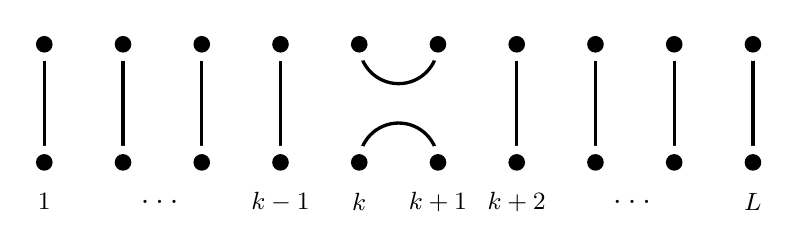
\begin{tikzpicture}
	\foreach \x in {1,2,3,4,7,8,9,10}{
		\draw[very thick] (\x,0) -- (\x,-1.5);}
	\draw[very thick] (5,0) arc (180:360:0.5cm);
	\draw[very thick] (5,-1.5) arc (180:0:0.5cm);
	\foreach \x in {1,...,10} {
		\fill[white] (\x,0) circle (6pt);
		\fill (\x,0) circle (3pt);
		\fill[white] (\x,-1.5) circle (6pt);
		\fill (\x,-1.5) circle (3pt);}
	\draw (1,-2) node[] {\small $1$};
	\draw (2.5,-2) node[] {\large $\dots$};
	\draw (4,-2) node[] {\small $k-1$};
	\draw (5,-2) node[] {\small $k$};
	\draw (6,-2) node[] {\small $k+1$};
	\draw (7,-2) node[] {\small $k+2$};
	\draw (8.5,-2) node[] {\large $\dots$};
	\draw (10,-2) node[] {\small $L$};
\end{tikzpicture}
\end{minipage}
$$
We recall that this is a key point of the Temperley-Lieb algebra, first introduced in \cite{TemperleyLieb}. 
There are also several textbooks
further illuminating the topic, such as \cite{CarterFlathSaito} and \cite{KauffmanLins}, if the interested reader wants to dive deeper.
The reason for the factor of $-2$ multiplying $h^{(1/2)}_{k,k+1}$ on the left-hand-side is that we evaluate the ``bubble'' as $-2$:
$$
\begin{minipage}{1cm}
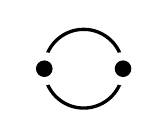
\begin{tikzpicture}
	\draw[very thick] (1,0) arc (180:360:0.5cm);
	\draw[very thick] (1,0) arc (180:0:0.5cm);
	\foreach \x in {1,2} {
		\fill[white] (\x,0) circle (6pt);
		\fill (\x,0) circle (3pt);}
\end{tikzpicture}
\end{minipage}\quad
=\, -2\, .
$$
In turn that is because the down-turned arc represents an un-normalized spin singlet $\ket{\uparrow\downarrow} - \ket{\downarrow\uparrow}$,
but the up-turned arc represents the dual-vector with the spins flipped: $\bra{\downarrow\uparrow} - \bra{\uparrow\downarrow}$.

The basic Temperley-Lieb generators are $U_{k,k+1} = -2h^{(1/2)}_{k,k+1}$,
for $k=1,\dots,L-1$. And the Temperley-Lieb relations are as follows. Firstly,
$$
\forall k,\ell\ \text{ such that }\ |k-\ell|>1\, ,\ \text{ we have }\ U_{k,k+1} U_{\ell,\ell+1}\, =\, U_{\ell,\ell+1} U_{k,k+1}\, .
$$
Secondly, for any $k \in \{1,\dots,L-2\}$ we have
$$
U_{k,k+1} U_{k+1,k+2} U_{k,k+1}\,  =\, U_{k,k+1}\ \text{ and }\ U_{k+1,k+2} U_{k,k+1} U_{k+1,k+2}\,  =\, U_{k+1,k+2}\, .
$$
And finally, for all $k \in \{1,\dots,L-1\}$, we have
$$
U_{k,k+1}^2\, =\, -2 U_{k,k+1}\, .
$$
The diagrams corresponding to the cubic relations are
$$
\begin{minipage}{2cm}
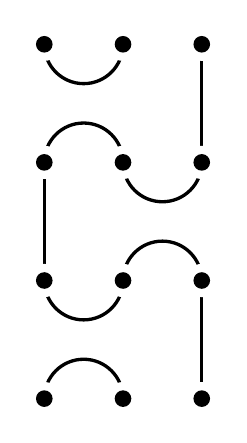
\begin{tikzpicture}
	\draw[very thick] (1,0)  arc (180:360:0.5cm);
	\draw[very thick] (3,0) -- (3,-1.5);
	\draw[very thick] (1,-1.5) arc (180:0:0.5cm);
	\draw[very thick] (2,-1.5)  arc (180:360:0.5cm);
	\draw[very thick] (1,-1.5) -- (1,-3);
	\draw[very thick] (2,-3) arc (180:0:0.5cm);
	\draw[very thick] (1,-3)  arc (180:360:0.5cm);
	\draw[very thick] (3,-3) -- (3,-4.5);
	\draw[very thick] (1,-4.5) arc (180:0:0.5cm);
	\foreach \x in {1,2,3} {
		\fill[white] (\x,0) circle (6pt);
		\fill (\x,0) circle (3pt);
		\fill[white] (\x,-1.5) circle (6pt);
		\fill (\x,-1.5) circle (3pt);
		\fill[white] (\x,-3) circle (6pt);
		\fill (\x,-3) circle (3pt);
		\fill[white] (\x,-4.5) circle (6pt);
		\fill (\x,-4.5) circle (3pt);}
\end{tikzpicture}
\end{minipage}\qquad
=\quad
\begin{minipage}{2cm}
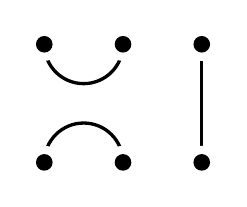
\begin{tikzpicture}
	\draw[very thick] (1,0)  arc (180:360:0.5cm);
	\draw[very thick] (3,0) -- (3,-1.5);
	\draw[very thick] (1,-1.5) arc (180:0:0.5cm);
	\foreach \x in {1,2,3} {
		\fill[white] (\x,0) circle (6pt);
		\fill (\x,0) circle (3pt);
		\fill[white] (\x,-1.5) circle (6pt);
		\fill (\x,-1.5) circle (3pt);}
\end{tikzpicture}
\end{minipage}\qquad \text{ and }\qquad
\begin{minipage}{2cm}
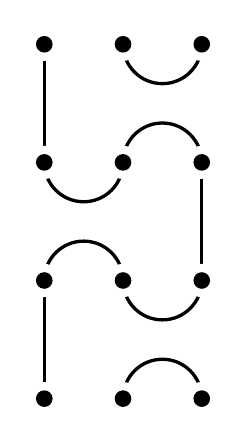
\begin{tikzpicture}[xscale=-1]
	\draw[very thick] (1,0)  arc (180:360:0.5cm);
	\draw[very thick] (3,0) -- (3,-1.5);
	\draw[very thick] (1,-1.5) arc (180:0:0.5cm);
	\draw[very thick] (2,-1.5)  arc (180:360:0.5cm);
	\draw[very thick] (1,-1.5) -- (1,-3);
	\draw[very thick] (2,-3) arc (180:0:0.5cm);
	\draw[very thick] (1,-3)  arc (180:360:0.5cm);
	\draw[very thick] (3,-3) -- (3,-4.5);
	\draw[very thick] (1,-4.5) arc (180:0:0.5cm);
	\foreach \x in {1,2,3} {
		\fill[white] (\x,0) circle (6pt);
		\fill (\x,0) circle (3pt);
		\fill[white] (\x,-1.5) circle (6pt);
		\fill (\x,-1.5) circle (3pt);
		\fill[white] (\x,-3) circle (6pt);
		\fill (\x,-3) circle (3pt);
		\fill[white] (\x,-4.5) circle (6pt);
		\fill (\x,-4.5) circle (3pt);}
\end{tikzpicture}
\end{minipage}\qquad
=\quad
\begin{minipage}{2cm}
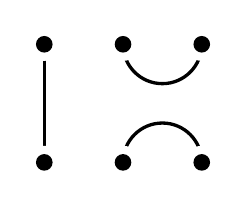
\begin{tikzpicture}[xscale=-1]
	\draw[very thick] (1,0)  arc (180:360:0.5cm);
	\draw[very thick] (3,0) -- (3,-1.5);
	\draw[very thick] (1,-1.5) arc (180:0:0.5cm);
	\foreach \x in {1,2,3} {
		\fill[white] (\x,0) circle (6pt);
		\fill (\x,0) circle (3pt);
		\fill[white] (\x,-1.5) circle (6pt);
		\fill (\x,-1.5) circle (3pt);}
\end{tikzpicture}
\end{minipage}\qquad .
$$
The last diagram in the Temperley-Lieb relations is again an expression that the ``bubble'' evaluates to $-2$:
$$
\begin{minipage}{1cm}

\begin{tikzpicture}
	\draw[very thick] (1,1.5) arc (180:360:0.5cm);
	\draw[very thick] (1,0) arc (180:360:0.5cm);
	\draw[very thick] (1,0) arc (180:0:0.5cm);
	\draw[very thick] (1,-1.5) arc (180:0:0.5cm);
	\foreach \x in {1,2} {
		\fill[white] (\x,0) circle (6pt);
		\fill (\x,0) circle (3pt);
		\fill[white] (\x,-1.5) circle (6pt);
		\fill (\x,-1.5) circle (3pt);
		\fill[white] (\x,1.5) circle (6pt);
		\fill (\x,1.5) circle (3pt);}
\end{tikzpicture}
\end{minipage}\quad
=\, -2\quad 
\begin{minipage}{1cm}

\begin{tikzpicture}
	\draw[very thick] (1,1.5) arc (180:360:0.5cm);
	\draw[very thick] (1,0) arc (180:0:0.5cm);
	\foreach \x in {1,2} {
		\fill[white] (\x,0) circle (6pt);
		\fill (\x,0) circle (3pt);
		\fill[white] (\x,1.5) circle (6pt);
		\fill (\x,1.5) circle (3pt);}
\end{tikzpicture}
\end{minipage}
$$
Aside from the bubble relation, the other relations show that the Temperley-Lieb diagrams may be treated as diagrams following the usual
rules of isotopy.

The reason that this basis is useful in the proof of Theorem \ref{thm:Uniqueness} is that all of the interactions
$$
h_{k,k+1}^{(1/2)}\, =\, -\frac{1}{2} U_{k,k+1}
$$
have non-positive off-diagonal matrix entries in the Hulth\'en bracket basis.
In other words, $U_{k,k+1}$ has nonnegative off-diagonal entries: the only way to get a negative sign is if we multiply by
$-2$ from the bubble relation, but that guarantees that $(k,k+1)$ is some $(a_i,b_i)$. So that would mean that 
$U_{k,k+1} \Theta(\boldsymbol{a},\boldsymbol{b})=-2\Theta(\boldsymbol{a},\boldsymbol{b})$, giving a negative matrix entry,
but only on the diagonal.
Moreover, if all of the coefficients of $h_{1,2}$ to $h_{L-1,L}$ are positive, then the resulting matrix is {\em ergodic}.
By taking a large enough positive constant $C$ and then taking a large enough positive integer $n$,
the matrix power $(C I - h_{1,2}-\dots-h_{L-1,L})^n$ has strictly positive matrix entries.
Then the Perron-Frobenius theorem applies. That was the point of \cite{NSSfoel}.
But now we are also adding in the extra interaction $h_{L,1}$.

The fortunate fact is that this interaction also has a graphical representation in the Hulth\'en bracket basis with a good-sign
condition for the matrix entries. But this is only true if we consider the singlet sector, where the Hulth\'en bracket basis
is labelled by non-crossing perfect matchings, with no sites unpaired. The graph is somewhat ungainly, but is shown below:
we call it $\widetilde{U}_{L,1}$.
$$
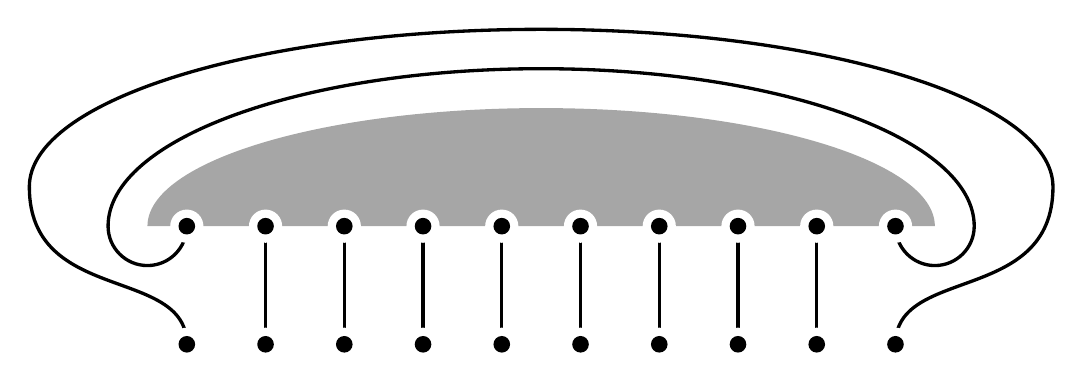
\begin{tikzpicture}
	\foreach \x in {2,3,...,9}{
		\draw[very thick] (\x,0) -- (\x,-1.5);}
	\fill[black!35!white] (0.5,0) -- (10.5,0) arc (0:180:5cm and 1.5cm);
	\draw[very thick] (1,0) arc (360:180:0.5cm) arc (180:0:5.5cm and 2cm) arc (360:180:0.5cm);
	\draw[very thick] (1,-1.5) .. controls (1,-0.5) and (-1,-1) .. (-1,0.5) arc (180:0:6.5cm and 2cm) .. controls (12,-1) and (10,-0.5) .. (10,-1.5);
	\foreach \x in {1,...,10} {
		\fill[white] (\x,0) circle (6pt);
		\fill (\x,0) circle (3pt);
		\fill[white] (\x,-1.5) circle (6pt);
		\fill (\x,-1.5) circle (3pt);}
\end{tikzpicture}
$$
The gray arc region is supposed to indicate the region that all of the arcs forming the perfect matching will be constrained to.
We may alway continuously deform any non-crossing perfect matching so that all the edges are contained in the gray region.
Then the arcs for $\widetilde{U}_{L,1}$ may be drawn so as to not intersect the gray region where all the other arcs are already
drawn. At that point one uses the usual isotopy reduction to simplify the resulting graphical representation of a vector.

Let us consider two examples:

\begin{equation*}
\begin{split}
&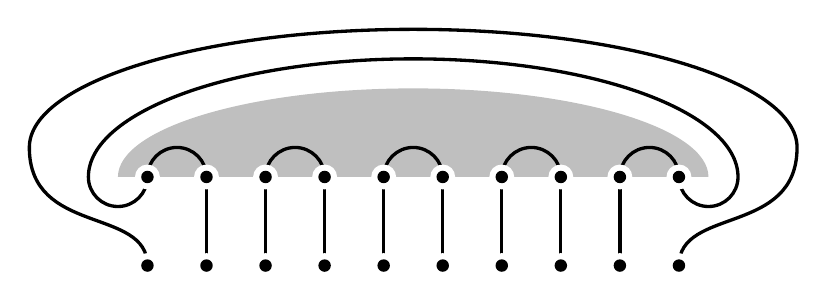
\begin{tikzpicture}[xscale=0.75,yscale=0.75]
	\foreach \x in {2,3,...,9}{
		\draw[very thick] (\x,0) -- (\x,-1.5);}
	\fill[black!25!white] (0.5,0) -- (10.5,0) arc (0:180:5cm and 1.5cm);
	\foreach \x in {1,3,...,9}{
		\draw[very thick] (\x,0) arc (180:0:0.5cm);}
	\draw[very thick] (1,0) arc (360:180:0.5cm) arc (180:0:5.5cm and 2cm) arc (360:180:0.5cm);
	\draw[very thick] (1,-1.5) .. controls (1,-0.5) and (-1,-1) .. (-1,0.5) arc (180:0:6.5cm and 2cm) .. controls (12,-1) and (10,-0.5) .. (10,-1.5);
	\foreach \x in {1,...,10} {
		\fill[white] (\x,0) circle (6pt);
		\fill (\x,0) circle (3pt);
		\fill[white] (\x,-1.5) circle (6pt);
		\fill (\x,-1.5) circle (3pt);}
\end{tikzpicture}\\[10pt]
&\hspace{3cm} =\,
\raisebox{0.5cm}{
\begin{minipage}{8cm}
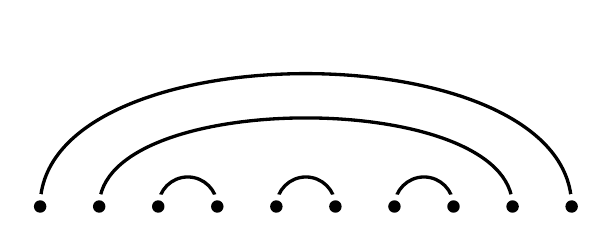
\begin{tikzpicture}[xscale=0.75,yscale=0.75]
%	\foreach \x in {2,3,...,9}{
%		\draw[very thick] (\x,0) -- (\x,-1.5);}
%	\fill[black!35!white] (0.5,0) -- (10.5,0) arc (0:180:5cm and 1.5cm);
	\foreach \x in {3,5,7}{
		\draw[very thick] (\x,0) arc (180:0:0.5cm);}
	\draw[very thick] (2,0) .. controls (2,2) and (9,2) .. (9,0);
	\draw[very thick] (1,0) .. controls (1,3) and (10,3) .. (10,0);
	\foreach \x in {1,...,10} {
		\fill[white] (\x,0) circle (6pt);
		\fill (\x,0) circle (3pt);}
\end{tikzpicture}
\end{minipage}}
\end{split}
\end{equation*}
and
\begin{equation*}
\begin{split}
&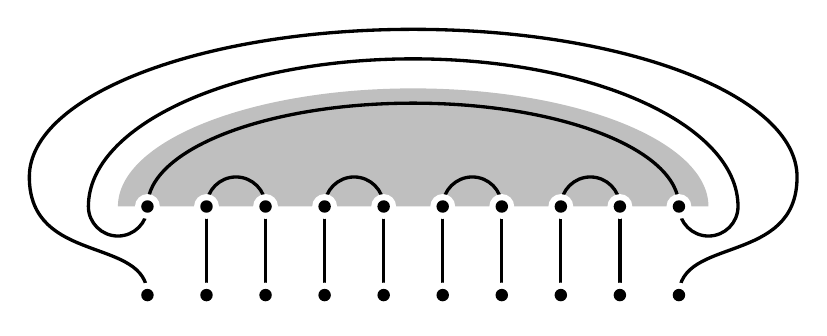
\begin{tikzpicture}[xscale=0.75,yscale=0.75]
	\foreach \x in {2,3,...,9}{
		\draw[very thick] (\x,0) -- (\x,-1.5);}
	\fill[black!25!white] (0.5,0) -- (10.5,0) arc (0:180:5cm and 2cm);
	\foreach \x in {2,4,...,8}{
		\draw[very thick] (\x,0) arc (180:0:0.5cm);}
	\draw[very thick] (1,0) arc (180:0:4.5cm and 1.75cm);
	\draw[very thick] (1,0) arc (360:180:0.5cm) arc (180:0:5.5cm and 2.5cm) arc (360:180:0.5cm);
	\draw[very thick] (1,-1.5) .. controls (1,-0.5) and (-1,-1) .. (-1,0.5) arc (180:0:6.5cm and 2.5cm) .. controls (12,-1) and (10,-0.5) .. (10,-1.5);
	\foreach \x in {1,...,10} {
		\fill[white] (\x,0) circle (6pt);
		\fill (\x,0) circle (3pt);
		\fill[white] (\x,-1.5) circle (6pt);
		\fill (\x,-1.5) circle (3pt);}
\end{tikzpicture}\\[10pt]
&\hspace{3cm} =\, -2 
\raisebox{0.5cm}{
\begin{minipage}{8cm}
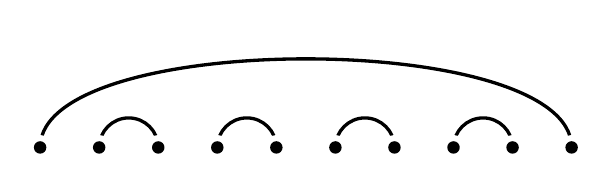
\begin{tikzpicture}[xscale=0.75,yscale=0.75]
%	\foreach \x in {2,3,...,9}{
%		\draw[very thick] (\x,0) -- (\x,-1.5);}
%	\fill[black!35!white] (0.5,0) -- (10.5,0) arc (0:180:5cm and 1.5cm);
	\foreach \x in {2,4,...,8}{
		\draw[very thick] (\x,0) arc (180:0:0.5cm);}
	\draw[very thick] (1,0) .. controls (1,2) and (10,2) .. (10,0);
	\foreach \x in {1,...,10} {
		\fill[white] (\x,0) circle (6pt);
		\fill (\x,0) circle (3pt);}
\end{tikzpicture}
\end{minipage}}
\end{split}
\end{equation*}
where the factor of $-2$ is because of the ``bubble.''
(We very much use the fact that we are using the isotropic Heisenberg model, where the parameter $q$
which would control the anisotropy in the XXZ model is set equal to $q=1$.
That is necessary for being able to turn the arcs around in pairs because each reversal only
picks up a sign of $-1$. So the usual ``bubble'' factor $-[2]_q$ is just $-2$.)

Note that in the second example, we get a negative sign for the matrix entry of $\widetilde{U}_{L,1}$.
But that is a diagonal matrix entry. For the same reason as before, all the off-diagonal matrix entries of $\widetilde{U}_{L,1}$ 
are nonnegative.
Therefore, since $h_{L,1}^{(1/2)} = -\frac{1}{2} \widetilde{U}_{L,1}$ in the Hulth\'en bracket basis,
we see that
$$
H^{\mathrm{FM}}_{1/2,L}\, =\, h_{1,2}^{(1/2)} + \dots + h_{L-1,L}^{(1/2)} + h_{L,1}^{(1/2)}
$$
still has the good-signs condition: all off-diagonal matrix entries are non-positive in the Hulth\'en bracket basis.
The ergodicity property is not negatively affected by adding one more interaction with the good-signs condition.
Therefore, the Perron-Frobenius theorem applies, as it did in the cited reference.

We conclude that in the singlet sector, which is the span of the Hulth\'en bracket basis for non-crossing, perfect matchings
(with no unpaired spin sites), there is a unique ground state vector of $H^{\mathrm{FM}}_{1/2,L}$ restricted to this 
invariant subspace. Moreover, that vector is positive in the Hulth\'en bracket basis.
Consider the two basis vectors corresponding to the graphical representations we used as the last two examples:
\begin{equation*}
\begin{split}
\begin{minipage}{9cm}

\begin{tikzpicture}[xscale=0.75,yscale=0.75]
	\foreach \x in {1,3,...,9}{
		\draw[very thick] (\x,0) arc (180:0:0.5cm);}
	\foreach \x in {1,...,10} {
		\fill[white] (\x,0) circle (6pt);
		\fill (\x,0) circle (3pt);}
\end{tikzpicture}
\end{minipage}\\ 
&\hspace{-3cm} =\, - T
\raisebox{0.5cm}{
\begin{minipage}{8cm}
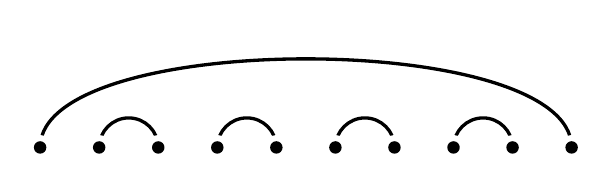
\begin{tikzpicture}[xscale=0.75,yscale=0.75]
%	\foreach \x in {2,3,...,9}{
%		\draw[very thick] (\x,0) -- (\x,-1.5);}
%	\fill[black!35!white] (0.5,0) -- (10.5,0) arc (0:180:5cm and 1.5cm);
	\foreach \x in {2,4,...,8}{
		\draw[very thick] (\x,0) arc (180:0:0.5cm);}
	\draw[very thick] (1,0) .. controls (1,2) and (10,2) .. (10,0);
	\foreach \x in {1,...,10} {
		\fill[white] (\x,0) circle (6pt);
		\fill (\x,0) circle (3pt);}
\end{tikzpicture}
\end{minipage}}
\end{split}
\end{equation*}
Here $T$ is the translation operator by 1 unit say to the right.
(Note that both of these matchings are invariant under the square of translation $T^2$. They are 2-periodic.)
Because the spin singlet creation operator is $S^-_{b_r} - S^-_{a_r}$ when we span an arc across the boundary and turn it around
either going from $(L-1,L)$ to $(1,L)$ after application of $T$ the order of the $a_r$ and $b_r$ are reversed for that pair responsible
for the spin singlet creation operator for the arc which spans $(1,L)$ in one of the two basis elements.
That is why we get $-T$. But since both coefficients must be positive, that means that $T \Psi^{\mathrm{FM}}_{\min}(0) = -\Psi^{\mathrm{FM}}_{\min}(0)$ (as opposed to the other alternative of being translation invariant, which is the only other
alternative when the eigenvector is non-degenerate since $H^{\mathrm{FM}}_{\min}$ has real matrix entries).

This concludes the proof of the lemma for the special case of $j=1/2$.
But there are higher spin versions of the Hulth\'en bracket basis and the Templerley-Lieb algebra.
Essentially, the extra element is the Jones-Wenzl projectors (represented by boxes).
But let us leave all extra details as an exercise for the interested reader, who can follow the lead in reference \cite{NachtergaeleStarr}.
The only detail not covered there is what happens if one translates to determine the translation eigenvalues.
Essentially, one is translating $2j$ units because one must translate full Jones-Wenzl operators which take $2j$
spin sites as their inputs and outputs. That is why we get the formula stated in the lemma.

For example, for $j=1$, the diagrammatic picture of the analogous formula as the preceding displayed equation is as follows:
\begin{equation*}
\begin{split}
\begin{minipage}{9cm}
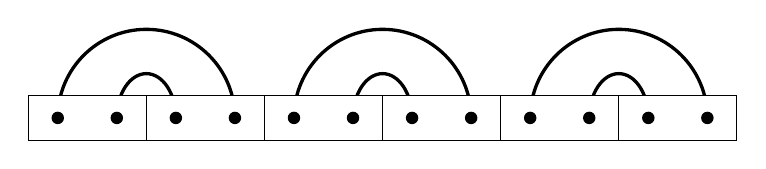
\begin{tikzpicture}[xscale=0.75,yscale=0.75]
\foreach \x in {1,5,9} {
		\draw[very thick] (\x,0) arc (180:0:1.5cm);
		\draw[very thick] (\x+1,0) arc (180:0:0.5cm and 0.75cm);}
\foreach \x in {1,3,5,7,9,11} {
		\filldraw[fill=white] (\x-0.5,-0.375) rectangle (\x+1.5,0.375);}
\foreach \x in {1,...,12} {
		\fill[white] (\x,0) circle (6pt);
		\fill (\x,0) circle (3pt);}
\end{tikzpicture}
\end{minipage}\\[15pt]
&\hspace{-5cm} =\, T\
\raisebox{0.5cm}{
\begin{minipage}{9cm}
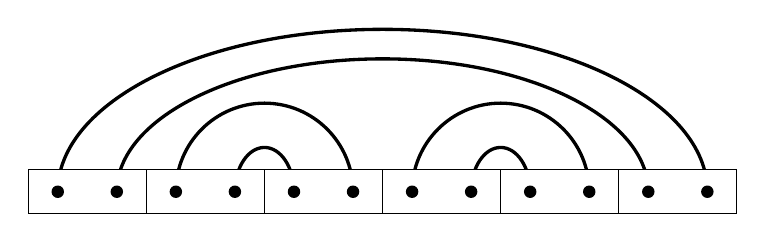
\begin{tikzpicture}[xscale=0.75,yscale=0.75]
\draw[very thick] (1,0) arc (180:0:5.5cm and 2.75cm); 
\draw[very thick] (2,0) arc (180:0:4.5cm and 2.25cm); 
\foreach \x in {3,7} {
		\draw[very thick] (\x,0) arc (180:0:1.5cm);
		\draw[very thick] (\x+1,0) arc (180:0:0.5cm and 0.75cm);}
\foreach \x in {1,3,5,7,9,11} {
		\filldraw[fill=white] (\x-0.5,-0.375) rectangle (\x+1.5,0.375);}
\foreach \x in {1,...,12} {
		\fill[white] (\x,0) circle (6pt);
		\fill (\x,0) circle (3pt);}
\end{tikzpicture}
\end{minipage}}\qquad .
\end{split}
\end{equation*}

\begin{remark}
The same method clearly does not work for spins other than $S=0$. The reason is that there are unpaired spin sites:
the Hulth\'en brackets do not form a perfect matching. Therefore, there would be crossings
and the resolution 
$\raisebox{0cm}{\begin{minipage}{0.25cm}
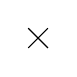
\begin{tikzpicture} \draw (0,0) -- (0.25,-0.25); \draw (0,-0.25) -- (0.25,0);
\end{tikzpicture}
\end{minipage}}
 = 
\raisebox{0cm}{\begin{minipage}{0.25cm}
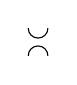
\begin{tikzpicture} \draw (0,0) arc (180:360:0.125cm); \draw (0,-0.35) arc (180:0:0.125cm); 
\end{tikzpicture}
\end{minipage}}\
+\
\raisebox{0cm}{\begin{minipage}{0.25cm}
\begin{tikzpicture} \draw (0,0) -- (0,-0.25); \draw (0.25,0) -- (0.25,-0.25); 
\end{tikzpicture}
\end{minipage}}
$
introduces the potential to have negative off-diagonal entries because 
$\raisebox{0cm}{\begin{minipage}{0.25cm}
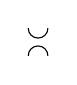
\begin{tikzpicture} \draw (0,0) arc (180:360:0.125cm); \draw (0,-0.35) arc (180:0:0.125cm); 
\end{tikzpicture}
\end{minipage}}$ can give rise to bubbles which multiply the diagram by $-2$.
Of course, when $j=1/2$, we also expect a 2-fold degeneracy of the minimum energy eigenstates among spin $S$ for $0<S<L/2$.
So the Perron-Frobenius theorem should not apply to those cases.
\end{remark}

\subsection{Two-fold multiplicity of pure Bloch wall states}

% Figure environment removed

Dhar and Shastry proposed Bloch wall vectors as approximations to $\Psi^{\mathrm{FM}}_{\min}(S;j,L)$ when $(jL-S)/L<1/4$.
(So the Bloch walls are applicable when the density of ``spin deviates'' is less than $1/4$.)
Let us denote vectors $\Xi_{\ell}(S;j,L)$ as
\begin{equation*}
	\Xi_{\ell}(S;j,L)\, =\, \left(\widehat{S}^{-}_{\ell}\right)^{jL-S} \Big(\Psi_{j,j} \otimes \cdots \otimes \Psi_{j,j}\Big)\, .
\end{equation*}
Then Dhar and Shastry's proposal for the Bloch wall vectors are $\Xi_{1}(S;j,L)$ for $S>(j-\frac{1}{4})L$.
But they could equally well have chosen the complex conjugate eigenvector $\Xi_{-1}(S;j,L)$.
Let us note that for $j=1/2$, we have for the inner-product, setting $K=jL-S$, 
\begin{equation*}
\begin{split}
	\langle \Xi_{m}(S;1/2,L)\, ,\ \Xi_{\ell}(S;1/2,L)\rangle\,
	&=\, (K!)^2 \sum_{\substack{1\leq x(1)<\dots<x(K)\leq L\\
1\leq y(1)<\dots<y(K)\leq L}}
q_1^{x(1)+\dots+x(K)} q_2^{y(1)+\dots+y(K)}\\
&\hspace{-1cm} \cdot \langle (S_{x(1)}^- \cdots S_{x(K)}^-)\Omega_L\, ,\
(S_{y(1)}^- \cdots S_{y(K)}^-)\Omega_L\rangle\, ,
\end{split}
\end{equation*}
for $q_1=\exp(-2\pi i m/L)$, $q_2=\exp(2\pi i \ell/L)$ and 
where the inner-product is non-zero if and only if $x(k)=y(k)$ for all $k \in \{1,\dots,K\}$.
Therefore, we obtain the $q$-binomial
\begin{equation*}
	\langle \Xi_{m}(S;1/2,L)\, ,\ \Xi_{\ell}(S;1/2,L)\rangle\,
	=\, (K!)^2 
\left[\begin{matrix}L \\ K\end{matrix}\right]_q q^{K(K+1)/2} \Bigg|_{\substack{q=\exp(2\pi i (\ell-m)/L)\\K=(L/2)-S}}\, .
\end{equation*}
Since $q$ is a root-of-unity, the $q$-Lucas theorem applies, for example from \cite{KlugeRubey} Lemma 3.1,
$$
\left[\begin{matrix}L \\ K\end{matrix}\right]_q\, =\, \binom{\lfloor L/R \rfloor}{\lfloor K/R \rfloor}\cdot
\left[\begin{matrix}L - R \lfloor L/R \rfloor\\ K - R\lfloor K/R \rfloor \end{matrix}\right]_q\, ,\
\text{ for }\ R=\min(\{r \in \{1,2,\dots\}\, :\, q^r=1\})\, .
$$
If $K<R$ then the inner-product turns out to be $0$ because $[L]_q!/[L-K]_q!$ has a factor $[L]_q$ which is 0
(since $q^L=0$) but $[K]_q!$ is not $0$. This is also necessitated by consideration of translation eigenvalues.

If $K=R$ then the $q$-binomial coefficient on the right-hand-side of the formula above equals 1.
In particular, taking $\ell=1$ and $m=-1$, and taking $S=0$, so that $R=K=L/2$, we see that the cosine of the angle between the two vectors is 
exponentially small, of the order $2^{-L/2}$ at the exponential level.
So the two vectors that one obtains by taking $\Xi_{1}(0;1/2,L)$ and $\Xi_{-1}(0;1/2,L)$
are almost orthogonal.
Since they both have the same energy expectation, neither one can be the eigenvector with minimum
energy in the spin-singlet sector.
That is because of uniqueness of that vector, Theorem \ref{thm:Uniqueness}.



We remind the readers that this is consistent with Dhar and Shastry's conclusion that the Bloch wall approximations cease to be good approximations
when $S/L<j-\frac{1}{4}$, meaning $jL-S>L/4$. This includes $S=0$.
\begin{remark}
Despite the fact that Bloch wall vectors themselves appear to lose validity when $S/L<j-\frac{1}{4}$, the energy approximation seems reasonably accurate up to the level that we can see.
For example, for $L=20$, we have plotted the actual data against the approximation in Figure \ref{fig:BlochWallApprox}.
It is possible that the corrections are of higher order than the lowest order we have looked for in the numerics.
\end{remark}


The same type of conclusion holds if $j>1/2$ by using a ``spin-ladder'' representation, that we do not describe here.
Suffice it to say that the cosine of the angle between  $\Xi_{1}(0;j,L)$ and $\Xi_{-1}(0;j,L)$
is even smaller than $|\langle \Xi_{1}(0;1/2,L),\Xi_{1}(0;1/2,L)\rangle|^{2j} \|\Xi_{1}(0;1/2,L)\|^{-2j} \|\Xi_{-1}(0;1/2,L)\|^{-2j}$
if $j>1/2$. (It is a convex combination of this quantity and numerous other $0$'s.)
Or we could say
$$
	\lim_{L \to \infty} L^{-1}\, \ln\left(\frac{|\langle \Xi_{1}(0;1/2,L),\Xi_{1}(0;1/2,L)\rangle|}{\|\Xi_{1}(0;1/2,L)\| \cdot
\|\Xi_{-1}(0;1/2,L)\|}\right)\, =\, -j \ln(2)\, .
$$
What seems likely is that some correction to the basic Bloch wave structure, perhaps with a linear combination of the two states,
gives the actual $\Psi^{\mathrm{FM}}_{\min}(0;j,L)$. 
We note that in other areas of condensend matter physics, such as correlated electron systems, 
corrections to pure Slater determinants take the form of Jastrow factors.
Here, we do not need to guess what is the correct form because the Bethe ansatz applies
and Sutherland has already calculated the exact ground state.
If necessary, one should be able to extrapolate from that form to higher spin $j>1/2$.

% Figure environment removed


Numerically, in the spin singlet sector there seems to be a larger-than-usual gap at the bottom of the spectrum of the ferromagnet.
But there are other momentum-$\pi$ states with total spin $1$, $2$, and so on.
So a linear combination of $\Xi_{1}(0;1/2,L)$ and $\Xi_{-1}(0;1/2,L)$, perhaps with a Jastrow-like factor multiplied,
may give the spin singlet $\Psi^{\mathrm{FM}}_{\min}(0;j,L)$.
And a different combination may give the lowest momentum-$\pi$ state with spin-1, for example.
This proposal is motivated by the plots of actual eigenvalues using the Lanczos iteration algorithm.
For example, see Figure \ref{fig:Dodecagon} for an example with $j=1/2$ and $L=12$.

We will discuss the spin of the pure Bloch waves at the beginning of the next section.

\section{The SMA part 1: consideration of the denominator}

In the single mode approximation (SMA) we consider $\langle \Phi_{\ell}\, ,\ H^{\mathrm{FM}}_{j,L} \Phi_{\ell}\rangle$
where $\Phi_{\ell} = \widehat{S}^+_{\ell} \Psi^{\mathrm{FM}}(0;j,L)$.
Since $\Psi^{\mathrm{FM}}(0;j,L)$ is the lowest energy eigenstate of 
$H^{\mathrm{FM}}_{j,L}$ among all spin singlets, and it is unique this means it has a particular property.
For any unitary operator which is a symmetry of the Hamiltonian, we must have the property that $\Psi^{\mathrm{FM}}(0;j,L)$  is also an eigenvector of that unitary.
Using the eigenvector property, the calculation of $\langle \Phi_{\ell}\, ,\ H^{\mathrm{FM}}_{j,L} \Phi_{\ell}\rangle$
can be reduced to calculating certain commutators.
Using the symmetry property, it amounts to calculation of a double-commutator.
That is familiar in perturbation theory, for example from the Duhamel two-point function (DTF).
(See, for example,  \cite{DLS} for an application of the DTF.)
We start with the single commutator.
% Figure environment removed

But first, let us review a different topic.
We are considering a Rayleigh quotient:
$$
\frac{\langle \Psi^{\mathrm{FM}}_{\min}(0;j,L)\, ,\ \widehat{S}^-_{-\ell} H_{j,L}^{\mathrm{FM}} 
\widehat{S}^+_{\ell} \Psi^{\mathrm{FM}}_{\min}(0;j,L)\rangle}
{\|\widehat{S}^+_{\ell} \Psi^{\mathrm{FM}}_{\min}(0;j,L)\|^2}\, .
$$
By the variational principle, this provides an upper bound for $\widetilde{E}^{\mathrm{FM}}_{\min}\left(1,e^{i\theta} e^{2\pi i \ell/L};j,L\right)$ which in turn is an upper bound for $E^{\mathrm{FM}}_{\min}(0;j,L)$.
Moreover, in this section we will show how to simplify the numerator, which we have called $\mathcal{H}(\ell;j,L)$.
More precisely, we are able to simplify the quantity
$$
\Delta \mathcal{H}(\ell;j,L)\, 
=\, \left\langle \Psi^{\mathrm{FM}}_{\min}(0)\, ,\  \widehat{S}^-_{-\ell} 
\left(H^{\mathrm{FM}}_{j,L}-E^{\mathrm{FM}}_{\min}(0;j,L)\right) 
\widehat{S}^+_{\ell}  \Psi^{\mathrm{FM}}_{\min}(0)\right\rangle\, .
$$
But this leaves the denominator which still requires consideration since
$$
\widetilde{E}^{\mathrm{FM}}_{\min}\left(1,e^{i\theta} e^{2\pi i \ell/L};j,L\right) - E^{\mathrm{FM}}_{\min}(0;j,L)\, 
\leq\, \frac{\Delta \mathcal{H}(\ell;j,L)}{\|\widehat{S}^+_{\ell} \Psi^{\mathrm{FM}}_{\min}(0;j,L)\|^2}\, .
$$ 
We call the denominator $\mathcal{Z}(\ell;j,L)$. It is a kind of structure factor for $\Psi^{\mathrm{FM}}_{\min}(0;j,L)$.
%Another possible structure factor would be $\left\|\sum_{\alpha=1}^{L} e^{2\pi i \alpha \ell/L} S^{(3)}_{\alpha} \Psi^{\mathrm{FM}}_{\min}(0;j,L)\right\|^2$. That equals $\frac{1}{2} \mathcal{Z}(\ell;j,L)$ by symmetry considerations.
%(By symmetry it is the same as $\left\|\sum_{\alpha=1}^{L} e^{2\pi i \alpha \ell/L} S^{(1)}_{\alpha} \Psi^{\mathrm{FM}}_{\min}(0;j,L)\right\|^2$, which is $1/4$ times $\|\widehat{S}^+_{\ell} \Psi^{\mathrm{FM}}_{\min}(0;j,L)\|^2+\|\widehat{S}^-_{\ell} \Psi^{\mathrm{FM}}_{\min}(0;j,L)\|^2$ due to orthogonality. By symmetry both summands are equal.)


What we do is simply to numerically calculate $\mathcal{Z}(\ell;j,L)$. It is clear that it is nonnegative.
See Figure \ref{fig:StructureFactor} for an example, when $L=20$ and $j=1/2$.
Because
\begin{equation*}
	\mathcal{Z}(\ell;j,L)\, 
=\, \left\langle \Psi^{\mathrm{FM}}_{\min}(0)\, ,\ \widehat{S}^-_{-\ell} \widehat{S}^+_{\ell}
 \Psi^{\mathrm{FM}}_{\min}(0)\right\rangle\,
=\, \sum_{\alpha=1}^{L} \sum_{\beta=1}^{L} e^{2\pi i \ell (\alpha-\beta)/L} 
\left\langle \Psi^{\mathrm{FM}}_{\min}(0)\, ,\ {S}^-_{\beta} {S}^+_{\alpha}
 \Psi^{\mathrm{FM}}_{\min}(0)\right\rangle\, ,
\end{equation*}
we have
\begin{equation*}
\begin{split}
	\sum_{\ell=1}^{L} \mathcal{Z}(\ell;j,L)\, 
&=\, \sum_{\alpha=1}^{L} \sum_{\beta=1}^{L} \left(\sum_{\ell=1}^{L} e^{2\pi i \ell (\alpha-\beta)/L} \right)
\left\langle \Psi^{\mathrm{FM}}_{\min}(0)\, ,\ {S}^-_{\beta} {S}^+_{\alpha}
 \Psi^{\mathrm{FM}}_{\min}(0)\right\rangle\\
&=\, \sum_{\alpha=1}^{L} \sum_{\beta=1}^{L} \left(L \delta_{\alpha,\beta} \right)
\left\langle \Psi^{\mathrm{FM}}_{\min}(0)\, ,\ {S}^-_{\beta} {S}^+_{\alpha}
 \Psi^{\mathrm{FM}}_{\min}(0)\right\rangle\\
&=\, L \sum_{\alpha=1}^{L}  
\left\langle \Psi^{\mathrm{FM}}_{\min}(0)\, ,\ {S}^-_{\alpha} {S}^+_{\alpha}
 \Psi^{\mathrm{FM}}_{\min}(0)\right\rangle\, .
\end{split}
\end{equation*}
For spin-$1/2$ this equals $L$ times 
$\left\langle \Psi^{\mathrm{FM}}_{\min}(0;1/2,L)\, ,\ (S_{\mathrm{tot}}^{(3)}+\frac{1}{2} L \cdot \mathbbm{1})
 \Psi^{\mathrm{FM}}_{\min}(0;1/2,L)\right\rangle$.
But by $\mathrm{SU}(2)$ symmetry, we have $S_{\mathrm{tot}}^{(3)}\Psi^{\mathrm{FM}}_{\min}(0;1/2,L)=0$.
Therefore, we have
\begin{equation*}
	\sum_{\ell=1}^{L} \mathcal{Z}(\ell;j,L)\, 
=\, \frac{L^2}{2} \|\Psi^{\mathrm{FM}}_{\min}(0)\|^2\, =\, \frac{L^2}{2}\, ,
\end{equation*}
assuming that $\Psi^{\mathrm{FM}}_{\min}(0)$ is normalized.

Note that $T$ is a symmetry of $H^{\mathrm{FM}}_{j,L}$ on the ring $\mathbb{Z}/L\mathbb{Z}$.
Therefore, $\Psi^{\mathrm{FM}}_{\min}(0)$ is a $T$ eigenvector.
By the previous lemma we know the translation eigenvalue is $(-1)^{2j}$.
But in particular, this means that $\langle \Psi^{\mathrm{FM}}_{\min}(0;j,L)\, ,\ \widehat{S}^-_{-\ell}
\widehat{S}^+_{m} \Psi^{\mathrm{FM}}_{\min}(0;j,L)\rangle$ will be non-zero only if $\ell=m$ (modulo $L$).
That is because conjugating $\widehat{S}^{-}_{-\ell} \widehat{S}^+_{m}$ gives 1 only if $\ell=m$ (modulo $L$).
But applying $T$ to $\ket{\Psi^{\mathrm{FM}}_{\min}(0;j,L)}$ and $\bra{\Psi^{\mathrm{FM}}_{\min}(0;j,L)}$ yields multiplication
by the $T$ eigenvalue and its conjugate, respectively, which multiply to $1$. So if $\ell\neq m$ modulo $L$ the only
way to have equality of the two numbers is if $\langle \Psi^{\mathrm{FM}}_{\min}(0;j,L)\, ,\ \widehat{S}^-_{-\ell}
\widehat{S}^+_{m} \Psi^{\mathrm{FM}}_{\min}(0;j,L)\rangle=0$.
(This is the usual orthogonality of eigenvector for different eigenvalues argument for Hermitian and unitary operators.)

Similarly, since $\sum_{\ell=1}^{L} \cos(2\pi \ell/L) e^{2\pi i \ell(\alpha-\beta)}$ equals $L/2$ times $\delta_{\beta,\alpha+1} +\delta_{\beta,\alpha-1}$, we have
$$
\sum_{\ell=1}^{L} \cos(2\pi \ell/L)\mathcal{Z}(\ell;j,L)\,
=\, L \sum_{\alpha=1}^{L} \left\langle \Psi^{\mathrm{FM}}_{\min}(0)\, ,\ \frac{{S}^-_{\alpha} {S}^+_{\alpha+1}
+{S}^-_{\alpha+1} {S}^+_{\alpha}}{2}\, 
 \Psi^{\mathrm{FM}}_{\min}(0)\right\rangle\, .
$$
But this is also equal to 
$$
\sum_{\ell=1}^{L} \cos(2\pi \ell/L) \mathcal{Z}(\ell;j,L)\,
=\, L \sum_{\alpha=1}^{L} \left\langle \Psi^{\mathrm{FM}}_{\min}(0)\, ,\ \big({S}^{(1)}_{\alpha} {S}^{(1)}_{\alpha+1}
+{S}^{(2)}_{\alpha} {S}^{(2)}_{\alpha+1}\big)\, 
 \Psi^{\mathrm{FM}}_{\min}(0)\right\rangle\, .
$$
And by $\mathrm{SU}(2)$ symmetry of $\Psi^{\mathrm{FM}}_{\min}(0)$, this equals
$$
\sum_{\ell=1}^{L} \cos(2\pi \ell/L) \mathcal{Z}(\ell;j,L)\,
=\, \frac{2 L}{3} \sum_{\alpha=1}^{L} \left\langle \Psi^{\mathrm{FM}}_{\min}(0)\, ,\ \big({S}^{(1)}_{\alpha} {S}^{(1)}_{\alpha+1}
+{S}^{(2)}_{\alpha} {S}^{(2)}_{\alpha+1}
+{S}^{(3)}_{\alpha} {S}^{(3)}_{\alpha+1}\big)\, 
 \Psi^{\mathrm{FM}}_{\min}(0)\right\rangle\, .
$$
So we have
$$
\sum_{\ell=1}^{L} \cos(2\pi \ell/L) \mathcal{Z}(\ell;j,L)\,
=\, \frac{2 L}{3} \sum_{\alpha=1}^{L} \left\langle \Psi^{\mathrm{FM}}_{\min}(0)\, ,\ \big(-H_{j,L}^{\mathrm{FM}}
+j^2L\cdot \mathbbm{1}\big)\,
 \Psi^{\mathrm{FM}}_{\min}(0)\right\rangle\, .
$$
In other words,
$$
\sum_{\ell=1}^{L} \cos(2\pi \ell/L) \mathcal{Z}(\ell;j,L)\,
=\, \frac{2 L}{3}\, \big(-E^{\mathrm{FM}}_{\min}(0;j,L)+j^2L\big)\, ,
$$
assuming that $\Psi^{\mathrm{FM}}_{\min}(0)$ is normalized.

According to the numerical figure, we may see that one possibility is $\mathcal{Z}(\ell;1/2,L) \approx \frac{L}{3} + \frac{L^2}{12} \left(\delta_{\ell,1}+\delta_{\ell,-1}\right)$.
This is not exactly right because $\mathcal{Z}(0;1/2,L)=0$ since $\widehat{S}^+_0 \Psi^{\mathrm{FM}}_{\min}(0)$
equals $S^+_{\mathrm{tot}} \Psi^{\mathrm{FM}}_{\min}(0)$, which is $0$ by $\mathrm{SU}(2)$ symmetry (the singlet property)
of $\Psi^{\mathrm{FM}}_{\min}(0)$. But that is a lower-order correction. If we took it into account, we might guess that
$\mathcal{Z}(\ell;1/2,L) \approx \frac{L}{3} \big(1-\delta_{\ell,0}-\delta_{\ell,1}-\delta_{\ell,-1}\big) 
+ \frac{L(L+6)}{12} \big(\delta_{\ell,1}+\delta_{\ell,-1}\big)$.
{\em This is just a guess based on some numerical evidence.} Clearly it is not exact, as we can see in Figure \ref{fig:StructureFactor}.

\subsection{The structure factor in the pure Bloch wall ansatz}

It is approximately as simple to calculate the structure factor in the pure Bloch wall ansatz 
as it is to calculate the inner-product of two Bloch wall vectors, which we did in the last section.
Here we restrict attention to $j=1/2$ (for simplicity).
By direct calculation, writing $K$ for $L/2$, we have
$$
	\widehat{S}^+_m \cdot \Xi_{\ell}(0;1/2,L)\, =\, K!\, \sum_{1\leq y_1<\dots<y_{K-1}\leq L} 
q_{\ell}^{y_{1}+\dots+y_{K-1}}
\sum_{x \in \{y_1,\dots,y_{K-1}\}^C} q_{m+\ell}^x
\left(\prod_{k=1}^{K-1} S_{y_k}^-\right) \Omega_L\, ,
$$
where $q_{\ell} = \exp(2\pi i \ell/L)$ for each $\ell$. If $m+\ell \equiv 0\ (\operatorname{mod} L)$ 
this reduces to $K(L-K+1) \Xi_{\ell}(1;1/2,L)$. So
$$
\frac{\|\widehat{S}^+_{-\ell}\cdot \Xi_{\ell}(0;1/2,L)\|^2}{\|\Xi_{\ell}(0;1/2,L)\|^2}\, 
=\, K(L-K+1)\, =\, \frac{L}{2} \left(\frac{L}{2}+1\right)\, .
$$
If $m+\ell\not\equiv 0\, (\operatorname{mod} L)$ then $\sum_{x=1}^{L} q_{m+\ell}^x=0$ so
$$
	\widehat{S}^+_m \cdot \Xi_{\ell}(0;1/2,L)\, =\, -K!\, \sum_{1\leq y_1<\dots<y_{K-1}\leq L} q_{\ell}^{y_1+\dots+y_{K-1}}
\sum_{k=1}^{K-1} q_{m+\ell}^{y_k}
\left(\prod_{k=1}^{K-1} S_{y_k}^-\right) \Omega_L\, ,
$$
From this, in the latter case, we have that
$$
\|\widehat{S}^+_m \cdot \Xi_{\ell}(0;1/2,L)\|^2\, =\, (K!)^2 \sum_{1\leq y_1<\dots<y_{K-1}\leq L} 
\sum_{k=1}^{K-1} \sum_{k'=1}^{K-1} q_{\ell+m}^{y_k-y_{k'}}\, ,
$$
which gives
$$
\|\widehat{S}^+_m \cdot \Xi_{\ell}(0;1/2,L)\|^2\, =\, (K!)^2 (K-1) \binom{L}{K-1}
-(K!)^2 L \binom{L-2}{K-3}\, ,
$$
where the first term on the right-hand-side comes from choosing $k=k'$ in the sum of the previous displayed equation.
The second term comes from choosing $k\neq k'$ and calling $z=y_k$ and $w=y_{k'}$ and summing over $\{y_1,\dots,y_{K-1}\} \setminus \{z,w\}$ to get
$$
(K!)^2 \sum_{z=1}^{L} \sum_{w \in \{1,\dots,L\} \setminus \{z\}} q_{m+\ell}^{z-w} \binom{L-2}{K-3}\, .
$$
But if we allowed $w$ to equal $z$ in the sum above, we would get $0$ because $\sum_{z=1}^{L}q_{m+1}^z=\sum_{w=1}^L q_{m+\ell}^{-w}=0$. So this equals the negative of the choice with $w=z$ which is $-(K!)^2 L \binom{L-2}{K-3}$.
By Pascal's relation, the difference $
\|\widehat{S}^+_m \cdot \Xi_{\ell}(0;1/2,L)\|^2$ equals $(K!)^2 L \binom{L-2}{K-2}$.

It is noteworthy that the answer is dichotomous: for $m=-\ell$ there is one formula, and for all other choices of $m$
the other formula holds. So we have
\begin{equation*}
\frac{\|\widehat{S}^+_{m}\cdot \Xi_{\ell}(0;1/2,L)\|^2}{\|\Xi_{\ell}(0;1/2,L)\|^2}\, 
=\, \begin{cases} (L/2) ((L/2)+1) & \text{ if $m\equiv -\ell\ (\operatorname{mod} L)$,}\\
(L/2)((L/2)-1)/(L-1)& \text{ if $m\not\equiv -\ell\ (\operatorname{mod} L)$.}
\end{cases}
\end{equation*}
Note that this verifies $\sum_{m=1}^L \|\widehat{S}^+_{m}\cdot \Xi_{\ell}(0;1/2,L)\|^2/\|\Xi_{\ell}(0;1/2,L)\|^2$
equals $L^2/2$.
%
%However, in term of the energy expectation, we get
%$$
%\sum_{m=1}^{L} \cos\left(\frac{2\pi m}{L}\right) \frac{\|\widehat{S}^+_{m}\cdot \Xi_{\ell}(0;1/2,L)\|^2}{\|\Xi_{\ell}(0;1/2,L)\|^2}\,  =\, \cos\left(-\frac{2\pi \ell}{L}\right) \left(\frac{L}{2}\left(\frac{L}{2}+1\right) - \frac{(L/2)((L/2)-1)}{L-1}\right)
%$$
%This equals $\cos(2\pi \ell/L) L^3 /(4L-4)$. If we recall that this is supposed to equal $(2L/3) (-E^{\mathrm{FM}}_{\min}(0;j,L)+j^2L)$ (for $j=1/2$) this would give that the variational energy of the pure Bloch wave is approximately $L^2/12$.
%But this is not numerically verified. 
%Dhar and Shastry's formula, $(2\pi^2/L) (j^2 - \frac{S^2}{L^2})$, which seems to be quite a good approximation,
%gives $E^{\mathrm{FM}}_{\min}(0;j,L) \sim \pi^2/(2L)$ for $j=1/2$ and $L \to \infty$.

Finally if we take $m=0$ and $\ell \not\equiv 0\ (\operatorname{mod} L)$, and we apply spin-flip symmetry,
we can see that the expectation of the Casimir operator, total-spin-squared operator, in the state given by the vector $\Xi_{\ell}(0;1/2,L)$ is $(L/2)((L/2)-1)/(L-1)$
which is $\sim L/4$. 
Therefore the formula 
$$
\sum_{m=1}^{L} \cos\left(\frac{2\pi m}{L}\right) \frac{\|\widehat{S}^+_{m}\cdot \Xi_{\ell}(0;1/2,L)\|^2}{\|\Xi_{\ell}(0;1/2,L)\|^2}\,  =\, \cos\left(-\frac{2\pi \ell}{L}\right) \left(\frac{L}{2}\left(\frac{L}{2}+1\right) - \frac{(L/2)((L/2)-1)}{L-1}\right)\, ,
$$
is equal to
$L(-E^{\mathrm{FM}}_{\min}(0;j,L)+j^2L)+L(L/(4(L-1)))$ (for $j=1/2$) 
because the Bloch wall expectation of $\sum_{x=1}^{L} S_x^{(3)} S_{x+1}^{(3)}$
is equal to $-L/(4(L-1))$, independently of $\ell$.
Choosing $\ell=1$ or $\ell=-1$, this would give
$E^{\mathrm{FM}}_{\min}(0;j,L) \sim \pi^2/(2L)$ as $L \to \infty$.
This is also what Dhar and Shastry's formula gives 
$(2\pi^2/L) (j^2 - \frac{S^2}{L^2})$ for $j=1/2$ and $S=0$.
This seems to be quite a good approximation.
But it does overestimate the numerically obtained formulas slightly.
See for instance Figure \ref{fig:BlochWallApprox}.
In fact the formula for the pure Bloch wall state is $E^{\mathrm{FM}}_{\min}(0;j,L) = \frac{\pi^2}{2L}+\frac{\pi^2}{2L^2}+O(L^{-3})$ as $L \to \infty$.
So one does need a correction to the pure Bloch wall if one wants to correct the energy downward.



Again, we are reminded that for small density the pure Bloch spin states are a good approximation to the actual ground states.
The energy formula seems to extrapolate beyond density $1/4$.
The pure Bloch wave vectors themselves do, as well.
But there are small corrections needed.
Sutherland already noted this in his paper. 
Dhar and Shastry even invented a new numerical
scheme for the Bethe ansatz equations based on fixing the string-like Bethe-roots and then finding the other roots by
Newton's method.

%This is as much as we can say about $\mathcal{Z}(\ell;j,L)$ at present.
\section{The SMA part 2: consideration of the numerator}
Let us now return to the calculation of the numerator of the Rayleigh quotient on the right-hand-side of the inequality
$$
\widetilde{E}^{\mathrm{FM}}_{\min}\left(1,e^{i\theta} e^{2\pi i \ell/L};j,L\right) - E^{\mathrm{FM}}_{\min}(0;j,L)\, 
\leq\, \frac{\Delta \mathfrak{H}(\ell;j,L)}{\mathfrak{Z}(\ell;j,L)}\, .
$$ 
We begin with the calculation of the first commutator.


\subsection{Calculation of the first commutator}
%Our perturbation operators are linear spin wave raising (creation) operators $\widetilde{\mathcal{O}}^+_k$, for $k=1,\dots,L-1$, where
%\begin{equation*}
%	\widetilde{\mathcal{O}}^+_k\, =\, \sum_{r=1}^{L} e^{2\pi i kr/L} S_r^{+}\, .
%\end{equation*}
Let us define
\begin{equation*}
	H_L^{(Z)}\, =\,  -\sum_{{\alpha}=1}^{L} S_{\alpha}^{(3)} S_{{\alpha}+1}^{(3)}\qquad \text{ and }\qquad
\label{eq:HamiltonianFormulaXY}
	H_{L}^{(XY)}\, =\, -\sum_{{\alpha}=1}^{L} \Big(S_{\alpha}^{(1)} S_{{\alpha}+1}^{(1)} + S_{\alpha}^{(2)} S_{{\alpha}+1}^{(2)}\Big)\, ,
\end{equation*}
so that 
$$
H^{\mathrm{FM}}_{j,L}\, =\, H_L^{(Z)} + H_L^{(XY)} + j^2L \cdot\mathbbm{1}\, .
$$
Then, we note that, since $[S^+,S^{(3)}]=-[S^{(3)},S^+]=-S^+$, we have
$$
	\left[\widehat{S}_k^+,S_{\alpha}^{(3)} S_{{\alpha}+1}^{(3)}\right]\,
	=\,  -\big( e^{2\pi i k{\alpha}/L}  S_{\alpha}^+ S_{{\alpha}+1}^{(3)} 
	+ e^{2\pi i k({\alpha}+1)/L} S_{{\alpha}}^{(3)} S_{{\alpha}+1}^+\big)\, ,
$$
So the commutator calculation is 
\begin{equation}
\label{eq:TBAapp1a}
	\left[\widehat{S}_k^+,H_L^{(Z)}\right]\,
	=\, \sum_{{\alpha}=1}^{L}   \big( e^{2\pi i k{\alpha}/L}  S_{\alpha}^+ S_{{\alpha}+1}^{(3)} 
	+ e^{2\pi i k({\alpha}+1)/L} S_{{\alpha}}^{(3)} S_{{\alpha}+1}^+\big)\, .
\end{equation}
We may rewrite
$$
	H_{L}^{(XY)}\, =\, -\sum_{{\alpha}=1}^{L} \Big(S_{\alpha}^{(1)} S_{{\alpha}+1}^{(1)} + S_{\alpha}^{(2)} S_{{\alpha}+1}^{(2)}\Big)\, 
=\, -\frac{1}{2}\, \sum_{{\alpha}=1}^{L} \Big(S_{\alpha}^+ S_{{\alpha}+1}^- + S_{\alpha}^- S_{{\alpha}+1}^+\Big)\, ,
$$
Then, since $[S^+,S^+]=0$ and $[S^+,S^-]=2S^{(3)}$, we have
$$
	\left[\widehat{S}_k^+,S_{{\alpha}}^{+} S_{{\alpha}+1}^{-}\right]\,
	=\,  2e^{2\pi i k({\alpha}+1)/L} S_{{\alpha}}^{+} S_{{\alpha}+1}^{(3)}\ \text{ and }\
	\left[\widehat{S}_k^+,S_{{\alpha}}^{-} S_{{\alpha}+1}^{+}\right]\,
	=\,  2e^{2\pi i k{\alpha}/L} S_{{\alpha}}^{(3)} S_{{\alpha}+1}^{+}\, .
$$
Therefore the commutator calculation is
\begin{equation}
\label{eq:TBAapp1b}
	\left[\widehat{S}_k^+,H_L^{(XY)}\right]\,
	=\, -\sum_{{\alpha}=1}^{L} \big(e^{2\pi i k{\alpha}/L} S_{\alpha}^{(3)} S_{{\alpha}+1}^{+} +
	e^{2\pi i k({\alpha}+1)/L} S_{\alpha}^{+} S_{{\alpha}+1}^{(3)}\big)\, .
\end{equation}
%We will prove these formula in Appendix \ref{app:FirstCommut}.
For now, we note that they imply
\begin{equation}
\label{eq:FirstCommFin}
	\left[\widehat{S}_k^+,H_{j,L}^{\mathrm{FM}}\right]\, 
	=\,	\left[\widehat{S}_k^+,H_L^{(XY)}+H_L^{(Z)}\right]\, 
	=\, \sum_{{\alpha}=1}^{L}   \big( e^{2\pi i k{\alpha}/L}-e^{2\pi i k({\alpha}+1)/L}\big)  
\Big(S_{\alpha}^{+} S_{{\alpha}+1}^{(3)}- S_{\alpha}^{(3)} S_{{\alpha}+1}^{+}\Big)\, ,
\end{equation}
where we may neglect the shift of the Hamiltonian by $j^2 L \cdot \mathbbm{1}$, because that term contributes $0$ to the commutator
(because the identity operator commutes with everything).

\subsection{Double commutator in the SMA}

%Let us define the spin-wave lowering operator as
%\begin{equation*}
%	\widetilde{\mathcal{O}}^-_k\, =\, \sum_{r=1}^{L} e^{2\pi i kr/L} S_r^{-}\, .
%\end{equation*}
%Thus $(\widetilde{\mathcal{O}}^+_k)^* = \widetilde{\mathcal{O}}^-_{-k}$.

If we assume that $\Psi$ is an eigenstate of $H_{j,L}^{\mathrm{FM}}$, with eigenvalue $E$ such that
$$
H_{j,L}^{\mathrm{FM}} \Psi\, =\, E \Psi\, ,
$$
then a calculation shows the following.
\begin{lemma} Suppose $\Psi \in \Hil$ 
is a  vector
and $E \in \R$ is a number
such that $H_{j,L}^{\mathrm{FM}} \Psi = E \Psi$.
Then 
\begin{equation}
\label{eq:penultimatePerturbation}
\left\langle \Psi\, ,\  \left(\widehat{S}_{-\ell}^- \left(H_{j,L}^{\mathrm{FM}}-E \cdot \mathbbm{1}\right)\widehat{S}_{\ell}^+ 
+   \widehat{S}_{\ell}^+ \left(H_{j,L}^{\mathrm{FM}}-E \cdot \mathbbm{1}\right)\widehat{S}_{-\ell}^-\right) \Psi\right\rangle\, 
=\, \left\langle \Psi\, ,\ 
\left[\widehat{S}_{-\ell}^-,  \left[H_{j,L}^{\mathrm{FM}},\widehat{S}_{\ell}^+\right]\right] \Psi\right\rangle\, .
\end{equation}
\end{lemma}
\begin{proof}
Note first that a commutator calculation shows that, since 
$(H_{j,L}^{\mathrm{FM}}-E) \Psi=0$, we have
\begin{equation*}
\left\langle \Psi\, ,\  \widehat{S}_{-k}^- \left(H_{j,L}^{\mathrm{FM}}-E \cdot \mathbbm{1}\right) 
\widehat{S}_k^+ \Psi\right\rangle\, 
=\, \left\langle \Psi\, ,\  \widehat{S}_{-k}^- 
\left[\left(H_{j,L}^{\mathrm{FM}}-E \cdot \mathbbm{1}\right), \widehat{S}_k^+\right] \Psi\right\rangle\, 
=\, \left\langle \Psi\, ,\  \widehat{S}_{-k}^-  
\left[H_{j,L}^{\mathrm{FM}},\widehat{S}_k^+\right] \Psi\right\rangle\, ,
\end{equation*}
where the last equality is because the identity commutes with every operator.
Then we may continue in this way
\begin{equation*}
\left\langle \Psi\, ,\  \widehat{S}_{-\ell}^- \left(H_{j,L}^{\mathrm{FM}}-E \cdot \mathbbm{1}\right) 
\widehat{S}_\ell^+ \Psi\right\rangle\, 
=\, \left\langle \Psi\, ,\  \left[\widehat{S}_{-\ell}^-,  
\left[H_{j,L}^{\mathrm{FM}},\widehat{S}_\ell^+\right]\right] \Psi\right\rangle\
+ \left\langle \Psi\, ,\   \left[H_{j,L}^{\mathrm{FM}},\widehat{S}_\ell^+\right] \widehat{S}_{-\ell}^- \Psi\right\rangle\, .
\end{equation*}
Then we can see that
\begin{equation*}
\begin{split}
\left\langle \Psi\, ,\   \left[H_{j,L}^{\mathrm{FM}},\widehat{S}_{\ell}^+\right] \widehat{S}_{-\ell}^- \Psi\right\rangle\,
&=\, \left\langle \Psi\, ,\   H_{j,L}^{\mathrm{FM}} \widehat{S}_{\ell}^+ \widehat{S}_{-\ell}^- \Psi\right\rangle\,
-
\left\langle \Psi\, ,\   \widehat{S}_{\ell}^+ H_{j,L}^{\mathrm{FM}} \widehat{S}_{-\ell}^- \Psi\right\rangle\\
&=\, -\left\langle \Psi\, ,\   \widehat{S}_{\ell}^+ 
\left(H_{j,L}^{\mathrm{FM}}-E\cdot \mathbbm{1}\right) \widehat{S}_{-\ell}^- \Psi\right\rangle\, ,
\end{split}
\end{equation*}
where the last equality holds because $\Psi^* H_{j,L}^{\mathrm{FM}} = E \Psi^*$, for an eigenvector, too.
\end{proof}


By Theorem \ref{thm:Uniqueness} we know that the eigenvalue for $\Psi^{\mathrm{FM}}_{\min}(0;j,L)$
as an eigenvector of $H^{\mathrm{FM}}_{j,L}$, namely $E^{\mathrm{FM}}_{\min}(0;j,L)$, is 
non-degenerate in the spin singlet sector.
Let us define the spatial reflection operator as $R : \Hil^{(j)}_{[1,L]} \to \Hil^{(j)}_{[1,L]}$ defined such that
for any vectors $\psi_1,\dots,\psi_L \in \C^{2j+1}$,
$$
	R (\psi_1\otimes \psi_2 \otimes \cdots \otimes \psi_{L-1} \otimes \psi_L)\, =\, \psi_L \otimes \psi_{L-1} \otimes \cdots \otimes \psi_2 \otimes \psi_1\, .
$$
Also, define the global spin flip operator $F :\Hil^{(j)}_{[1,L]} \to \Hil^{(j)}_{[1,L]}$, as 
$$
	F\, =\, \exp(i \pi S^{(3)}_{\mathrm{tot}})\, .
$$
These two unitary, involutive operators are symmetries of the Hamiltonian, itself.
They also commute with total spin.
Therefore, 
$\Psi^{\mathrm{FM}}_{\min}(0;j,L)$ is a simultaneous eigenvector of $R$ and $F$, since if it were not, then 
$R \Psi^{\mathrm{FM}}_{\min}(0;j,L)$ or $F\Psi^{\mathrm{FM}}_{\min}(0;j,L)$ would be a spin singlet
eigenvector of $H^{\mathrm{FM}}_{j,L}$ with degenerate eigenvalue $E^{\mathrm{FM}}_{\min}(0;j,L)$.
$E^{\mathrm{FM}}_{\min}(0;j,L)$ is at least doubly degenerate.


Of course, since $R$ and $F$ are involutions the eigenvalues of $\Psi^{\mathrm{FM}}_{\min}(0;j,L)$
are each either $1$ or $-1$.
Now notice that, since in either case $|\lambda|^2=1$, we have
But then notice that
\begin{equation*}
\begin{split}
\left\langle \Psi\, ,\  \widehat{S}_{-\ell}^- \left(H_{j,L}^{\mathrm{FM}}-E \cdot \mathbbm{1}\right) 
\widehat{S}_{\ell}^+ \Psi\right\rangle\, 
&=\, \left\langle RF\Psi\, ,\  \widehat{S}_{-\ell}^- \left(H_{j,L}^{\mathrm{FM}}-E \cdot \mathbbm{1}\right) 
\widehat{S}_{\ell}^+ RF\Psi\right\rangle\\
&=\, \left\langle \Psi\, ,\  FR\widehat{S}_{-\ell}^- \left(H_{j,L}^{\mathrm{FM}}-E \cdot \mathbbm{1}\right) 
\widehat{S}_{\ell}^+ RF\Psi\right\rangle\\
&=\, \left\langle \Psi\, ,\  FR\widehat{S}_{-\ell}^-RF \cdot FR \left(H_{j,L}^{\mathrm{FM}}-E \cdot \mathbbm{1}\right) RF\cdot
FR\widehat{S}_{\ell}^+ RF\Psi\right\rangle\\
&=\, \left\langle \Psi\, ,\  \widehat{S}_{\ell}^+ \left(H_{j,L}^{\mathrm{FM}}-E \cdot \mathbbm{1}\right) 
\widehat{S}_{-\ell}^-\Psi\right\rangle\, .
\end{split}
\end{equation*}
So by equation (\ref{eq:penultimatePerturbation}) we then have
\begin{equation}
\label{eq:finalDouble}
\left\langle \Psi\, ,\  \widehat{S}_{-\ell}^- \left(H_{j,L}^{\mathrm{FM}}-E \cdot \mathbbm{1}\right)\widehat{S}_{\ell}^+ 
 \Psi\right\rangle\, 
=\, -\frac{1}{2}\, \left\langle \Psi\, ,\ 
\left[\widehat{S}_{-\ell}^-,  \left[\widehat{S}_{\ell}^+,H_{j,L}^{\mathrm{FM}}\right]\right] \Psi\right\rangle\, .
\end{equation}


\subsection{Calculation of the double commutator}

Let us denote the function for $k,r \in \Z$,
\begin{equation*}
	\varphi_k(r)\, =\, e^{2\pi i k r/L}\, ,
\end{equation*}
and let us denote 
$$
\omega_k\, =\, \varphi_k(1)\, =\, e^{2\pi i k/L}\, .
$$
Then we may rewrite (\ref{eq:FirstCommFin})
as
\begin{equation*}
	\left[\widehat{S}_{\ell}^+,H_{j,L}^{\mathrm{FM}}\right]\, 
	=\, (1-\omega_{\ell}) \sum_{\alpha=1}^{L} \varphi_{\ell}(\alpha) 
\Big(S_\alpha^{+} S_{\alpha+1}^{(3)}- S_\alpha^{(3)} S_{\alpha+1}^{+}\Big)\, .
\end{equation*}
Then we may write the double commutator as 
\begin{equation}
\label{eq:DoubleCommToDo1}
\begin{split}
\left[\widehat{S}_{-\ell}^-,  \left[\widehat{S}_{\ell}^+,H_{j,L}^{\mathrm{FM}}\right]\right]\,
	&=\, (1-\omega_\ell) \sum_{\alpha=1}^{L} \varphi_\ell(r) \left[\widehat{S}_{-\ell}^-,
\Big(S_\alpha^{+} S_{\alpha+1}^{(3)}- S_\alpha^{(3)} S_{\alpha+1}^{+}\Big)\right]\\
	&=\, (1-\omega_\ell) \sum_{\alpha=1}^{L} \sum_{\beta=1}^{L} \varphi_\ell(\alpha) \varphi_{-\ell}(\beta)  
\left[S_{\beta}^{-},\Big(S_\alpha^{+} S_{\alpha+1}^{(3)}- S_\alpha^{(3)} S_{\alpha+1}^{+}\Big)\right]\, .
\end{split}
\end{equation}
Then by elemntary calculations we have the following.
\begin{lemma}
For any $\ell$ in $\Z$ we have
\begin{equation}
\label{eq:DoubleCommFinal}
\left[\widehat{S}_{-\ell}^-,  \left[\widehat{S}_{\ell}^+,H_{j,L}^{\mathrm{FM}}\right]\right]\,
	=\,  -\sum_{\alpha=1}^{L} \Big(2(1-\omega_\ell)(1-\omega_{-\ell}) S_\alpha^{(3)} S_{\alpha+1}^{(3)} 
+(1-\omega_\ell) S_\alpha^- S_{\alpha+1}^+
+(1-\omega_{-\ell})S_\alpha^+ S_{\alpha+1}^{-}\Big)\, .
\end{equation}
\end{lemma}
\begin{proof}
We note that the commutator below is non-zero only if $\beta$ is in the set $\{\alpha,\alpha+1\}$:
$$
\left[S_{\beta}^{-},\Big(S_\alpha^{+} S_{\alpha+1}^{(3)}- S_\alpha^{(3)} S_{\alpha+1}^{+}\Big)\right]\, 
=\, 
\left[S_{\beta}^-,S_\alpha^+\right] S_{\alpha+1}^{(3)} + 
S_\alpha^+ \left[S_{\beta}^-,S_{\alpha+1}^{(3)}\right] 
- \left[S_{\beta}^-,S_\alpha^{(3)}] S_{\alpha+1}^+ 
- S_\alpha^{(3)} [S_{\beta}^-,S_{\alpha+1}^+\right]\, .
$$
This then gives
$$
\left[S_{\beta}^{-},\Big(S_\alpha^{+} S_{\alpha+1}^{(3)}- S_\alpha^{(3)} S_{\alpha+1}^{+}\Big)\right] = 
-2\delta_{\beta,\alpha} S_\alpha^{(3)} S_{\alpha+1}^{(3)} + \frac{1}{2}\, \delta_{\beta,\alpha+1} S_\alpha^+ S_{\alpha+1}^- 
- \frac{1}{2}\, \delta_{\beta,\alpha} S_{\beta}^- S_{\alpha+1}^+ 
+ 2\delta_{\beta,\alpha+1} S_\alpha^{(3)} S_{\alpha+1}^{(3)}\, .
$$
Using this in equation (\ref{eq:DoubleCommToDo1}) gives the result.
\end{proof}
This implies, by a simple calculation, which we momentarily postpone, that
\begin{equation}
\label{eq:DoubleToDo2}
	\left\langle \Psi^{\mathrm{FM}}_{\min}(0;j,L)\, ,\  \widehat{S}_{-\ell}^- \left(H_{j,L}^{\mathrm{FM}}-E^{\mathrm{FM}}_{\min}(0;j,L)\right)\widehat{S}_{\ell}^+ 
 \Psi^{\mathrm{FM}}_{\min}(0;j,L)\right\rangle\, 
=\, -\frac{8}{3}\, \sin^2\left(\frac{\pi \ell}{L}\right)\, \left(E^{\mathrm{FM}}_{\min}(0;j,L) - j^2L\right)\, .
\end{equation}
This is a positive difference if $E^{\mathrm{FM}}_{\min}(0;j,L)< j^2 L$. Let us denote the Rayleigh quotient as
$$
\Delta_{\mathrm{SMA}}(\ell)\, =\,  \frac{8}{3}\, \sin^2\left(\frac{\pi \ell}{L}\right)\, \cdot \frac{j^2L -E^{\mathrm{FM}}_{\min}(0;j,L)}{\mathfrak{Z}(\ell;j,L)} \, .
$$
Then it is at most of order $O(\ell^2 j^2 / (L \mathfrak{Z}(\ell;j,L)))$.
Taking $\ell=1$, this should not be smaller than $j^2/L^3$, but perhaps its order is that small.
Note that by Dhar and Shastry's Bloch wall energy formula, we may assume that $E^{\mathrm{FM}}_{\min}(0;j,L)$ is approximately $2\pi^2j^2/L$.
This helps to show why it is computationally hard to evaluate this gap: $E^{\mathrm{FM}}_{\min}(1;j,L)-E^{\mathrm{FM}}_{\min}(0;j,L)\ll E^{\mathrm{FM}}_{\min}(0;j,L)$.

In comparison, the condition that $E^{\mathrm{FM}}_{\min}(0;j,L) < j^2 L$  is easily numerically verified for $L>4$.
This will be discussed more in the next section.
We will give a rigorous proof for sufficiently large $L$ in Section \ref{sec:trace}.

Now let us prove equation (\ref{eq:DoubleToDo2}).
We note the symmetries of $\Psi^{\mathrm{FM}}_{\min}(0;j,L)$, being a spin singlet (so that it is invariant under the symmetries of $\mathrm{SU}(2)$).
By Theorem \ref{thm:Uniqueness} and symmetries of the Hamiltonian, we also know that $\Psi^{\mathrm{FM}}_{\min}(0;j,L)$
is also an eigenvector of the unitary operators: $T$, $F$ and $R$.
Therefore,
\begin{equation*}
\langle \Psi^{\mathrm{FM}}_{\min}(0;j,L)\, ,\  S_r^{(3)} S_{r+1}^{(3)}  \Psi^{\mathrm{FM}}_{\min}(0;j,L)\rangle\,
=\,-\frac{1}{3L} \langle \Psi^{\mathrm{FM}}_{\min}(0;j,L)\, ,\  (H_{j,L}^{\mathrm{FM}}-j^2L)  \Psi^{\mathrm{FM}}_{\min}(0;j,L)\rangle\, .
\end{equation*}
Similarly,
\begin{equation*}
\begin{split}
&
\langle \Psi^{\mathrm{FM}}_{\min}(0;j,L)\, ,\  S_r^{+} S_{r+1}^{-}  \Psi^{\mathrm{FM}}_{\min}(0;j,L)\rangle\,
=\, \langle \Psi^{\mathrm{FM}}_{\min}(0;j,L)\, ,\  S_r^{-} S_{r+1}^{+}  \Psi^{\mathrm{FM}}_{\min}(0;j,L)\rangle\\
&\hspace{7cm} =\, -\frac{2}{3L} \langle \Psi^{\mathrm{FM}}_{\min}(0;j,L)\, ,\  (H_{j,L}^{\mathrm{FM}}-j^2L)  \Psi^{\mathrm{FM}}_{\min}(0;j,L)\rangle\, .
\end{split}
\end{equation*}
Therefore, from (\ref{eq:finalDouble}) and (\ref{eq:DoubleCommFinal}), we have 
\begin{equation*}
\begin{split}
\left\langle \Psi^{\mathrm{FM}}_{\min}(0;j,L)\, ,\  \widehat{S}_{-\ell}^- \left(H_{j,L}^{\mathrm{FM}}-E^{\mathrm{FM}}_{\min}(0;j,L) \cdot \mathbbm{1}\right)\widehat{S}_{\ell}^+\, \Psi^{\mathrm{FM}}_{\min}(0;j,L)\right\rangle\\
&\hspace{-6cm}
=\, -\frac{1}{2}\, \left\langle \Psi^{\mathrm{FM}}_{\min}(0;j,L)\, ,\  \left[\widehat{S}_{-\ell}^-,  \left[\widehat{S}_{\ell}^+,H_{j,L}^{\mathrm{FM}}\right]\right]\,\Psi^{\mathrm{FM}}_{\min}(0;j,L)\right\rangle\,	\\ 
&\hspace{-6cm} =\,  -\frac{1}{2}\sum_{r=1}^{L} \Big(2(1-\omega_\ell)(1-\omega_{-\ell})\, \frac{1}{3L} 
+(1-\omega_\ell)\, \frac{2}{3L}
+(1-\omega_{-\ell})\frac{2}{3L}\Big)  \left(E_0 - j^2L\right)\, .
\end{split}
\end{equation*}

%\subsection{Higher order perturbation theory}
%
%We have not yet stated the relation to first order or higher order pertubation theory. Rather, we have made a variational
%calculation of a trial wave function. But the Rayleigh-Ritz variational method gives upper bounds:
%\begin{equation*}
%	E^{\mathrm{FM}}_{\min}(1;j,L)\, \leq\, E^{\mathrm{FM}}_{\min}(0;j,L)
%	+ \frac{\langle \Psi^{\mathrm{FM}}_{\min}(0;j,L)\, ,\  
%\widetilde{\mathcal{O}}_{-k}^- (H_{j,L}^{\mathrm{FM}}-E^{\mathrm{FM}}_{\min}(0;j,L)) \widetilde{\mathcal{O}}_k^+ \Psi^{\mathrm{FM}}_{\min}(0;j,L)\rangle}{\|\widetilde{\mathcal{O}}_k^+ \Psi^{\mathrm{FM}}_{\min}(0;j,L)\|^2}\, .
%\end{equation*}
%And we have been trying to use this calculation to verify a lower bound!
%
%Essentially, so far we have done the single mode approximation (SMA). See for example Chapter 9 of \cite{Auerbach}. If we write
%\begin{equation*}
%	\Phi_k^{(0)}\, =\, \frac{\widetilde{\mathcal{O}}_k^+ \Psi^{\mathrm{FM}}_{\min}(0;j,L)}{\|\widetilde{\mathcal{O}}_k^+ \Psi^{\mathrm{FM}}_{\min}(0;j,L)\|}\, ,
%\end{equation*}
%then the next term may be written for example as
%\begin{equation*}
%	\Phi_k^{(1)}\, =\, \sum_{q,r=0}^{L-1} f(q_1,q_2)  \widetilde{\mathcal{O}}_{r}^+ \widetilde{\mathcal{O}}_{k-q-r}^-\widetilde{\mathcal{O}}_q^+
%\Psi^{\mathrm{FM}}_{\min}(0;j,L)\, ,
%\end{equation*}
%where $f(q_1,q_2)$ is chosen so as to make the sum $\Phi_k^{(0)} + \Phi_k^{(1)}$ closer to being an eigenvector than $\Phi_k^{(0)}$, alone.
%The commutator
%\begin{equation*}
%	[H^{\mathrm{FM}}_{j,L},\widetilde{O}^{\pm}_q]\, 
%=\,  \pm(1-\omega_q) \sum_{\ell=1}^{L}    e^{2\pi i q\ell/L}  \Big(S_\ell^{(3)} S_{\ell+1}^{\pm} - S_\ell^{\pm} S_{\ell+1}^{(3)}\Big)\, ,
%\end{equation*}
%is small if $q$ is small, because $1-\omega_q = O(q/L)$.
%
%
\section{Numerical Results}
\label{sec:Numerics}
We used Matlab to perform the numerical calculations. The main numerical linear algorithm is Lanczos iteration built-in to Matlab in the ``eigs'' operations.
This is used to numerically diagonalize the matrices: in particular to find the minimum energy eigenvalues of the Hamiltonian in invariant subspaces determined
by symmetries.
For spin-$j$, to restrict to spin $S$ subspaces, we first used the Hulth\'en bracket basis.
We then converted these vectors back into the standard basis, and conjugated the matrices by the restriction to the subspace spanned by these vectors.
For $j=1/2$ and $L=4$ through $20$, we gather the data in a a table in Figure \ref{fig:GSEtable}.


% Figure environment removed


For higher spin, we used qr-null to restrict to the eigenspace of the Casimir operator.
This may introduce an extra source of machine imprecision.
(The Hulth\'en bracket basis is available also for higher spin, as in \cite{NachtergaeleStarr}.
But we just did not use it.)
For the spin $j=1$ spin ring with $L=6$, we have
\begin{equation*}
\begin{tabular}{r|c|c|c|c|c|c|c}
$S$ : &
0 &
1 &
2 &
3 &
4 &
5 &
6\\
\hline
$E^{\mathrm{FM}}_{\min}(S)$ : &
2.915397&
3.061780 &
2.752456 &
2.313096 &
1.785680 &
1.000000 &
0.000000
\end{tabular}
\end{equation*}
We believe for $j=1$ that $E_{\min}^{\mathrm{FM}}(0)<E_{\min}^{\mathrm{FM}}(1)$ for all even spin sites $L\geq 6$.




Let us discuss $j=1/2$ in more detail, where we have the best set of data. We were able to numerically diagonalize the Hamiltonian, using Matlab's
``eigs'' command for $L$ up to 20.
Calculating all eigenvalues is computationally expensive. In Figure \ref{fig:full} we show all eigenvalues for $L=12$ just to demonstrate what the full set looks like.
But we are only interested in the lowest eigenvalues
in this article.
Note that the dimension of the Hilbert space is $2^L$ so 4096 for $L=12$. The trace of $H^{\mathrm{FM}}_{1/2,L}$ is $j^2L$ times the dimension.
So the average value of all the eigenvalues is $j^2L$. For $j=1/2$ and $L=12$ that is 3.

We note that in each figure we only plot the energy eigenvalues against the total spin, without indicating the multiplicity due to the total spin raising and lowering
operators. So the spin-$S$ subspace will have 1 plot point per multiplet, but that point should have weight $2S+1$.
In Section 2 we found a calculation that suggests $E^{\mathrm{FM}}_{\min}(0)<E^{\mathrm{FM}}_{\min}(1)$ as long as $E^{\mathrm{FM}}_{\min}(0)<j^2L$.
So that is saying that the minimum energy spin singlet has lower energy than the average energy of all possible eigenvalues.
(Note that the trace of the Hamiltonian over a particular total spin subspace, meaning all vectors $\psi$ satisfying $\mathcal{C}_{\mathrm{tot}} \psi = S(S+1) \psi$,
does depend on $S$. For example, for $S=jL$, all vectors have energy eigenvalue $0$ because that is the ground state space for $H^{\mathrm{FM}}_{j,L}$.)



In Figure \ref{fig:Hexagon} and Figure \ref{fig:Dodecagon}, we plot the energy versus the total spin while also indicating the translation eigenvalue.
More precisely, we remove a wedge of angle $2\theta$ from $-\theta$ to $\theta$ if the eigenvector is a translation eigenvector with eigenvalue $e^{\pm i \theta}$.
The reason for displaying this is that Sutherland pointed out that for spin $j=1/2$, the Heisenberg ferromagnet has the property: the lowest eigenvalue
in the total spin space $S$ is also the lowest eigenvalue among vectors $\psi$ such that $T\psi = e^{\pm i \theta} \psi$ for $\theta = \pi - \frac{2\pi S}{L}$.
This is clearly visible in Figures \ref{fig:Hexagon} and \ref{fig:Dodecagon}.

Another question is to calculate the norm-square $\|\widehat{S}^+_1 \Psi^{\mathrm{FM}}_{\min}(0;j,L)\|^2$.
For $j=1/2$ and $L=4,6,\dots,20$, these values are as in the first row of the table in Figure \ref{fig:DataAn}.
We can compare the theoretical results with the numerical results. We are hopeful that the expectation value is close to the actual eigenvalue, although
we did not rigorously prove that.
If we write $E^{\mathrm{FM}}_{\min}(1)$ in a table along with $E^{\mathrm{FM}}_{\min}(0)+\Delta$ where $\Delta$ is the expectation value obtained
from the linear spin wave analysis of Section 2, we obtain the data in the table in Figure
\ref{fig:DataAn}.
% Figure environment removed


But other ways of representing the data are also shown. In Figure \ref{fig:Delta} we plot the approximation $\Delta_{\mathrm{LSW}}$ to $E^{\mathrm{FM}}_{\min}(0)-E^{\mathrm{FM}}_{\min}(0)$ on the same graph as the actual data for $L=6,\dots,20$, the data we have where both numbers are positive.
% Figure environment removed

%% Figure environment removed

% Figure environment removed



\section{Trace formulas using the Hulth\'en bracket basis}

\label{sec:trace}

Recall from Section 3 that
$\left(\boldsymbol{a},\boldsymbol{b}\right)$ is a short-hand notation for
$((a_1,b_1),\dots,(a_{L/2},b_{L/2}))$.
Given an element of $\mathcal{M}^{\mathrm{nc}}_L$, one can
make a ``Dyck word'' from the 2-symbol alphabet ``('' and ``)''.
So this is a length $L$ sequence of open and closed parentheses.
At each position $a_1,\dots,a_{L/2}$, you open a parentheses by placing a ``(''.
At each position $b_1,\dots,b_{L/2}$ you close a parentheses by placing a ``)''. 
So for example, $\mathcal{M}^{\mathrm{nc}}_4$ consists of the non-crossing matchings:
$\{(a_1,b_1)=(1,2)\, ,\ (a_2,b_2)=(3,4)\}$; 
and $\{(a_1,b_1)=(1,4)\, ,\ (a_2,b_2)=(2,3)\}$.
And the Dyck words would be ``()()'' and ``(()).''

This is a well-studied object, whose cardinality is equal to the Catalan number
\begin{equation*}
	|\mathcal{M}^{\mathrm{nc}}_{L}|\, =\, K_{L/2}\, =\, \binom{L}{L/2} - \binom{L}{(L/2)-1}\, =\, \frac{1}{(L/2)+1} \binom{L}{L/2}\, .
\end{equation*}
One reference is to search Wikipedia for Dyck words in conjunction with Catalan's numbers.

The Hulth\'en bracket basis is \underline{\em not} an orthonormal basis.
But we can take the trace of $H^{\mathrm{FM}}_{1/2,L}$ in any basis, whether or not it is orthonormal.
All we need is to know the matrix for the operator in the Hulth\'en bracket basis.
More precisely, we only need the diagonal matrix entries to calculate the trace.
(To calculate traces of higher powers we need other matrix entries, too.)

Since $H^{\mathrm{FM}}_{1/2,L}$ equals $h^{(1/2)}_{1,2} + \dots + h^{(1/2)}_{L,1}$, we may use the diagrams to calculate the trace of $H^{\mathrm{FM}}_{1/2,L}$ restricted to the singlet subspace, as well as its powers.
Moreover, if we only want the traces of the powers of the Hamiltonian up to the $R$th power, then essentially we must only consider diagrams localized at $R$
or fewer pairs $(k_r,k_{r}+1)$, for $r=1,\dots,R$. In this sense, the exercise is reminiscent of duality in interacting particle processes, as explained for example in
Liggett \cite{Liggett}. Indeed, the Heisenberg model is amenable to the usual duality calculations, although one typically uses the Toth representation \cite{Toth}.
The Aizenman-Nachtergaele representation may also be used \cite{AizenmanNachtergaele}.
For example, one of the authors used that along with Nick Crawford and Stephen Ng in \cite{CrawfordNgStarr}.
But none of those graphical representations explicitly restricts to spin singlets.

We would be remiss not to state that a totally valid alternative is to use the Bethe ansatz. Many of these representations are most useful for reasons related
to the applicability of the Bethe ansatz. But we choose to use trace bounds instead, because they seem a bit easier.
For the interested reader, an excellet introduction to the Bethe ansatz at the level of a monograph is \cite{KorepinBogoliubovIzergin}.

\begin{lemma}
Let $\Pi_L^{\mathrm{sing}}$ denote the projection onto the singlet subspace, so that $\operatorname{Tr}(\Pi_L^{\mathrm{sing}})=K_{L/2}$.
Then, for each $k \in \{1,\dots,L-1\}$, we have
$$
	\frac{\operatorname{Tr}\left(\Pi_L^{\mathrm{sing}} h^{(1/2)}_{k,k+1}\right)}{\operatorname{Tr}\left(\Pi_L^{\mathrm{sing}}\right)}\,
	=\, 	\frac{\operatorname{Tr}\left(\Pi_L^{\mathrm{sing}} \left(h^{(1/2)}_{k,k+1}\right)^2\right)}{\operatorname{Tr}\left(\Pi_L^{\mathrm{sing}}\right)}\,
	=\, \mu_L\left(\left\{\text{$(k,k+1)$ is an arc of $\big((a_r,b_r)\big)_{r=1}^{L/2}$}\right\}\right)\, .
$$
If $k$ and $\ell$ are in $\{1,\dots,L-1\}$, such that $|k-\ell|>1$ then
$$
	\frac{\operatorname{Tr}\left(\Pi_L^{\mathrm{sing}} h^{(1/2)}_{k,k+1}h^{(1/2)}_{\ell,\ell+1}\right)}{\operatorname{Tr}\left(\Pi_L^{\mathrm{sing}}\right)}\,
	=\, \mu_L\left(\left\{\text{$(k,k+1)$ and $(\ell,\ell+1)$ are arcs of $\big((a_r,b_r)\big)_{r=1}^{L/2}$}\right\}\right)\, .
$$
Finally, for $k \in \{1,\dots,L-2\}$ we have
$$
	\frac{\operatorname{Tr}\left(\Pi_L^{\mathrm{sing}} h^{(1/2)}_{k,k+1}h^{(1/2)}_{k+1,k+2}\right)}{\operatorname{Tr}\left(\Pi_L^{\mathrm{sing}}\right)}\,
	=\, \mu_L\left(\left\{\text{$(k+1,k+2)$ is an arc of $\big((a_r,b_r)\big)_{r=1}^{L/2}$}\right\}\right)\, ,
$$
and
$$
	\frac{\operatorname{Tr}\left(\Pi_L^{\mathrm{sing}} h^{(1/2)}_{k+1,k+2}h^{(1/2)}_{k,k+1}\right)}{\operatorname{Tr}\left(\Pi_L^{\mathrm{sing}}\right)}\,
	=\, \mu_L\left(\left\{\text{$(k,k+1)$ is an arc of $\big((a_r,b_r)\big)_{r=1}^{L/2}$}\right\}\right)\, .
$$
\end{lemma}
The final two formulas are the same, we just wrote both in order to draw a similarity to the Temperley-Lieb relations from which they follow.

\begin{corollary}
We have 
$$
	\frac{\operatorname{Tr}\left(\Pi_L^{\mathrm{sing}} H^{\mathrm{FM}}_{1/2,L}\right)}{\operatorname{Tr}\left(\Pi_L^{\mathrm{sing}}\right)}\,
	=\, 	L\, \frac{K_{(L/2)-1}}{K_{L/2}}\, =\, \frac{1}{4} \cdot \frac{L^2(L+2)}{(L-1)(L-2)}\, ,
$$
and
$$
	\frac{\operatorname{Tr}\left(\Pi_L^{\mathrm{sing}} \left(H^{\mathrm{FM}}_{1/2,L}\right)^2\right)}{\operatorname{Tr}\left(\Pi_L^{\mathrm{sing}}\right)}\,
	=\, 	3L\, \frac{K_{(L/2)-1}}{K_{L/2}} + L(L-3) \, \frac{K_{(L/2)-2}}{K_{L/2}}\, =\, \frac{1}{16} \cdot \frac{L(L+2)(13L^2-24L-1)}{(L-1)(L-2)^2}\, .
$$
\end{corollary}
Then let $\widetilde{\mu}_L$ be the normalized counting measure on eigenvalues of $H^{\mathrm{FM}}_{1/2,L}$ in the spin singlet subspace:
$$
\widetilde{\mu}_L(A)\, =\, \frac{1}{K_{L/2}}\, \sum_{k=1}^{K_{L/2}} \mathbf{1}_{A}(E_k^{\mathrm{FM}}(0;1/2,L))\, ,
$$
where $E_1^{\mathrm{FM}}(0;1/2,L)\leq \dots\leq E_{K_{L/2}}^{\mathrm{FM}}(0;1/2,L)$ are the eigenvalues of $H^{\mathrm{FM}}_{1/2,L}$ in the spin singlet subspace, with $E_{\min}^{\mathrm{FM}}(0;1/2,L) = E_1^{\mathrm{FM}}(0;1/2,L)$.
Then
$$
\mathbb{E}[E_k^{\mathrm{FM}}(0;1/2,L)]\, =\, \frac{1}{K_{L/2}}\, \sum_{k=1}^{K_{L/2}} E_k^{\mathrm{FM}}(0;1/2,L)\, 
=\, L\, \frac{K_{(L/2)-1}}{K_{L/2}}\, 
=\, \frac{1}{4} \cdot \frac{L^2(L+2)}{(L-1)(L-2)}\, .
$$
And
$$
\operatorname{Var}(E_k^{\mathrm{FM}}(0;1/2,L))\, =\, \frac{1}{K_{L/2}}\, \sum_{\ell=1}^{K_{L/2}} \left(E_\ell^{\mathrm{FM}}(0;1/2,L)-\mathbb{E}[E_k^{\mathrm{FM}}(0;1/2,L)]\right)^2\, ,
$$
satisfies
$$
\operatorname{Var}(E_k^{\mathrm{FM}}(0;1/2,L))\, =\, L^2 \left(\frac{K_{(L/2)-2}}{K_{L/2}} - \left(\frac{K_{(L/2)-1}}{K_{L/2}}\right)^2\right)
+3L\, \frac{K_{(L/2)-1}-K_{(L/2)-2}}{K_{L/2}}\, .
$$
This equals
$$
\frac{L^2(L+2)(9L^2-37L+25)}{16(L-1)^2(L-2)^2}\, .
$$
We know that $E^{\mathrm{FM}}_{\max}(0;1/2,L) \leq L$ because $\|h^{(1/2)}_{k,k+1}\|=1$ for each $k$.
Therefore, by a reversed variance bound, we know that 
$$
E^{\mathrm{FM}}_{\min}(0;1/2,L)\, \leq\, \mathbb{E}[E_k^{\mathrm{FM}}(0;1/2,L)] - \frac{4}{3L}\, \operatorname{Var}(E_k^{\mathrm{FM}}(0;1/2,L))
$$
This equals
$$
\frac{L}{4} - \frac{L(6L^3-32L^2+97L-62)}{12(L-1)^2(L-2)^2}\, ,
$$
which is equal to $\frac{1}{4}\, L - \frac{1}{2} + O(1/L)$. In particular $E^{\mathrm{FM}}_{\min}(0;1/2,L)-j^2L$ is negative for $j=1/2$,
if $L$ is sufficiently large.


%
%Here we will give an alternative proof that $E^{\mathrm{FM}}_{\min}(0;1/2,L) < L/4$.
%It is easy to see that this is true numerically.
%The next step is to obtain variational bounds.
%The Hulth\'en bracket basis is a family of vectors in $\Hil^{(1/2)}_{[1,L]}$ which form a basis for the spin singlet subspace.
%So any linear combination of such vectors leads to a variational bound on $E^{\mathrm{FM}}_{\min}(0;1/2,L)$.
%
%
%The rules for the matchings have a self-similarity property, that we mention now.
%\begin{lemma}
%Let $\mu_L$ be the uniform measure on $\mathcal{M}^{\mathrm{nc}}_L$. Then
%$$
%	\mu_L\left(\left\{\left(\boldsymbol{a},\boldsymbol{b}\right)\, :\, b_1=\ell\right\}\right)\, =\, \frac{K_{(\ell/2)-1}K_{(L/2)-(\ell/2)}}{K_{L/2}}\, ,
%$$
%for $\ell \in \{2,4,\dots,L-2,L\}$.
%\end{lemma}
%We will not prove this lemma, but we refer to the standard proof of the Catalan numbers' recurrence relation
%$$
%K_n\, =\, K_{1} K_{n-1} + K_2 K_{n-2} + \dots + K_{n-1} K_1\, ,
%$$
%for $n$ (replacing $L/2$ in this formula) in $\{2,3,\dots\}$.
%See for example, any textbook on combinatorics, such as Charalambides \cite{Charalambides},
%Example 6.2 in the section on univariate generating functions.
%
%We claim that by iterating this argument, we can also deduce the following special case
%of a two-arc probability.
%For any pair $k$, $\ell$ in $\{1,\dots,L-1\}$ such that $k+1<\ell$, we have
%\begin{equation*}
%	\mu_L\left(\left\{\left(\boldsymbol{a},\boldsymbol{b}\right)\, :\, 
%	(k,k+1),(\ell,\ell+1) \in \big\{(a_1,b_1),\dots,(a_{L/2},b_{L/2})\big\}\right\}\right)\, 
%	=\, \frac{K_{(L/2)-2}}{K_{L/2}}\, .
%\end{equation*}
%We are primarily interested in arcs of ``span'' 2, by which we mean arcs of the form $(k,k+1)$ instead
%of arcs of longer spans $\ell$ of the form $(k,k+\ell-1)$.
%The reason is because the Hamiltonian interactions are nearest-neighbor, and for the first and second
%powers of $H^{\mathrm{FM}}_{1/2,L}$, the products of interactions we see have graphical
%representations that only involve arcs of span-2. (The product of three terms of the form
%$h^{(1/2)}_{k,k+1} h^{(1/2)}_{k+2,k+3} h^{(1/2)}_{k+1,k+2}$ would introduce
%an arc of span-3.)



% Figure environment removed



% Figure environment removed


\section*{Acknowledgments}

The authors gratefully acknowledge the resources provided by the University of Alabama at Birmingham IT-Research Computing group for high performance computing (HPC) support and CPU time on the Cheaha compute cluster.
S.S.~is grateful to Sardar Jaman for useful discussions.
This work was supported by a grant from the Simons Foundation.
Support provided by the National Aeronautics and Space Administration (NASA), Alabama Space Grant Consortium, Research Experiences for Undergraduates (REU) at UAB

\appendix


\section{The Matlab code Hulthen.m}

The following Matlab script implements the Hulth\'en bracket basis for calculating $E^{\mathrm{FM}}_{\min}(S;1/2,L)$ for each $S$.
We have written it for $L=20$ which is the largest length spin ring we could attain with our computing resources.

\scriptsize

\begin{verbatim}
E11 = sparse([1 0; 0 0]);
E12 = sparse([0 1; 0 0]);
E21 = sparse([0 0; 1 0]);
E22 = sparse([0 0; 0 1]);
h = kron(E11,E22)+kron(E22,E11)-kron(E12,E21)-kron(E21,E12);

L=20;
fileID = fopen('L20sparse.txt','a');

dim=2^L;

Adj = diag(ones(L-1,1),1);
Adj(1,L)=1;

H = sparse(dim,dim);
for x=1:(L-1)
    for y=(x+1):L
        if Adj(x,y)
            H=H+kron(speye(2^(x-1)),kron(E11,kron(speye(2^(y-x-1)),kron(E22,speye(2^(L-y))))));
            H=H+kron(speye(2^(x-1)),kron(E22,kron(speye(2^(y-x-1)),kron(E11,speye(2^(L-y))))));
            H=H-kron(speye(2^(x-1)),kron(E12,kron(speye(2^(y-x-1)),kron(E21,speye(2^(L-y))))));
            H=H-kron(speye(2^(x-1)),kron(E21,kron(speye(2^(y-x-1)),kron(E12,speye(2^(L-y))))));
        end
    end
end

% % Cas=zeros(2^L);
% Cas = sparse(dim,dim);
% for x=1:(L-1)
%     for y=(x+1):L
%         Cas=Cas+kron(speye(2^(x-1)),kron(E11,kron(speye(2^(y-x-1)),kron(E22,speye(2^(L-y))))));
%         Cas=Cas+kron(speye(2^(x-1)),kron(E22,kron(speye(2^(y-x-1)),kron(E11,speye(2^(L-y))))));
%         Cas=Cas-kron(speye(2^(x-1)),kron(E12,kron(speye(2^(y-x-1)),kron(E21,speye(2^(L-y))))));
%         Cas=Cas-kron(speye(2^(x-1)),kron(E21,kron(speye(2^(y-x-1)),kron(E12,speye(2^(L-y))))));
%     end
% end

DnSpinMat=[];
idxLst=[];
NumBracketLst=[];
for idx = 1:dim,
    base2rep = dec2base(idx-1,2);
    LengthBase2 = length(base2rep);
    DnSpinLst=[];
    for kctr=1:LengthBase2,
        if base2rep(kctr)=='1',
            DnSpinLst = [DnSpinLst,L-LengthBase2+kctr];
        end
    end
    if length(DnSpinLst)==L/2,
        idxLst=[idxLst,idx];
        DnSpinMat=[DnSpinMat;DnSpinLst];   
    end
end
%DnSpinMat
%idxLst
vectorLst=[];
for kctr=1:length(DnSpinMat)
    bracketLstLeft=[];
    bracketLstRight=[];
    for j=1:(L/2),
        if DnSpinMat(kctr,j)>j+length(bracketLstLeft),
            bracketLstRight=[bracketLstRight,DnSpinMat(kctr,j)];
            UpSpinCompatibleLst=setdiff(setdiff(1:DnSpinMat(kctr,j),DnSpinMat(kctr,1:j)),bracketLstLeft);
            bracketLstLeft=[bracketLstLeft,max(UpSpinCompatibleLst)];
        end
    end
%    [bracketLstLeft;bracketLstRight]
    NumBracketLst=[NumBracketLst,length(bracketLstLeft)];
    v = sparse(idxLst(kctr),1,1,dim,1);
    for j=1:length(bracketLstLeft),
        a=bracketLstLeft(j);
        b=bracketLstRight(j);
        v = v-kron(speye(2^(a-1)),kron(E21,kron(speye(2^(b-a-1)),kron(E12,speye(2^(L-b))))))*v;
    end
    ExcessDnSpin = setdiff(DnSpinMat(kctr,:),bracketLstRight);
    for j=1:length(ExcessDnSpin)
        a=ExcessDnSpin(j);
        v = kron(speye(2^(a-1)),kron(E12,speye(2^(L-a))))*v;
    end
    vectorLst = [vectorLst,v];
end

for numBrktCtr = 0:(L/2)
%    numBrktCtr
    fprintf(fileID,'%d\r\n\r\n',numBrktCtr);
    Indices = find(NumBracketLst==numBrktCtr);
    vMat = vectorLst(:,Indices);
    Amat = vMat'*H*vMat;
    Bmat = vMat'*vMat;
    E0 = eigs(Amat,Bmat,1,'smallestreal','Tolerance',1e-4);
    fprintf(fileID,'%f\r\n\r\n',E0);
end
fclose(fileID);
\end{verbatim}

\normalsize
To obtain the full eigenvalue list (for sufficiently small values of $L$ such as $L=12$, where this is feasible)
change the final for-loop to this:

\scriptsize

\begin{verbatim}

for numBrktCtr = 0:(L/2)
    numBrktCtr
    Indices = find(NumBracketLst==numBrktCtr);
    vMat = vectorLst(:,Indices);
    Amat = vMat'*H*vMat;
    Bmat = vMat'*vMat;
    [V,D] = eig(full(Amat),full(Bmat),'chol');
        fprintf(fileID,'%f\r\n\r\n',diag(D));
end
fclose(fileID);
end
\end{verbatim}

\normalsize
%
%\section{First commutator calculations}
%\label{app:FirstCommut}
%
%We first calculate
%\begin{equation}
%\label{eq:FirstComm}
%\begin{split}
%	\sum_{r'=1}^{L} [\widetilde{\mathcal{O}}_k^+,S_{r'}^{(3)} S_{r'+1}^{(3)}]\,
%	&=\,
%	\sum_{r=1}^{L} \sum_{r'=1}^{L} e^{2\pi i kr/L} [S_r^{+},S_{r'}^{(3)} S_{r'+1}^{(3)}]\\
%	&=\, \sum_{r=1}^{L} \sum_{r'=1}^{L} e^{2\pi i kr/L} \Big(  [S_r^{+},S_{r'}^{(3)}] S_{r'+1}^{(3)} 
%	+  S_{r'}^{(3)} [S_r^+,S_{r'+1}^{(3)}]\Big)\\
%	&=\, -\sum_{r=1}^{L} \sum_{r'=1}^{L} e^{2\pi i kr/L} \big(  \delta_{r,r'} S_r^+ S_{r'+1}^{(3)} 
%	+\delta_{r'+1,r}  S_{r'}^{(3)} S_r^+\big)\\ 
%	&=\, -\sum_{r=1}^{L}   \big( e^{2\pi i kr/L}  S_r^+ S_{r+1}^{(3)} 
%	+ e^{2\pi i (k+1)r/L} S_{r}^{(3)} S_{r+1}^+\big)\, .
%\end{split}
%\end{equation}
%Therefore, this implies
%\begin{equation}
%\begin{split}
%\label{eq:FirstCommPrime}
%	[\widetilde{\mathcal{O}}_k^+,H_L^{(Z)}]\,
%	=\,	
%	-\sum_{r=1}^{L} [\widetilde{\mathcal{O}}_k^+,S_{r}^{(3)} S_{r+1}^{(3)}]\,
%	=\, \sum_{r=1}^{L}   \big( e^{2\pi i kr/L}  S_r^+ S_{r+1}^{(3)} 
%	+ e^{2\pi i (k+1)r/L} S_{r}^{(3)} S_{r+1}^+\big)\, .
%\end{split}
%\end{equation}
%Now, let us turn our attention to $H_L^{(XY)}$.
%We note that
%we may also rewrite
%\begin{equation*}
%%\label{eq:HamiltonianFormulaXY2}
%	H_{L}^{(XY)}\,  =\, - \sum_{r=1}^{L} \Big(S_r^{(1)} S_{r+1}^{(1)} + S_r^{(2)} S_{r+1}^{(2)}\Big)\,
% =\, -\frac{1}{2}\, \sum_{r=1}^{L} \Big(S_r^{+} S_{r+1}^{-} + S_r^{-} S_{r+1}^{+}\Big)\, .
%\end{equation*}
%Because spin-raising operators commute with other spin-raising operators, we may write
%\begin{equation*}
%	[\widetilde{\mathcal{O}}_k^+,S_r^-S_{r+1}^+]\, =\, 	[\widetilde{\mathcal{O}}_k^+,S_r^-] S_{r+1}^+\, ,
%\end{equation*}
%which is $2e^{2\pi i k r/L} S_r^{(3)} S_{r+1}^-$.
%Then we get, by summing
%\begin{equation}
%\label{eq:HpmComm}
%	-\frac{1}{2}\, \sum_{r=1}^{L}  [\widetilde{\mathcal{O}}_k^+,S_{r}^{-} S_{r+1}^{+}]\,
%	=\, -\sum_{r=1}^{L} e^{2\pi i kr/L} S_r^{(3)} S_{r+1}^{+} \, .
%\end{equation}
%By a similar calculation,
%\begin{equation}
%\label{eq:HmpComm}
%	-\frac{1}{2}\, \sum_{r=1}^{L}  [\widetilde{\mathcal{O}}_k^+,S_{r}^{+} S_{r+1}^{-}]\,
%	=\, -\sum_{r=1}^{L} e^{2\pi i k(r+1)/L} S_r^{+} S_{r+1}^{(3)} \, .
%\end{equation}
%Therefore, adding equations (\ref{eq:HpmComm}) and (\ref{eq:HmpComm}), we have
%\begin{equation*}
%	 [\widetilde{\mathcal{O}}_k^+,H_L^{(XY)}]\,
%	=\, -\sum_{r=1}^{L} \big(e^{2\pi i kr/L} S_r^{(3)} S_{r+1}^{+} +
%	e^{2\pi i k(r+1)/L} S_r^{+} S_{r+1}^{(3)}\big)\, .
%\end{equation*}
%Together with (\ref{eq:FirstCommPrime}) this equation proves (\ref{eq:TBAapp1a}) and (\ref{eq:TBAapp1b}).
%
%\section{Double commutator in first order perturbation theory}
%\label{app:DoubleCommut}
%
%Since we have assumed $H_{j,L}^{\mathrm{FM}} \Psi = E \Psi$, or $(H_{j,L}^{\mathrm{FM}}-E \mathbbm{1}) \Psi = 0$, 
%and since $[H_{j,L}^{\mathrm{FM}}-E \mathbbm{1},\cdot]=[H_{j,L}^{\mathrm{FM}},\cdot]$,
%\begin{equation*}
%\langle \Psi\, ,\  \widetilde{\mathcal{O}}_{-k}^- (H_{j,L}^{\mathrm{FM}}-E) \widetilde{\mathcal{O}}_k^+ \Psi\rangle\, 
%=\, \langle \Psi\, ,\  \widetilde{\mathcal{O}}_{-k}^-  [H_{j,L}^{\mathrm{FM}},\widetilde{\mathcal{O}}_k^+] \Psi\rangle\, .
%\end{equation*}
%Then we may continue in this way
%\begin{equation*}
%\langle \Psi\, ,\  \widetilde{\mathcal{O}}_{-k}^- (H_{j,L}^{\mathrm{FM}}-E) \widetilde{\mathcal{O}}_k^+ \Psi\rangle\, 
%=\, \langle \Psi\, ,\ [\widetilde{\mathcal{O}}_{-k}^-,  [H_{j,L}^{\mathrm{FM}},\widetilde{\mathcal{O}}_k^+]] \Psi\rangle\,
%+ \langle \Psi\, ,\   [H_{j,L}^{\mathrm{FM}},\widetilde{\mathcal{O}}_k^+] \widetilde{\mathcal{O}}_{-k}^- \Psi\rangle\, .
%\end{equation*}
%Then we can see that
%\begin{equation*}
%\langle \Psi\, ,\   [H_{j,L}^{\mathrm{FM}},\widetilde{\mathcal{O}}_k^+] \widetilde{\mathcal{O}}_{-k}^- \Psi\rangle\, 
%=\, \langle \Psi\, ,\   H_{j,L}^{\mathrm{FM}}\widetilde{\mathcal{O}}_k^+ \widetilde{\mathcal{O}}_{-k}^- \Psi\rangle
%- \langle \Psi\, ,\   \widetilde{\mathcal{O}}_k^+ H_{j,L}^{\mathrm{FM}}\widetilde{\mathcal{O}}_{-k}^- \Psi\rangle\, .
%\end{equation*}
%Since $\Psi^* H_{j,L}^{\mathrm{FM}} = E \Psi^*$, for an eigenvector, too, we see
%\begin{equation*}
%\langle \Psi\, ,\   [H_{j,L}^{\mathrm{FM}},\widetilde{\mathcal{O}}_k^+] \widetilde{\mathcal{O}}_{-k}^- \Psi\rangle\, 
%=\, - \langle \Psi\, ,\   \widetilde{\mathcal{O}}_k^+ (H_{j,L}^{\mathrm{FM}}-E)\widetilde{\mathcal{O}}_{-k}^- \Psi\rangle\, .
%\end{equation*}
%Therefore, we may write
%\begin{equation*}
%\langle \Psi\, ,\  \widetilde{\mathcal{O}}_{-k}^- (H_{j,L}^{\mathrm{FM}}-E) \widetilde{\mathcal{O}}_k^+ \Psi\rangle
%+ \langle \Psi\, ,\   \widetilde{\mathcal{O}}_k^+ (H_{j,L}^{\mathrm{FM}}-E)\widetilde{\mathcal{O}}_{-k}^- \Psi\rangle\, 
%=\, \langle \Psi\, ,\ [\widetilde{\mathcal{O}}_{-k}^-,  [H_{j,L}^{\mathrm{FM}},\widetilde{\mathcal{O}}_k^+]] \Psi\rangle\, .
%\end{equation*}
%This gives equation (\ref{eq:penultimatePerturbation}), as was desired.
%
%\section{Calculation of the Double Commutator in the Eigenstate}
%
%\label{app:SecondCommut}
%
%We note that the commutator below is non-zero only if $r'$ is in the set $\{r,r+1\}$:
%$$
%\left[S_{r'}^{-},\Big(S_r^{+} S_{r+1}^{(3)}- S_r^{(3)} S_{r+1}^{+}\Big)\right] = 
%[S_{r'}^-,S_r^+] S_{r+1}^{(3)} + S_r^+ [S_{r'}^-,S_{r+1}^{(3)}] - [S_{r'}^-,S_r^{(3)}] S_{r+1}^+ - S_r^{(3)} [S_{r'}^-,S_{r+1}^+]\, .
%$$
%We have used the fact that operators localized at different sites commute (because $A\otimes \mathbbm{1}$ and $\mathbbm{1}\otimes B$ commute).
%This then gives
%$$
%\left[S_{r'}^{-},\Big(S_r^{+} S_{r+1}^{(3)}- S_r^{(3)} S_{r+1}^{+}\Big)\right] = 
%-2\delta_{r',r} S_r^{(3)} S_{r+1}^{(3)} + \frac{1}{2}\, \delta_{r',r+1} S_r^+ S_{r'}^- - \frac{1}{2}\, \delta_{r',r} S_{r'}^- S_{r+1}^+ 
%+ 2\delta_{r',r+1} S_r^{(3)} S_{r+1}^{(3)}\, .
%$$
%Using this in equation (\ref{eq:DoubleCommToDo1}) leads to equation (\ref{eq:DoubleCommFinal}).
%Finally, we note the symmetries of $\Psi^{\mathrm{FM}}_{\min}(0;j,L)$, being a spin singlet (so that it is invariant under the symmetries of $\mathrm{SU}(2)$),
%a translation eigenvector, and a spin-flip eigenvector (and a reflection eigenvector). Therefore,
%\begin{equation*}
%\langle \Psi^{\mathrm{FM}}_{\min}(0;j,L)\, ,\  S_r^{(3)} S_{r+1}^{(3)}  \Psi^{\mathrm{FM}}_{\min}(0;j,L)\rangle\,
%=\, \frac{1}{3L} \langle \Psi^{\mathrm{FM}}_{\min}(0;j,L)\, ,\  (H_{j,L}^{\mathrm{FM}}-j^2L)  \Psi^{\mathrm{FM}}_{\min}(0;j,L)\rangle\, .
%\end{equation*}
%Similarly,
%\begin{equation*}
%\begin{split}
%&
%\langle \Psi^{\mathrm{FM}}_{\min}(0;j,L)\, ,\  S_r^{+} S_{r+1}^{-}  \Psi^{\mathrm{FM}}_{\min}(0;j,L)\rangle\,
%=\, \langle \Psi^{\mathrm{FM}}_{\min}(0;j,L)\, ,\  S_r^{-} S_{r+1}^{+}  \Psi^{\mathrm{FM}}_{\min}(0;j,L)\rangle\\
%&\hspace{7cm} =\, \frac{2}{3L} \langle \Psi^{\mathrm{FM}}_{\min}(0;j,L)\, ,\  (H_{j,L}^{\mathrm{FM}}-j^2L)  \Psi^{\mathrm{FM}}_{\min}(0;j,L)\rangle\, .
%\end{split}
%\end{equation*}
%Therefore, from (\ref{eq:DoubleCommFinal}), we have 
%\begin{equation*}
%\begin{split}
%&\langle \Psi^{\mathrm{FM}}_{\min}(0;j,L)\, ,\  [\widetilde{\mathcal{O}}^-_{-k},[\widetilde{\mathcal{O}}_k^+,H_{j,L}^{\mathrm{FM}}] \Psi^{\mathrm{FM}}_{\min}(0;j,L)\rangle\,	\\ 
%&\hspace{3cm}	=\,  -\sum_{r=1}^{L} \Big(2(1-\omega_k)(1-\omega_{-k})\, \frac{1}{3L} 
%+(1-\omega_k)\, \frac{2}{3L}
%+(1-\omega_{-k})\frac{2}{3L}\Big)  \left(E_0 - j^2L\right)\, .
%\end{split}
%\end{equation*}
%But $1-\omega_k-\omega_{-k}+\omega_{k}\omega_{-2}=(1-\omega_k) + (1-\omega_{-k})=2-2\cos(2\pi k/L)=4 \sin^2(\pi k/L)$.
%Using this, we obtain equation (\ref{eq:DoubleToDo2}).

%\section{Lemmas related to the Hulth\'en bracket trace formulas}
%
%\label{app:TraceLemmas}
%
%\section{The 2-spin correlation among singlets in the Hulth\'en basis}
%
%Let us define two spin states
%\begin{equation}
%\Sigma(a,b)\, =\, \frac{\ket{\uparrow}_a \otimes \ket{\downarrow}_b -\ket{\downarrow}_a \otimes \ket{\uparrow}_b}{\sqrt{2}}\qquad \text{ and }\qquad 
%\mathcal{T}(a,b) = \frac{\ket{\uparrow}_a \otimes \ket{\downarrow}_b + \ket{\downarrow}_a \otimes \ket{\uparrow}_b}{\sqrt{2}}\, .
%\end{equation}
%Note that $\Sigma(a,b)$ is a singlet, and $\mathcal{T}(a,b)$ is a vector in the triplet subspace.
%Let $\otimes_{\pi}$ denote the appropriately permuted localization of the tensor product, assuming that all vectors are decorated with their indices.
%Then we will calculate the coordinate basis representation for the following spin singlet among 4-spins
%$$
% \Sigma(a,b) \otimes_{\pi} \Sigma(c,d) + 2 \Sigma(a,d) \otimes_{\pi} \Sigma(b,c)\, .
%$$
%In principle, we are imagining that $a<b<c<d$, but it does not actually matter what the order is as long as $a,b,c,d$ are all distinct spin sites.
%\begin{lemma}
%\label{lem:triptripsing}
%Assuming $a$, $b$, $c$ and $d$ are distinct spin sites, we have for the state
%\begin{equation}
%\mathcal{S}(a,b,c,d)\, =\, \Sigma(a,b) \otimes_{\pi} \Sigma(c,d) + 2 \Sigma(a,d) \otimes_{\pi} \Sigma(b,c)\, ,
%\end{equation}
%that
%\begin{equation}
%\mathcal{S}(a,b,c,d)\, =\, \Big( \ket{\uparrow}_a \otimes \ket{\uparrow}_b \otimes \ket{\downarrow}_c \otimes \ket{\downarrow}_d\Big) 
%+\Big(\ket{\downarrow}_a \otimes \ket{\downarrow}_b \otimes \ket{\uparrow}_c \otimes \ket{\uparrow}_d\Big)
%- \mathcal{T}(a,b) \otimes_{\pi} \mathcal{T}(c,d)\, .
%\end{equation}
%\end{lemma}
%\begin{proof}
%Note that
%\begin{equation}
%\begin{split}
%\Big( \ket{\uparrow}_a \otimes \ket{\uparrow}_b \otimes \ket{\downarrow}_c \otimes \ket{\downarrow}_d\Big) 
%+\Big(\ket{\downarrow}_a \otimes \ket{\downarrow}_b \otimes \ket{\uparrow}_c \otimes \ket{\uparrow}_d\Big)\,
%&=\, 2 \Sigma(a,d)\otimes_{\pi} \Sigma(b,c)\\
%&\hspace{-3cm} + \Big( \ket{\downarrow}_a \otimes \ket{\uparrow}_b \otimes \ket{\downarrow}_c \otimes \ket{\uparrow}_d\Big) 
%+\Big(\ket{\uparrow}_a \otimes \ket{\downarrow}_b \otimes \ket{\uparrow}_c \otimes \ket{\downarrow}_d\Big)\,
%\end{split}
%\end{equation}
%Then we note that
%\begin{equation}
%\begin{split}
%\Big( \ket{\downarrow}_a \otimes \ket{\uparrow}_b \otimes \ket{\downarrow}_c \otimes \ket{\uparrow}_d\Big) 
%+\Big(\ket{\uparrow}_a \otimes \ket{\downarrow}_b \otimes \ket{\uparrow}_c \otimes \ket{\downarrow}_d\Big)
%- \Sigma(a,b) \otimes_{\pi} \Sigma(c,d)\\
%&\hspace{-2cm}=\, \mathcal{T}(a,b) \otimes_{\pi} \mathcal{T}(c,d)\, .
%\end{split}
%\end{equation}
%The proof of the lemma is completed by combining these two formulas.
%\end{proof}
%The point of this calculation is as follows. The vectors $\ket{\uparrow}_a \otimes \ket{\uparrow}_b$, $\mathcal{T}(a,b)$ and 
%$\ket{\downarrow}_a \otimes \ket{\downarrow}_b$ are all vectors in the triplet space of the tensor product of two spins (meaning two spin-1/2 spins)
%at the spin sites $a$ and $b$. Similarly, the  vectors $\ket{\uparrow}_c \otimes \ket{\uparrow}_d$, $\mathcal{T}(c,d)$ and 
%$\ket{\downarrow}_c \otimes \ket{\downarrow}_d$ are all vectors in the triplet space of the tensor product of two spins at sites $c$ and $d$.
%But we know that, in the Clebsch-Gordon decomposition, we have
%\begin{equation}
%	\C^3 \otimes \C^3\, \cong\, \C^5 \oplus \C^3 \oplus \C^1\, .
%\end{equation}
%So there is 1 combination of the triplet vectors for $(a,b)$ and for $(c,d)$ which gives a spin singlet for all four sites together $(a,b,c,d)$.
%That is $\mathcal{S}(a,b,c,d)$. We know that is a singlet because it can be written as a linear combination
%of the two Hulth\'en bracket basis vectors $\Sigma(a,b) \otimes_{\pi} \Sigma(c,d)$ and $\Sigma(a,d) \otimes_{\pi} \Sigma(b,c)$.
%Moreover, we do get the Hulth\'en bracket basis decomposition of $\mathcal{S}(a,b,c,d)$, namely 
%$\Sigma(a,b) \otimes_{\pi} \Sigma(c,d) + 2 \Sigma(a,d) \otimes_{\pi} \Sigma(b,c)$.
%
%\begin{lemma}
%Let $\mathcal{P}_0$ be the projection onto the singlet subspace. This is the same as the linear span of all Hulth\'en bracket basis vectors.
%Then (assuming $a\neq b$)
%\begin{equation}
%\mathcal{P}_0 S_a^+ S_b^- \Big( \Sigma(a,b)\otimes_{\pi} \Psi_{\Lambda \setminus \{a,b\}}\Big)\, =\, -\frac{1}{2}\, \Sigma(a,b) \otimes_{\pi} \Psi_{\Lambda \setminus \{a,b\}}\, ,
%\end{equation}
%as long as $\Psi_{\Lambda \setminus \{a,b\}}$ is a spin singlet on the sites in $\Lambda \setminus \{a,b\}$, meaning a linear combination
%of Hulth\'en bracket basis elements for $\Lambda \setminus \{a,b\}$.
%\end{lemma}
%\begin{proof}
%Since $\Sigma(a,b) = 2^{-1/2} \big(\ket{\uparrow}_a \otimes \ket{\downarrow}_b -\ket{\downarrow}_a \otimes \ket{\uparrow}\big)$, we can see that
%\begin{equation}
% S_a^+ S_b^- \Sigma(a,b)\, =\, -\frac{1}{\sqrt{2}}\, \ket{\uparrow}_a \otimes \ket{\downarrow}_b\, .
%\end{equation}
%But in turn this equals $-\frac{1}{2}\, \mathcal{T}(a,b) - \frac{1}{2}\, \Sigma(a,b)$.
%So since $\Psi_{\Lambda\setminus \{a,b\}}$ has total spin $0$, we see that the total spin of $\Sigma(a,b) \otimes_{\pi} \Psi_{\Lambda\setminus \{a,b\}}$
%is 0.
%But the total spin of $\mathcal{T}(a,b) \otimes_{\pi} \Psi_{\Lambda\setminus \{a,b\}}$ is 1.
%Therefore, 
%\begin{equation}
%	\mathcal{P}_0\Big(-\frac{1}{2}\, \mathcal{T}(a,b) - \frac{1}{2}\, \Sigma(a,b)\Big)\, =\, -\frac{1}{2}\, \Sigma(a,b)\, .
%\end{equation}
%\end{proof}
%\begin{corollary}
%As long as $a\neq b$ we have (for any singlet vector $\Psi_{\Lambda\setminus \{a,b\}}$)
%\begin{equation}
%\mathcal{P}_0 S_a^- S_b^+ \Big( \Sigma(a,b)\otimes_{\pi} \Psi_{\Lambda \setminus \{a,b\}}\Big)\, =\, -\frac{1}{2}\, \Sigma(a,b) \otimes_{\pi} \Psi_{\Lambda \setminus \{a,b\}}\, ,
%\end{equation}
%\end{corollary}
%\begin{proof}
%Interchange the letters $a$ and $b$ in the previous lemma. Then note that $\Sigma(b,a)=-\Sigma(a,b)$ on both sides of the equation.
%(Since $a\neq b$ the spin operators $S_a^-$ and $S_b^+$ commute.)
%\end{proof}
%There are other, more direct, proofs of the corollary, as well. Note that the lemma and the corollary both amount, at some level, to the statements that
%\begin{equation}
%\mathcal{P}_0\Big(\frac{1}{\sqrt{2}}\, \ket{\uparrow}_a \otimes \ket{\downarrow}_b\Big)\, =\, 
%\mathcal{P}_0\Big(-\frac{1}{\sqrt{2}}\, \ket{\downarrow}_a \otimes \ket{\uparrow}_b\Big)\, =\, \frac{1}{2}\, \Sigma(a,b)\, .
%\end{equation}
%For similar reasons we have the following.
%\begin{lemma}
%As long as $a\neq b$ we have (for any singlet vector $\Psi_{\Lambda\setminus \{a,b\}}$)
%\begin{equation}
%\mathcal{P}_0 S_a^- S_a^+ \Big( \Sigma(a,b)\otimes_{\pi} \Psi_{\Lambda \setminus \{a,b\}}\Big)\, =\, \frac{1}{2}\, \Sigma(a,b) \otimes_{\pi} \Psi_{\Lambda \setminus \{a,b\}}\, ,
%\end{equation}
%and
%\begin{equation}
%\mathcal{P}_0 S_b^- S_b^+ \Big( \Sigma(a,b)\otimes_{\pi} \Psi_{\Lambda \setminus \{a,b\}}\Big)\, =\, \frac{1}{2}\, \Sigma(a,b) \otimes_{\pi} \Psi_{\Lambda \setminus \{a,b\}}\, .
%\end{equation}
%\end{lemma}
%We omit the proof of this lemma.
%
%Now let us state the main result.
%\begin{proposition} If $a,b,c,d$ are four distinct points, then 
%\begin{equation}
%\mathcal{P}_0 S_b^+ S_c^- \Big( \Sigma(a,b)\otimes_{\pi} \Sigma(c,d) \Big)\, 
%=\, \frac{1}{6}\, \Sigma(a,b) \otimes_{\pi} \Sigma(c,d) + \frac{1}{3}\, \Sigma(a,d) \otimes_{\pi} \Sigma(b,c)\, .
%\end{equation}
%\end{proposition}
%\begin{proof}
%As in previous calculations, we know that
%\begin{equation}
%S_b^+ S_c^- \Big( \Sigma(a,b)\otimes_{\pi} \Sigma(c,d) \Big)\,
%=\, \frac{1}{2}\, \ket{\uparrow}_a \otimes \ket{\uparrow}_b \otimes \ket{\downarrow}_c \otimes \ket{\downarrow}_d\, .
%\end{equation}
%But in turn this equals
%\begin{equation}
%S_b^+ S_c^- \Big( \Sigma(a,b)\otimes_{\pi} \Sigma(c,d) \Big)\,
%=\, \frac{1}{2\sqrt{3}}\, \cdot \frac{\mathcal{S}(a,b,c,d)}{\sqrt{3}} + \mathcal{O}(a,b,c,d)\, ,
%\end{equation}
%where $\mathcal{O}(a,b,c,d)$ is a vector in the $\C^3\otimes \C^3$ subspace spanned by tensor products of vectors which are triplets on $(a,b)$ with other
%vectors which are triplets on $(c,d)$. Moreover, since $\mathcal{S}(a,b,c,d)/\sqrt{3}$ is normal, and since the inner-product with 
%$S_b^+ S_c^- \Big( \Sigma(a,b)\otimes_{\pi} \Sigma(c,d) \Big)$ is $1/(2\sqrt{3})$, we see that $\mathcal{O}(a,b,c,d)$ is orthogonal to $\mathcal{S}(a,b,c,d)$.
%Therefore, $\mathcal{O}(a,b,c,d)$ has total spin in the direct sum of the triplet and quintuplet space for the four spins $(a,b,c,d)$.
%So the projection onto the singlet space satisfies
%\begin{equation}
%\mathcal{P}_0 \mathcal{O}(a,b,c,d)\, =\, 0\, .
%\end{equation}
%Hence we know $\mathcal{P}_0 S_b^+ S_c^- \big(\Sigma(a,b) \otimes_{\pi} \Sigma(c,d)\big) = \mathcal{S}(a,b,c,d)/6$.
%The proof  follows from Lemma \ref{lem:triptripsing}.
%\end{proof}
%\begin{corollary}
% If $a_1$ $a_2$, $b_1$ and $b_2$ are four distinct spin sites, then for $j,k \in \{1,2\}$ we have 
%\begin{equation}
%\begin{split}
%(-1)^{j+k+1} \mathcal{P}_0 S_{a_j}^+ S_{b_k}^- \Big( \Sigma(a_1,a_2)\otimes_{\pi} \Sigma(b_1,b_2) \Big)\, 
%&=\, \frac{1}{6}\, \Sigma(a_1,a_2) \otimes_{\pi} \Sigma(b_1,b_2) \\
%&\qquad + \frac{1}{3}\, \Sigma(a_1,b_2) \otimes_{\pi} \Sigma(a_2,b_1)\, .
%\end{split}
%\end{equation}
%\end{corollary}
%\begin{proof}
%This is proved in much the same way as for the proof of the previous corollary.
%Therefore, we will omit most details.
%But let us focus on one case.
%By permuting indices we know
%\begin{equation}
%\mathcal{P}_0 S_a^+ S_c^- \Big( \Sigma(a,b)\otimes_{\pi} \Sigma(c,d) \Big)\, 
%=\, \frac{1}{6}\, \Sigma(a,b) \otimes_{\pi} \Sigma(c,d) - \frac{1}{3}\, \Sigma(a,c) \otimes_{\pi} \Sigma(b,d)\, .
%\end{equation}
%But the second term involves a crossing, if we assume that $a<b<c<d$, which is the tacit assumption we have been imagining.
%Therefore, we want another formula.
%The Kauffman-bracket type formula is 
%\begin{equation}
%\Sigma(a,c) \otimes_{\pi} \Sigma(b,d)\, 
%=\, \Sigma(a,b) \otimes_{\pi} \Sigma(c,d)
%+ \Sigma(a,d) \otimes_{\pi} \Sigma(b,c)\, .
%\end{equation}
%(Here $q=1$ in the notation of the $\mathrm{SU}_q(2)$ or $\mathcal{U}_q(\mathfrak{sl}_2)$ relations.)
%Therefore, just by adding, we obtain the desired formula
%\begin{equation}
%\mathcal{P}_0 S_a^+ S_c^- \Big( \Sigma(a,b)\otimes_{\pi} \Sigma(c,d) \Big)\, 
%=\, -\frac{1}{6}\, \Sigma(a,b) \otimes_{\pi} \Sigma(c,d) - \frac{1}{3}\, \Sigma(a,d) \otimes_{\pi} \Sigma(b,c)\, .
%\end{equation}
%Converting $a_1=a$, $a_2=b$, $b_1=c$ and $b_2=d$, we see that we have the negative sign since $j=k=1$ and $(-1)^{1-1+1}$
%equals $-1$. Similarly, if we took $j=2$ and $k=2$ we would also get a sign of $-1$, as it should be.
%\end{proof}
%A kind of check-sum is that we know $\sum_{x} S_x^- \sum_{y} S_y^+$ applied to any spin singlet equals $0$.
%So for any Hulth\'en bracket basis, the sum of $\mathcal{P}_0 S_x^- S_y^+$, summed over all possible pairs $x$ and $y$ (including allowing $x=y$) yields $0$
%when applied to that vector.
%
%\subsection{More error checking}
% 
%It is easy to see that 
%\begin{equation}
%	S_a^{(3)} S_b^{(3)} \Sigma(a,b)\, =\, -\frac{1}{4} \Sigma(a,b)\, ,
%\end{equation}
%because in both Ising basis vectors if we have an up-spin at site $a$ then we have a down-spin
%at site $b$, and vice-versa.
%Similar reasoning shows that
%\begin{equation}
%	S_a^{(3)} \Sigma(a,b)\, =\, \frac{1}{2} \mathcal{T}(a,b)\, =\, - S_b^{(3)} \Sigma(a,b)\, .
%\end{equation}
%Therefore,
%\begin{equation}
%	S_b^{(3)} S_c^{(3)} \Big(\Sigma(a,b) \otimes_{\pi} \Sigma(c,d)\Big)\, 
%	=\, -\frac{1}{4}\, \mathcal{T}(a,b) \otimes_{\pi} \mathcal{T}(c,d)\, .
%\end{equation}
%Therefore, we can see that, by the methods previously described,
%\begin{equation}
%	\mathcal{P}_0 S_b^{(3)} S_c^{(3)} \Big(\Sigma(a,b) \otimes_{\pi} \Sigma(c,d)\Big)\, 
%	=\, \frac{1}{12}\, \mathcal{S}(a,b,c,d)\, .
%\end{equation}
%Or in other words,
%\begin{equation}
%	\mathcal{P}_0 S_b^{(3)} S_c^{(3)} \Big(\Sigma(a,b) \otimes_{\pi} \Sigma(c,d)\Big)\, 
%=\, \frac{1}{12}\, \Sigma(a,b) \otimes_{\pi} \Sigma(c,d) + \frac{1}{6}\, \Sigma(a,d) \otimes_{\pi} \Sigma(b,c)\, .
%\end{equation}
%From all of this, we see that, since $h_{b,c}$ commutes with total spin,
%\begin{equation}
%	\Big(S_b^{(3)} S_c^{(3)} + \frac{1}{2}\, S_b^{+} S_c^{-}
%+ \frac{1}{2}\, S_b^{-} S_c^{+} - \frac{1}{4}\, \mathbbm{1}\Big)
%\Big(\Sigma(a,b) \otimes_{\pi} \Sigma(c,d)\Big)\, 
%=\, \frac{1}{2}\, \Sigma(a,d) \otimes_{\pi} \Sigma(b,c)\, .
%\end{equation}
%(The three coefficients of $\Sigma(a,b)\otimes_{\pi} \Sigma(c,d)$ from the first three terms 
%in the operator each are $1/12$ which cancel against the $-1/4$ multiplying $\mathbbm{1}$,
%while the three summands of $1/6$ multiplying $\Sigma(a,d)\otimes_{\pi} \Sigma(b,c)$ add
%up to $1/2$.)
%This checks out with the Temperley-Lieb representation of the Heisenberg Hamiltonian since
%the operator above is $-h_{b,c}$ and the operator usually used $U_{b,c}$ is $-2h_{b,c}$.
%Similarly, it is easy to see that
%\begin{equation}
%	\Big(S_a^{(3)} S_b^{(3)} + \frac{1}{2}\, S_a^{+} S_b^{-}
%+ \frac{1}{2}\, S_a^{-} S_b^{+} - \frac{1}{4}\, \mathbbm{1}\Big)
%\Sigma(a,b)\, 
%=\, -\Sigma(a,b)\, ,
%\end{equation}
%(because each of the four summands in the operator contribute $-1/4$ times $\Sigma(a,b)$)
%also consistent with the graphical representation using the Temperley-Lieb algebra
%and the Hulth\'en bracket basis, because the loop evaluates to $-2$,
%and this operator $-h_{a,b}$ is $1/2$ of $U_{a,b}$.
%
%\subsection{Breaking the non-crossing rule}
%
%Because we need to take the ground state expectation of $S_a^+S_b^-$
%even when $|a-b|>1$ we are going to break the non-crossing rule if we 
%replace a pair of Hulth\'en brackets $\Sigma(a,b) \otimes_{\pi} \Sigma(c,d)$
%by the pair of Hulth\'en brackets $\Sigma(a,d) \otimes_{\pi} \Sigma(b,c)$.
%
%But we can still use the inner-product to calculate the expectation.
%If we have a two Hulth\'en bracket basis vectors on $n$ spins, written as
%\begin{equation}
%	\Psi\, =\, \Sigma(a_1,b_1) \otimes_{\pi} \cdots \otimes_{\pi} \Sigma(a_{n/2},b_{n/2})\, ,
%\end{equation}
%and
%\begin{equation}
%	\Phi\, =\, \Sigma(c_1,d_1) \otimes_{\pi} \cdots \otimes_{\pi} \Sigma(c_{n/2},d_{n/2})\, ,
%\end{equation}
%then as long as the non-crossing rule is satisfied for both, we must have 
%\begin{equation}
%	\langle \Psi\, ,\ \Phi \rangle\, =\, (-2)^{\mathcal{L}-(n/2)}\, ,
%\end{equation}
%where $\mathcal{L}$ is the number of loops: define a permutation $\sigma$ of $\{-n+1/2,-n+3/2,\dots,+n-1/2\}$
%to itself as follows, and count the number of cycles in the cycle decomposition.
%Start at $1/2 = 1 - \frac{1}{2}$. Given any positive number $i - \frac{1}{2}$, if $\sigma(k)=i$
%for $k$ odd then if $a_r = i$ for some $r$, let $\sigma(k+1)=b_r-\frac{1}{2}$.
%If $b_r=i$ for some $r$, let $\sigma(k+1)=a_r-\frac{1}{2}$.
%Then let $\sigma(k+2) = -\sigma(k+1)$.
%If $\sigma(k) = -i+\frac{1}{2}$ for any positive number $i$, and an odd number $k$,
%use the same type of rule.
%If $c_r=i$ for some $r$, then let $\sigma(k+1)=d_r$.
%If $d_r=i$ for some $r$, then let $\sigma(k+1)=c_r$.
%Then let $\sigma(k+2) = -\sigma(k+1)$.
%This is the usual rule for calculating the inner-product of two Hulth\'en bracket basis vectors.
%Just instead of writing them on the top and bottom of a single line of $\{1,\dots,n\}$, 
%instead we unfolded it into $\{-n+\frac{1}{2},\dots,n-\frac{1}{2}\}$ with all the Hulth\'en
%brackets above the line (with both endpoints positive or both endpoints negative depending
%on whether they were on top or bottom before) and the arcs joining each $x$ to $-x$ are all
%on the bottom of the line now.
%
%What is new is this. If the non-crossing rule is violated, but we still have $a_i<b_i$ for each $i$
%and $c_i<d_i$ for each $i$, then we have
%\begin{equation}
%	\langle \Psi\, ,\ \Phi \rangle\, =\, (-1)^{\mathcal{X}}(-2)^{\mathcal{L}-(n/2)}\, ,
%\end{equation}
%where $\mathcal{L}$ is the number of loops
%and $\mathcal{X}$ is the number of crossings.
%When there are no crossings, each loop involves one backward step, the last step of the loop.
%That is why we get a negative sign associated with the factor $2$ for a loop (or ``bubble'').
%But a single crossing increases the number of backward steps on the opposite side of the crossing by 1.
%We can decompose the effect of several crossings into 1 crossing at a time, modulo 2.
%So the sign-rule above holds.
%
%The types of crossing patterns introduced by replacing a long distance $\Sigma(a,b) \otimes_{\pi} \Sigma(c,d)$
%by $\Sigma(a,d) \otimes_{\pi} \Sigma(b,c)$ are easily seen to be even.
%It introduces an even number of crossings. So we can neglect $\mathcal{X}$ if this is the only source
%of crossings in our Hulth\'en bracket pairs.
%
%\subsection{Deciphering the spin-spin correlation in the Hulth\'en bracket basis}
%
%Suppose that we have a vector presented to us as 
%\begin{equation}
%	\Psi\, =\, \sum_{k=1}^{K_n} c_k\, \bigotimes_{i=1}^{n/2}{\Big.}_{\pi} \Sigma(\alpha_{k,i},\beta_{k,i})\, .
%\end{equation}
%Then we may first define
%\begin{equation}
%	Z_{\Psi}\, =\, \|\Psi\|^2\, =\, \sum_{k=1}^{K_n} \sum_{\kappa=1}^{K_n} c_k c_{\kappa} 
%(-2)^{\mathcal{L}((\boldsymbol{\alpha}_k,\boldsymbol{\beta}_k),(\boldsymbol{\alpha}_{\kappa},\boldsymbol{\beta}_{\kappa}))-(n/2)}\, .
%\end{equation}
%The loop calculation may be broken into the following steps.
%
%Firstly, there is the cycle identification step. Given a number $r \in \{1,\dots,n\}$, let us do the following.
%Let $\sigma(1)=r$. Next, identify if $r = a_{k,i}$ or $b_{k,i}$ for some $i \in \{1,\dots,n/2\}$.
%If $r=\alpha_{k,i}$, then let $\sigma(2)=b_{k,i}$ for that $i$. Otherwise, vice-versa.
%Now for $r' = \sigma(2)$ do the same but for $\kappa$ in place of $k$, as follows.
%If $r' = \alpha_{\kappa,i}$ for some $i$ then let $\sigma(3) = \beta_{\kappa,i}$ for that $i$.
%Otherwise, vice-versa.
%Let $r'' = \sigma(3)$.
%If $r'' = r$. Then we are done.
%Otherwise repeat this process, but incrementing the index of $\pi$ by 2 each time.
%Repeat until we do get $\sigma(\ell)=\sigma(1)$.
%
%That is a cycle.
%Now, remove all the numbers from that cycle from $\{1,\dots,n\}$.
%Call the remaining set $\mathcal{S}$.
%Choose the smallest number from $\mathcal{S}$, and run the cycle identification step again.
%Then remove that cycle to get a new set $\mathcal{S}$, and repeat until the set that remains $\mathcal{S}$ is $\emptyset$.
%
%However many cycles are produced equals $\mathcal{L}((\boldsymbol{\alpha}_k,\boldsymbol{\beta}_k),(\boldsymbol{\alpha}_{\kappa},\boldsymbol{\beta}_{\kappa}))$.
%

\baselineskip=12pt
\bibliographystyle{plain}
\begin{thebibliography}{10}

\bibitem{AffleckLieb}
Ian Affleck and Elliott H.~Lieb.
\newblock A Proof of Part of Haldane's Conjecture on Spin Chains.
\newblock {\em Lett.~Math.~Phys.} {\bf 12}, 57--69 (1986).

\bibitem{AizenmanNachtergaele}
Michael Aizenman and Bruno Nachtergaele.
\newblock Geometric Aspects of Quantum Spin Systems.
\newblock {\em Commun.~Math.~Phys.} {\bf 164}, no.~1, 17--63 (1994).

\bibitem{AlonKozma}
Gil Alon and Gady Kozma.
\newblock Ordering the Representations of ${{S}_{n}}$  Using the Interchange Process.
\newblock {\em Canad.~Math.~Bull.} {\bf 56}, no.~1, 13--30 (2013).

\bibitem{Auerbach}
Assa Auerbach.
\newblock {\em Interacting Electrons and Quantum Magnetism.}
\newblock Springer-Verlag, New York 1994.

\bibitem{CaputoLiggettRichthammer}
Thomas Liggett, Pietro Caputo and Thomas Richthammer.
\newblock Proof of Aldous' Spectral Gap Conjecture.
\newblock {\em J.~Amer.~Math.~Soc.} {\bf 23}, no.~3, 831--851 (2010).

\bibitem{CarterFlathSaito}
J.~Scott Carter, Daniel E.~Flath and Masahico Saito.
\newblock {\em The Classical and Quantum 6j-Symbols.}
\newblock Princeton University Press, Princeton, NJ 1991.


\bibitem{Charalambides}
Charalambos A.~Charalambides.
\newblock {\em Enumerative Combinatorics}.
\newblock CRC Press, Taylor \& Francis group, Boca Raton, FL, 2002.

\bibitem{ConomosStarr}
Matt Conomos and Shannon Starr.
Asymptotics of the Spectral Gap for the Interchange Process on Large Hypercubes.
\newblock {\em J.~Statist.~Mech.} {\bf 2011}, P10018 (2011).

\bibitem{CGS}
Michele Correggi, Alessandro Giuliani and Robert Seiringer.
\newblock Validity of the Spin-Wave Approximation for the Free Energy of the Heisenberg Ferromagnet.
\newblock {\em Commun.~Math.~Phys.} {\bf 339}, 279--307 (2015).

\bibitem{CrawfordNgStarr}
Nicholas Crawford, Stephen Ng and Shannon Starr.
\newblock Emptiness Formation Probability.
\newblock {\em Commun.~Math.~Phys.} {\bf 345}, no.~3, 881922 (2016).

\bibitem{DharShastry}
Abishek Dhar and B.~Sriram Shastry.
\newblock Bloch Walls and Macroscopic String States in Bethe's Solution of the Heisenberg Ferromagnetic Linear Chain.
\newblock {\em Phys.~Rev.~Lett.} {\bf 85}, 2813 (2000).

\bibitem{Dieker}
 A.~B.~Dieker.
\newblock Interlacings for Random Walks on Weighted Graphs and the Interchange Process. 
\newblock {\em SIAM J.~Discrete Math} {\bf 24}, no.~1, 191--206 (2010).

\bibitem{Dyson1}
Freeman J.~Dyson.
\newblock General Theory of Spin-Wave Interactions.
\newblock {\em Phys.~Rev.} {\bf 102}, no.~5, 1217--1230 (1956).

\bibitem{DLS}
Freeman J.~Dyson, Elliott H.~Lieb and Barry Simon.
\newblock Phase Transitions in Quantum Spin Systems with Isotropic and Nonisotropic Interactions.
\newblock {\em J.~Statist.~Phys.} {\bf 18}, 335--383 (1978).

\bibitem{FrenkelKhovanov}
Igor B.~Frenkel and Mikhail B.~Khovanov.
\newblock Canonical Bases in Tensor Products and Graphical Calculus for $U_q(\mathfrak{sl}_2)$.
\newblock {\em Duke Math.~J.} {\bf 87}, no.~3, 409--480 (1997).

\bibitem{GJL}
Olivier Golinelli, Thiery Jolicoeur and Robert Lacaze.
\newblock Heisenberg Antiferromagnetic Chain of Spin $S=1$.
\newblock {\em Intern.~J.~Modern Phys.~C} {\bf 5}, 259--261 (1994).

\bibitem{Haldane}
F.~D.~M.~Haldane.
\newblock Continuum Dynamics of the 1-D Heisenberg Antiferromagnet: Identification with the O(3) Nonlinear Sigma Model.
\newblock {\em Phys.~Lett.~A} {\bf 93}, no.~9, 464--468 (1983).

\bibitem{HandjaniJungreis}
Shirin Handjani and Douglas Jungreis.
\newblock Rate of Convergence for Shuffling Cards by Transpositions.
\newblock {\em J.~Theoret.~Probab.} {\bf 9}, 983--993 (1996).

\bibitem{Hastings}
Matthew B.~Hastings.
\newblock Lieb-Schultz-Mattis in Higher Dimensions.
\newblock {\em Phys.~Rev.~B} {\bf 69}, 104431 (2004).

\bibitem{HastingsKoma}
Matthew B.~Hastings and Tohru Koma.
\newblock Spectral Gap and Exponential Decay of Correlations.
\newblock {\em Commun.~Math.~Phys.} {\bf  265}, 781--804 (2006).


\bibitem{Hulthen}
Lamek Hulth\'en.
\newblock  \"Uber das Austauschproblem eines Kristalles (thesis).
\newblock {\em Arkiv f\"or Mat.~Astrom.~och.~Fisik}, {\bf 26A}, no.~11, pp.~1--106 (1938). 

\bibitem{KauffmanLins}
Louis H.~Kauffman and S\'ostenes L.~Lins.
\newblock {Temperley-Lieb Recoupling Theory and Invariants of 3-Manifolds.}
\newblock Princeton University Press, Princeton, NJ 1994.

\bibitem{Kennedy}
Tom Kennedy.
\newblock Long Range Order in the Anisotropic Quantum Ferromagnetic Heisenberg Model.
\newblock {\em Comm.~Math.~Phys.} {\bf 100}, no.~3, 447--462 (1985).

\bibitem{KlugeRubey}
\newblock Stefan Kluge and Martin Rubey.
\newblock Cyclic Sieving for torsion pairs in the cluster category of Dynkin type $A_n$.
\newblock {\em Preprint} 2011, \url{https://arxiv.org/abs/1101.1020}.

\bibitem{KorepinBogoliubovIzergin}
V.~E.~Korepin, N.~M.~Bogoliubov and A.~G.~Izergin.
\newblock {\em Quantum Inverse Scattering Method and Correlation Functions.}
\newblock Cambridge University Press, UK 1997.

\bibitem{LiebMattisOEL}
Elliott Lieb and Daniel Mattis.
\newblock Ordering of Energy Levels of Interacting Spin Systems.
\newblock {\em J.~Mathem.~Phys.} {\bf 3}, no.~4, 749--751 (1962).

\bibitem{LiebSchultzMattis}
Elliott Lieb, Theodore Schultz and Daniel Mattis.
\newblock Two Soluble Models of an Antiferromagnetic Chain.
\newblock {\em Ann.~Physics} {\bf 16}, 407--466 (1961).

\bibitem{Liggett}
Thomas M.~Liggett.
\newblock {\em Interacting Particle Systems: Reprint of the 1985 Edition with a New Postface.}
\newblock Springer Verlag, Berlin, Germany 2005.

\bibitem{Morris}
Ben Morris.
\newblock Spectral Gap for the Interchange Process in a Box.
\newblock {\em Electron.~Commun.~Probab.} {\bf 13}, 311--318 (2008).

\bibitem{NSSfoel}
Bruno Nachtergaele, Wolfgang Spitzer and Shannon Starr.
\newblock Ferromagnetic Ordering of Energy Levels.
\newblock {\em J.~Statist.~Phys.} {\bf 116}, 719--738 (2004).

\bibitem{NSSdroplet}
Bruno Nachtergaele, Wolfgang Spitzer and Shannon Starr.
\newblock Droplet Excitations for the Spin 1/2 XXZ Chain with Kink Boundary Conditions.
\newblock {\em Ann.~Henri~Poincar\'e} {\bf 8} 165--201 (2007).

\bibitem{NachtergaeleSpitzerStarrPre}
Bruno Nachtergaele, Wolfgang Spitzer and Shannon Starr.
\newblock Asymptotic Ferromagnetic Ordering of Energy Levels for the Heisenberg Model on Large Boxes.
\newblock {\em Preprint}, \url{https://arxiv.org/abs/1509.00907}, 2015.

\bibitem{NachtergaeleStarrDroplet}
Bruno Nachtergaele and Shannon Starr.
\newblock Droplet States in the XXZ Heisenberg Chain.
\newblock {\em Commun.~Math.~Phys.} {\bf 218}, 569--607 (2001).

\bibitem{NachtergaeleStarr}
Bruno Nachtergaele and Shannon Starr.
\newblock Ferromagnetic Lieb-Mattis Theorem.
\newblock {\em Phys.~Rev.~Lett.} {\bf 94} 057206 (2005).


\bibitem{Speer}
Eugene~R.~Speer.
\newblock Failure of Reflection Positivity in the Quantum Heisenberg Ferromagnet.
\newblock {\em Lett.~Math.~Phys.} {\bf 10}, 41--47 (1985).

\bibitem{SpitzerStarrTran}
Wolfgang Spitzer, Shannon Starr and Lam Tran.
\newblock Counterexamples to Ferromagnetic Ordering of Energy Levels.
\newblock {\em J.~Math.~Phys.} {\bf 53}, no.~4, 043302 (2012).

\bibitem{Sutherland}
Bill Sutherland.
\newblock{Low-Lying Eigenstates of the One-Dimensional Heisenberg Ferromagnet for any Magnetization and Momentum.}
\newblock {\em Phys.~Rev.~Lett.} {\bf 75}, no.~5, 816--819 (1995).

\bibitem{TemperleyLieb}
H.~N.~V.~Temperley and Elliott H.~Lieb.
\newblock Relation Between the `Percolation' and `Colouring' Problem,
and Other Graph Theoretical Problems Associated with Regular Planar Lattices:
Some Exact Results for the `Percolation' Problem.
\newblock {\em Proc.~Royal Soc.~London A} {\bf 322}, 251--280 (1971). 

\bibitem{Toth}
Balint Toth.
\newblock Improved Lower Bounds on the Thermodynamic Pressure of the Spin 1/2 Heisenberg Ferromagnet.
\newblock {\em Lett.~Math.~Phys.} {\bf 28}, 75--84 (1993).

\end{thebibliography}

\end{document}
